\documentclass[bibtotoc,liststotoc,BCOR=5mm,DIV=12]{scrbook}

% use this declaration to set specific page margins
%\usepackage[a4paper , lmargin = {2.7cm} , rmargin = {2.9cm} , tmargin = {2.7cm} , bmargin = {4.6cm} ]{geometry}
\usepackage{afterpage}
\usepackage{amsmath}
\usepackage[inkscapelatex=false]{svg}
\usepackage[a4paper]{geometry}
\usepackage{pdfpages}
\usepackage[ngerman, english]{babel}
\usepackage{array}
\usepackage{makecell}
\usepackage{bibgerm}       		% german references
\usepackage[T1]{fontenc} % german characters
\usepackage{graphicx} 				% it's recommended to use PDF images but you can use JPG or PNG as well
\usepackage{url}           		% format URLs
\usepackage{hyperref} 				% create hyperlinks
\usepackage{listings, color}	% for source code
\usepackage{subfig}						% two figures next to each other (example: figure 3a), figure 3b)
\usepackage{scrlayer-scrpage}					% header and footer line
\usepackage{todonotes}
\usepackage{tikz}
\usetikzlibrary{calc}
% header and footer line - no header & footer line on pages where a new chapter starts
\pagestyle{scrheadings}
\ihead{66808}
\ofoot[]{\thepage}
\ifoot{PPP, TUBAF, Fachgebiet IMFD, 2023}

% set path where images are stored
\graphicspath{{./img/}}

\input{./misc/hyphenation} 					% use this file to set explicit hyphenations (doesn't seem to work correctly)

\begin{document}
% ---------------------------------------------------------------
\frontmatter
    \thispagestyle{empty}
\begin{center}

\vspace*{1.4cm}
{\LARGE \textbf{Technische Universität Bergakademie Freiberg}}

\vspace{0.5cm}

{\large Computational Material Science\\[1mm]}

Fakultät IV\\

\vspace*{1cm}


\includegraphics[width=8cm]{TUBAF_Logo_blau}

\vspace*{1.0cm}

{\LARGE Personal Programming Project}\\

\vspace{1.0cm}
{\LARGE \textbf{Programming of the 2D FE Implementation of}}\\
\vspace*{0.3cm}
{\LARGE \textbf{ the Stefan Problem and the Enthalpy Problem}}\\
\vspace*{1.0cm}
{\LARGE Omkar Kolekar}
\\
\vspace*{0.5cm}
Matriculation Number: 66808\\
07.10.2023\\ % 	date of submission
\vspace*{1.0cm}

Supervised by\\
Dr. Ing. Stefan Prüger\\

\vspace*{0.5cm}
Professor Incharge\\
Dr.-Ing. Arun Prakash\\
Dr.-Ing. Stefan Prüger
\vspace{3cm}


\end{center}

    \thispagestyle{empty}
    \cleardoublepage
    
    
    \include{./misc/self-assertion} 
    \thispagestyle{empty}
    \cleardoublepage
    
    
    \thispagestyle{empty}
\vspace*{1.0cm}

\begin{center}
    \textbf{Abstract}
\end{center}

\vspace*{0.5cm}

\noindent
The advancement in technology demand development of advanced tools. The manufacturing of these tools may involve laser manufacturing and phase change. This project is dedicated to the programming of laser-induced melting processes and the tracking of interface positions. There are two approaches programmed in this project. 
The first is the Enthalpy Problem approach, commonly known as fixed grid method and the second one is the Stefan Problem approach commonly known as the front tracking method. Both the methods present significant challenge. The Enthalpy approach is implemented for materials with sharp melting point, as well as materials that undergo melting over a range of temperatures. The Stefan problem is programmed only for materials that melt at a sharp melting point. We work with non-dimensionalized variables, and the techniques used for achieving this are explained in detail within this report. We utilize the Newton-Raphson-Scheme (NRS) to solve the set of non linear equations. Moreover, we employ the Euler implicit time integration scheme in the Enthalpy Problem and Euler forward or explicit time integration scheme for the Stefan Problem to track the position of the interface. In the Enthalpy Problem we aim to capture the sudden jumps in the Enthalpy that arises at the phase change. We have carried out necessary tests and validations to evaluate the results obtained.
    \thispagestyle{empty}
    \cleardoublepage
    
    \include{./misc/abstract_de}
    \thispagestyle{empty}
    
    
    \tableofcontents
    \thispagestyle{empty}
    
    \listoffigures
    \thispagestyle{empty}
    
    \listoftables
    \thispagestyle{empty}
    
% --------------------------------------------------------------

\mainmatter % comment single chapters for faster compilation

    \chapter{Introduction\label{cha:chapter1}}

\section{Motivation\label{sec:moti}}

From the automotive industry and space technology to medical applications, manufacturing stands as a cornerstone in equipment or tool production. Manufacturing requires precise knowledge of processes that may involve phase change in the material. Whether in the context of melting, ablation, or other transitions, phase change plays a critical role in determining the material properties. In the case of outer space applications, it becomes very important to explicitly track the phase change, as the equipment is subjected to an extreme environment. The phase change in crystalline materials occurs at a sharp temperature, whereas in amorphous materials, it occurs over a range of temperatures. Heat transfer plays an important role in these processes. Temperature represents the measure of thermal energy in the body and contributes to this phenomenon. The rate and direction of phase change may affect the properties and functionality of the manufactured tool, making this phenomenon interesting to simulate.

\section{Objective\label{sec:objective}}

The objective of this project is to develop an FEA program using the Galerkin method\cite{galerkin1915series} for the Enthalpy Problem\cite{verhoeven2003modelling} and Stefan Problem\cite{stefan1891theorie}\cite{verhoeven2003modelling} in 2D settings that would explain the temperature distribution and track the phase change in the material over time for a constant external heat supply.

\section{Scope\label{sec:scope}}

The Enthalpy problem approach is modelled for Aluminium and SS304, whereas the Stefan problem approach is modelled only for the aluminium metal, due to the requirement of strict sharp melting temperature condition.\\
In the Enthalpy Model\cite{verhoeven2003modelling}, an analytical solution\cite{debnath2010nonlinear} to the temperature distribution for the 1D case is used to verify the results. The analytical solution for the evolution of interface boundary over time has been obtained using the Laplace transform of the one dimensional heat equation\cite{verhoeven2003modelling}.\\




\noindent The following gives a brief overview of the report. 
\\
\\
\textbf{Chapter \ref{cha:chapter2}} explains the mathematical formulation for both the problems. The related weak forms and the necessity to non dimensionalize the variables is discussed in this chapter.
\\
\\
\textbf{Chapter \ref{cha:chapter3}} gives an overview of the solution techniques used to solve the problem.
\\
\\
\textbf{Chapter \ref{cha:chapter4}} this chapter deals with the testing. Here, we discuss the unit testing carried out for each function, the inputs given, the expected output and the reason for the expected output.
\\
\\
\textbf{Chapter \ref{cha:chapter5}} is the chapter related to verification. Here we discuss the setups used to verify our schemes, the various loading condition and the initial condition along with the required equations.
\\
\\
\textbf{Chapter \ref{cha:chapter6}} the results obtained after running our program for the validation setup described in the previous chapter is discussed here.
\\
\\
\textbf{Chapter \ref{cha:Manual}} commands to run the provided code is given in this chapter.
\\
\\
\textbf{Chapter \ref{cha:Computational Study time}} computational time study is carried out in this chapter.
\\
\\
\textbf{Chapter \ref{cha:chapter7}} conclusion, problems faced and experiences are presented in this chapter.
    \chapter{Mathematical Formulation\label{cha:chapter2}}

Linear partial differential equations of the second order can be classified as one of the three types, hyperbolic, parabolic, and elliptic and can be reduced to an appropriate canonical or normal form\cite{debnath2010nonlinear}. Parabolic Partial Differential Equations describes the time evolution towards the steady state of an energy system. These equation involve the spatial and the temporal derivatives of the independent variables. This section discusses the parabolic PDEs for each approach separately and also the weak form of these equation used in the numerical scheme.\\ 
Temperature is a macroscopic properity which expresses the state of agitation or disordered motion of particles, and hence it is related to the kinetic energy of these particles. \\ 
The energy of the system corresponding to the state  of particle agitation is referred to as a form of internal energy of that  system sometimes called, thermal energy\cite{erickson1985heat}. Heat and temperature are interconnected through the fundamental principle of Fourier's Law. The temperature $\theta$ in the material is governed by the heat equation and in cylindrical coordinates is given by equation \ref{eq:fourier} along with the energy input given by the equation \ref{eq:second}.
\begin{subequations}
\begin{align}
\rho c \frac{\partial \theta}{\partial \tau} &= \frac{k}{r} \frac{\partial}{\partial r} \left( r \frac{\partial \theta}{\partial r} \right) + k \frac{\partial^2 \theta}{\partial \chi^2} \label{eq:fourier} \\
k \frac{\partial \theta}{\partial \chi} &= -I \label{eq:second}
\end{align}
\end{subequations}

\subsection{The Non Dimensionalization of Variables \label{sec:Nondimensionalization}}
The Stefan problem, as first formulated by Stefan in his research paper\cite{stefan1891theorie} in 1891, is a fundamental mathematical model employed to describe the phase transition of a material. It is a common convention used for simplicity and ease of comparison between different studies, to model the phase change at a temperature equal to zero. Non dimensionalization reformulates the problem and introduces the dimensionless temperature and other variables without altering the underlying physics. The dimensionless temperature is introduced in such a way, that the phase change occurs at '0' and any temperature below 0 represents phase 1 and any temperature above 0 represents phase 2.\\ 
We now introduce the dimensionless variables as follows
\begin{subequations}
\begin{align}
z &= \frac{I_{\text{ref}}^2}{k(T_v - T_m)}  \chi \label{eq:Dimsionless_z}\\
\bar{r} &= \frac{1}{w_0}  r \\
t &= \rho c \frac{I_{\text{ref}}^2}{k(T_v - T_m)^2}\tau\\
T &= \frac{\theta - \theta_m}{\theta_v - \theta_m}\\
\epsilon &= \frac{k^2(\theta_v - \theta_m)^2}{w_0^2I_{\text{ref}}^2} \label{eq:Epsilon}
\end{align}
\end{subequations}
Using the definition provided in \eqref{eq:Dimsionless_z} to \eqref{eq:Epsilon} we can now reintroduce the heat equation \eqref{eq:fourier} in the dimensionless form together with influx of energy \eqref{eq:second} as follows 
\begin{align}
\frac{\partial T}{\partial t} &= \epsilon \frac{1}{\bar{r}} \frac{\partial}{\partial \bar{r}} \left( \bar{r} \frac{\partial T}{\partial \bar{r}} \right) + \frac{\partial^2 T}{\partial z^2} \label{eq:nondimensional}\\
\text{and} \nonumber \\
\frac{\partial T}{\partial z} &= -\frac{I}{I_{\text{ref}}}, \quad z = 0
\end{align}

\noindent where,\\
\indent $\theta_m = \text{melting Temperature in K}$\\
\indent $\theta_v = \text{vaporisation Temperature in K}$\\
\indent $z$ = depth\\
\indent r = radial dimension\\
\indent $\rho = $ density in kg $m^{-3}$.\\
\indent c = specific heat capacity\\
\indent $\tau$ = time in s\\
\indent $\theta$ = temperature in K\\
\indent $w_0 =$ waist of the heating source or laser beam\\
\indent k = thermal conductivity in $W m^{-1} K^{-1}$\\
\indent $I_{ref} =$ reference input laser intensity\\
\indent $I$ = Input Intensity\\

Typically, numerical methods for solving phase change problems can be characterized into three categories: front-tracking methods, front-fixing methods and fixed-domain methods\cite{_2000}. The Stefan Problem and the Enthalpy Problem are classified as front-tracking method and fixed-domain method respectively. Both the methods are discussed in detail below.

 \section{The Stefan Problem \label{sec:The Stefan Approach}}
 The Stefan Problem is a representation of the first-order phase transitions in matter through a boundary value problem for PDEs in which a discontinuity surface, internal to the domain, can move with time\cite{salvatori2009stefan}.\\
 Consider the heat transfer in a solid liquid domain ($\Omega$) 0 $\leq$ z $\leq$ 1 . The portion ($\Omega_l$) 0 $\leq$ s(t) of this region is occupied by liquid and the portion ($\Omega_s$) s(t)$\leq$1 is occupied by solid. The temperature in both the region is governed by the heat equation, in the dimensionless form it reads\\
 \begin{subequations}
     \begin{align}
         \frac{\partial T_i}{\partial t} = \frac{\partial^2 T_i}{\partial z^2} \quad \text{in}\quad \Omega_i \quad \text{for}\quad i = s,l. \label{eq:Stefan_Heat_Transfer}
         \end{align}
 \end{subequations}
         At the boundary $z$ = 0 the laser supplies an intensity $I = I(r,t)$, \\
\begin{subequations}
    \begin{align}
         \frac{\partial T_l}{\partial z} = -\frac{I}{I_{ref}}, \quad z = 0 \label{eq:Stefan_Boundary1}\\ \nonumber
         \end{align}
 \end{subequations}
         In order for the phase change from solid to liquid in a material to transpire, we need to provide an additional amount of heat energy commonly referred to as Latent Heat of fusion. The latent in its dimensionless form is given below.\\
\begin{subequations}
    \begin{align}
            \lambda_f = \frac{L_f}{c(T_v-T_m)}
            \\ \nonumber
    \end{align}
\end{subequations}
At the solid liquid interface we have the well known \textit{Stefan Condition} which expresses the absorption of heat needed for the phase change.\\
    \begin{subequations}
        \begin{align}
            \left. \frac{\partial T_l}{\partial z} \right|_{z \uparrow s} - \left. \frac{\partial T_s}{\partial z} \right|_{z \downarrow s} = -\lambda_f \frac{ds}{dt}, \qquad z = s(t). \label{eq:Stefan_specialBc}
            \\ \nonumber
        \end{align}
    \end{subequations}
The $z \uparrow s $ indicate the fact that we consider the derivative of the dimensionless temperature, under the limit when $z$ approaches $s$ (the liquid-solid interface) from the liquid phase (in terms of dimensionless temperature, we consider it from the positive side).\\  

The $z \downarrow s $ indicate the fact that we consider the derivative of the dimensionless temperature, under the limit when $z$ approaches $s$ (the solid-liquid interface) from the solid phase (in terms of dimensionless temperature, we consider it from the negative side).\\

The dimensionless temperature T at the free boundary (moving phase front) is assumed to be continuous across the interface\\
\begin{subequations}
        \begin{align}
            T_s = T_l = 0 \qquad z = s(t). \label{eq:stefan_boundary2}
            \\ \nonumber
        \end{align}
    \end{subequations}
The boundary condition at infinity is given as follows\\
\begin{subequations}
        \begin{align}
            T_s \rightarrow T_a \qquad z \rightarrow \infty. \label{eq:stefan_boundary3}
            \\ \nonumber
        \end{align}
    \end{subequations}
where $T_a$ is the dimensionless ambient temperature of the material.\\
The equation \eqref{eq:Stefan_Heat_Transfer} along with the boundary conditions \eqref{eq:Stefan_Boundary1}, \eqref{eq:stefan_boundary2}, \eqref{eq:stefan_boundary3} and \eqref{eq:Stefan_specialBc} defines our problem statement. However, we need to find suitable initial conditions, which are discussed in the section \ref{sec:initial_condition_given}.
\subsection{Weak Form}
The weak form of the Stefan problem reads as follows: -
\begin{subequations}
    \begin{align}
        &\int_0^s \left\{ \frac{\partial T_l}{\partial t} v(z,t) + \frac{\partial T_l}{\partial z} \frac{\partial v}{\partial z} \right \}dz = \frac{I}{I_{ref}}v(0,t), \label{eq:Stefan_Weak_formorig} \\
        \nonumber &\text{and}\\
        &\int_s^{z_{b}} \left\{ \frac{\partial T_s}{\partial t} w(z,t) + \frac{\partial T_s}{\partial z} \frac{\partial w}{\partial z} \right \}dz = 0 \label{eq:Stefan_Weak_formcalc}
    \end{align}
\end{subequations}
Where $v(z,t)$ and $w(z,t)$ are the test functions.
\subsection{Challenges associated with the Stefan Problem}
The Stefan Problem poses two challenges: -
\begin{enumerate}
    \item With evolution of each time step the geometry of the phase changes.\\
The geometry of this evolving boundary must be suitably described with a discrete model\cite{2009}. 
\item The temperature field must be discretised in such a way as the jump in the heat flux, i.e. in the temperature gradient, at the phase interface can be reproduced\cite{2009}. 
\end{enumerate}

 \section{The Enthalpy Problem \label{sec:tech}}
 To overcome the above mentioned challenges in the Stefan Problem, many researchers use the  fixed domain method. The Enthalpy Problem is one of the fixed domain methods. The advantage of this method is that it applies to the whole domain regardless of the phase at a particular material point, which in turn implies that the explicit tracking of the phase
change interface is not required. Moreover, the enthalpy method is applicable to problems in which phase change occurs either at a sharp melting temperature or over a temperature range\cite{_2000}.\\  
During sensible heating $(\rho c \theta)$ the temperature of the material increases. It is imperative to provide sensible heat to the material to elevate it's temperature to the melting point. Subsequently an additional infusion of thermal energy in the form of Latent Heat $L_f$ is also needed to transpire the phase transition event.\\
The region with temperature between the solidus and the liquidus temperature is referred to as \textit{mushy region}\cite{verhoeven2003modelling}. The main objective of the enthalpy approach is to track the mushy region. \\ 
For nondimentionalisation purpose we introduce the  terms described in the table \ref{tabel:Dedimensionalisation}.\\
\begin{table}[htbp]
\begin{tabular}{|m{27em}|m{12em}|} % Two columns separated by a vertical line
\hline
\textbf{Description} & \textbf{Equation} \\ % Each entry separated by "&"
\hline % Horizontal line
The enthalpy at vaporisation temperature &  \begin{equation}
    \eta_v = \rho c \theta_v + \rho L_f \label{eq:Enthalpy_vapour}
\end{equation} \\
\hline
The enthalpy at melting temperature for crystalline materials & \begin{equation}  \eta_m = \rho c \theta_m  \end{equation}\\
\hline
The enthalpy at solidus temperature for amorphous material & \begin{equation}\eta_{sol}=\rho c \theta_{sol} \end{equation}\\
\hline
The non-dimensional enthalpy for crystalline material & \begin{equation} H = \frac{(\eta - \eta_m )}{(\eta_v - \eta_m)}\end{equation} \\
\hline
The non-dimensional enthalpy for amorphous materials & \begin{equation}H = \frac{(\eta - \eta_{sol} )}{(\eta_v - \eta_{sol})} \label{eq:liqudiousnonenahlpy}\end{equation}\\
\hline
The constant $D_1$ defined for crystalline material & \begin{equation} D_1 = \frac{\rho c (\theta_v - \theta_m)}{\eta_v - \eta_m}\end{equation}\\
\hline
The constant $D_2$ defined for amorphous material & \begin{equation}D_2 = \frac{\rho c (\theta_v - \theta_{sol})}{\eta_v - \eta_{sol}} \label{eq:D2_constant}\end{equation}\\
\hline
\end{tabular}
\caption{Dimensionless Terms}
\label{tabel:Dedimensionalisation}
\end{table}\\
We define the relation between the dimensionless enthalpy and dimensionless temperature as follows\\\\
$\text{H(T)} =
\begin{cases}
D_1 T, & \text{T < 0}, \\ \\
[0, D_1 \lambda_f], & \text{T = 0}, \\ \\
D_1 T + D_1\lambda_f, & \text{T > 0}
\end{cases}\quad\quad\quad\quad\quad\text{for crystalline materials} \label{eq:slope}$ \\
\\
\\
$\text{H(T)} =
\begin{cases}
D_2 T, & T \leq 0, \\ \\
D_2 T+ D_2 \lambda_f \frac{T}{T_{liq}}, & 0 \leq T \leq T_{liq}, \\ \\
D_2 T + D_2\lambda_f, & T > T_{liq}
\end{cases}\quad\text{for amorphous materials}$\\

\noindent where,\\\\
\indent $\lambda_f = \frac{L_f}{c(T_v - T_m)}$ constant for crystalline materials\\\\
\indent $\lambda_f = \frac{L_f}{c(T_v - T_{sol})}$ constant  for amorphous materials\\
\subsection{Weak Form}
The weak form of the Enthalpy problem is given as follows\\
\begin{subequations}
\begin{align}
\int_{\Omega}\frac{\partial{H}}{\partial{t}}vdz = D\frac{I}{I_{ref}}v(0) - D\int_{\Omega}\frac{\partial{T}}{\partial{z}}\frac{\partial{{v}}}{\partial{z}}dz \label{eq:Entalpyvarform}
\end{align}
\end{subequations}\\
where $v(z)$ is the weight function.\\

Letting the enthalpy at the last node where $z = z_b$ ($z_b$ is the total length under consideration) equal to the enthalpy at atmospheric temperature and maintaining a constant temperature at last node equal to atmospheric temperature for the entire time of the simulation $H_N(t) \equiv H(T_a) \quad\text{and}\quad T_N(t) \equiv T_a$ we take care of the Dirichlet boundary condition.\\ In the next chapter, we discuss in detail the discretization and solution techniques.\\ 
    \chapter{Solution Techniques\label{cha:chapter3}}
The solution of the PDEs may not be trivial. Hence, numerical techniques are employed to find an approximate solution for the given PDE. Our choice for the numerical solution is FEM (Finite Element Method) because of its versatility in dealing with complex boundaries.
The FEM technique focuses on dividing the problem into smaller subdomains while approximating the solution within each subdomain using the interpolation functions and assembling the element equation into a global system to ultimately solve the resulting system of equations while incorporating boundary conditions. 

\section{Enthalpy Problem\label{sec:reqoverview}}

In FEM simulations, one of the most popular weighted residual methods is Galerkin's method\cite{galerkin1915series}. Boris Grigoryevich Galerkin pioneered the method in the year 1915\cite{galerkin1915series}. He found that the approximation is determined from the condition that the residual is orthogonal to a system of linearly independent test functions and the orthogonality is understood in the integral sense\cite{Repin+2017+351+357}. We employ his method in our FEM solution to find the approximate solution of the forms $\tilde{H}(z,t) = \sum_{i=0}^NH_i(t)\phi_i(z) \; \text{and}\; \tilde{T}(z,t) = \sum_{i=0}^NT_i(t)\phi_i(z)$.\\  Where, $\phi_i(z)$ is defined as the hat function.\\
While keeping the time = t, we divide our domain $0 \leq z \leq z_b$into N sub intervals \cite{verhoeven2003modelling}.\\The matrix representation of our  variational form \eqref{eq:Entalpyvarform}  is as below\cite{verhoeven2003modelling}.
\begin{subequations}
\begin{align}
    \underline{\mathbf{M}}\frac{d\underline{\mathbf{H}}}{dt} = D\underline{\mathbf{b}}-D\underline{\mathbf{N}}\underline{\mathbf{T}} \label{eq:discretEnthlp}
\end{align}
\end{subequations}

\subsection{Time integration methods\label{sec:overviewsuba}}
The variables that are dependent on time (for example in our case the enthalpy is a time dependent variable $\Dot{H}$), Euler backward (or Euler implicit) scheme \cite{butcher2016numerical} is employed for time integration scheme as it is relatively stable for a larger step size \cite{Stuart:2022}. Hence, the equation \eqref{eq:discretEnthlp} can be rewritten as follows: -\\
\begin{subequations}
\begin{align}
&\underline{\mathbf{H}}^{k+1,l} = \underline{\mathbf{H}}^{k+1,l-1} - (\partial{\underline{\mathbf{G}}(\underline{\mathbf{H}}^{k+1,l-1})}^{-1}\underline{\mathbf{G}}(\underline{\mathbf{H}}^{k+1,l-1})) \\
&\text{Where, $l$ = newton raphson step} \nonumber
\end{align}
\end{subequations}
\begin{subequations}
\begin{align}
&M_{ij} = \int_0^{zb} \phi_i \phi_j dz,\quad \quad N_{ij} = \int_0^{zb} \frac{d\phi_i}{dz}\frac{d\phi_j}{dz}  dz \label{eq:Descritized_form_mass_matrix}
\end{align}
\end{subequations}
\begin{subequations}
\begin{align}
&b_j = \frac{I}{I_{ref}}\phi_j(0)-T_a\int_0^{zb}\frac{d\phi_N}{dz}\frac{d\phi_j}{dz}  dz \label{eq:Descritised_b_matrix}
\end{align}
\end{subequations}
\begin{subequations}
\begin{align}
&\underline{\mathbf{G}}(\underline{\mathbf{H}}^{k+1}) = \underline{\mathbf{M}}(\underline{\mathbf{H}}^{k+1} - \underline{\mathbf{H}}^{k}) - \Delta t(\mathcal{F}(\underline{\mathbf{H}}^{k+1}, t^{k+1})) \label{eq:Descritised_G_matrix}
\end{align}
\end{subequations}
\begin{subequations}
\begin{align}
&\mathcal{F}(H,t) = D(\underline{\mathbf{b}}(t)-\underline{\mathbf{N}}\underline{\mathbf{T}}(\underline{\mathbf{H}})).
\end{align}
\end{subequations}
\begin{subequations}
\begin{align}
&\partial \underline{\mathbf{G}}(\underline{\mathbf{H}}) = \underline{\mathbf{M}}+\Delta t D \underline{\mathbf{N}} \frac{\partial{\underline{\mathbf{T}}}}{\partial{\underline{\mathbf{H}}}}(\underline{\mathbf{H}}) \label{eq:Decretized_dG_matrix}
\end{align}
\end{subequations}
The equations \ref{eq:Descritized_form_mass_matrix} and \ref{eq:Descritised_b_matrix} are programmed in the material subroutine along with $\frac{\partial \underline{\mathbf{T}}}{\partial \underline{\mathbf{H}}}(\underline{\mathbf{H}})$ and equations \ref{eq:Descritised_G_matrix} to \ref{eq:Decretized_dG_matrix} are programmed in element subroutine.\\ \\
Our problem will be solved as per the algorithms given in section \ref{sec:Flowcharts} along with the suitable initial conditions discussed in the section \ref{sec:initial_condition_given}.
\section{Stefan Problem\label{sec:Stefan_solution}}
We again use the Galerkin's method\cite{galerkin1915series} in the formulation of our FEM scheme.
We divide the domains $0 \leq z \leq s(t)$ and $s(t) \leq z \leq z_b$ into $N$ and $M$ equal sub intervals respectively. We find the approximate solution of the forms
\begin{subequations}
    \begin{align}
        T_{h_l}(z,t) = \sum_{j = 0}^{N} T_{l,j}(t)\phi_{l,j}(z,t), \quad\quad T_{h_s}(z,t) = \sum_{j=0}^M T_s,j(t)\phi_{s,j}(z,t).
    \end{align}
\end{subequations}
Incorporating the boundary conditions as $T_{l,N}(t) = 0$ and $T_{s,M}(t) = T_a$, we ensure the fulfillment of Dirichlet condition. Substituting the above approximations in the weak form \eqref{eq:Stefan_Weak_formorig} and \eqref{eq:Stefan_Weak_formcalc} yields the two system of equations in the matrix form 
\begin{subequations}
    \begin{align}
        &\underline{\mathbf{M_l}}\frac{d \underline{\mathbf{T_l}}}{dt} + \underline{\mathbf{N_l}}\underline{\mathbf{T_l}} = \underline{\mathbf{b_l}} \label{eq:descretised_stefan1},\\
        \nonumber \\
        &\underline{\mathbf{M_s}}\frac{d \underline{\mathbf{T_s}}}{dt} + \underline{\mathbf{N_s}}\underline{\mathbf{T_s}} = \underline{\mathbf{b_s}} \label{eq:Descritised_stefan2}
    \end{align}
\end{subequations}

\subsection{Time integration methods\label{sec:Stefan_time_integration}}
We employ the Crank-Nicolson scheme for the time integration of the temperature distribution evaluation which is \textit{O}($\Delta t^2$) and Euler Forward scheme for evaluating the position of the solid liquid interface. We now describe each term in the equations \ref{eq:descretised_stefan1} and \ref{eq:Descritised_stefan2} which are coded in our element subroutine of the Stefan Problem Approach.
\begin{subequations}
    \begin{align}
        &M_{l,0 \ 0} = \frac{1}{2}h_l(t), \quad \quad M_{l,i \ i} = h_l(t) \quad i = 1,\ldots,N-1,\label{eq:Stefan_material1}\\
        \nonumber \\
        &N_{l,i-1 \ i} = -\frac{1}{6}\frac{3i-2}{N}\frac{ds}{dt} - \frac{1}{h_l(t)}, \quad \quad N_{l,i+1 \ i} = \frac{1}{6}\frac{3i+2}{N}\frac{ds}{dt} - \frac{1}{h_l(t)}, \\
        \nonumber \\
        &N_{l,0 \ 0} = \frac{1}{6N}\frac{ds}{dt} + \frac{1}{h_l(t)}, \quad \quad N_{l,i \ i} = \frac{1}{3N}\frac{ds}{dt} + \frac{2}{h_l(t)}, \quad \quad i = 1,\ldots,N-1,\\
        \nonumber \\
        &b_{l,0} = \frac{I}{I_{ref}},\\
        \nonumber \\
        &M_{s,i \ i} = h_s(t), \quad \quad \quad b_{s,M-1} = T_a \left( \frac{1}{3} \frac{ds}{dt} + \frac{1}{h_s(t)} \right),\\
        \nonumber \\
        &N_{s,i-1 \ i} = -\frac{1}{6} \frac{3M-3i+2}{M} \frac{ds}{dt} - \frac{1}{h_s(t)}, \quad N_{s,i+1 \ i} = \frac{1}{6} \frac{3M-3i-2}{M} \frac{ds}{dt} - \frac{1}{h_s(t)},\\
        \nonumber \\
        &N_{s,i \ i} = -\frac{1}{3M} \frac{ds}{dt} + \frac{2}{h_s(t)}.\label{eq:Stefan_material2}
        \end{align}
\end{subequations}
The position of the interface can be calculated from the Stefan Condition \ref{eq:Stefan_specialBc}, which is discretized as below
\begin{subequations}
    \begin{align}       
        &s^{k+1} = s^{k} + \frac{\Delta t}{\lambda_f}\left \{ \frac{1}{h_l(t^k)}T_{l,N-1}^k + \frac{1}{h_s(t^k)}T_{s,1}^k \right \}
        \end{align}
\end{subequations}
Using the Crank-Nicolson scheme, we find the temperature distribution for the next time step in both the phases as follows
\begin{subequations}
    \begin{align}
        \begin{split}
            &\left(\underline{\mathbf{I}} + \frac{1}{2}\Delta t (\underline{\mathbf{M}}_l^{k+1})^{-1}\underline{\mathbf{N}}^{k+1}_l \right)\underline{\mathbf{T}}^{k+1}_l = \left(\underline{\mathbf{I}} - \frac{1}{2}\Delta t (\underline{\mathbf{M}}_l^{k})^{-1}\underline{\mathbf{N}}^{k}_l \right)\underline{\mathbf{T}}^{k}_l +\\
            &\hspace{6cm} \Delta t\left(\frac{1}{2}(\underline{\mathbf{M}}_l^{k+1})^{-1} + \frac{1}{2}(\underline{\mathbf{M}}_l^{k})^{-1} \right)\underline{\mathbf{b}}_l
        \end{split}
        \end{align}
\end{subequations}
and,
\newpage
\begin{subequations}
    \begin{align}
        \begin{split}
            & \left(\underline{\mathbf{I}} + \frac{1}{2}\Delta t (\underline{\mathbf{M}}_s^{k+1})^{-1}\underline{\mathbf{N}}^{k+1}_s \right)\underline{\mathbf{T}}^{k+1}_s = \left(\underline{\mathbf{I}} - \frac{1}{2}\Delta t (\underline{\mathbf{M}}_s^{k})^{-1}\underline{\mathbf{N}}^{k}_s \right)\underline{\mathbf{T}}^{k}_s +\\
            & \hspace{6cm} \Delta t\left(\frac{1}{2}(\underline{\mathbf{M}}_s^{k+1})^{-1}\underline{\mathbf{b}}_s^{k+1} + \frac{1}{2}(\underline{\mathbf{M}}_l^{k})^{-1}\underline{\mathbf{b}}_s^k \right)\\
        \end{split}
    \end{align}
\end{subequations}

In the next section we discuss the derivation of the inital conditions.


\section{Initial Conditions \label{sec:initial_condition_given}}
For both the the schemes described above, we need a suitable initial condition. During the premelting stage the temperature in the material is governed by the heat equation \eqref{eq:Heat_equation}.
\begin{subequations}
    \begin{align}
        \frac{\partial T}{\partial t} = \frac{\partial^2 T}{\partial z^2} \label{eq:Heat_equation}\\ 
        \nonumber
        \end{align}
\end{subequations}
Assuming the following initial and boundary conditions. \\
The (dimensionless) energy supplied at the surface which is denoted by F. \\
\begin{subequations}
    \begin{align}
        \frac{\partial T}{\partial z} = -F, \quad z = 0 \\ \nonumber
    \end{align}
\end{subequations}
Subject to the boundary condition: \\
\begin{subequations}
    \begin{align}
        T \rightarrow T_a, \quad z \rightarrow \infty
        \end{align}
\end{subequations}
Initially we assume: \\
\begin{subequations}
    \begin{align}
        T = T_a, \quad t = 0 \label{eq:Initial_condition}
        \end{align}
\end{subequations}
The solution to the equations \eqref{eq:Heat_equation} to \eqref{eq:Initial_condition} has been founded by using Laplace Transform by \cite{verhoeven2003modelling} in his paper
\begin{subequations}
    \begin{align}
    T(z,t) = F \left\{ 2 \left(\frac{t}{\pi} \right)^{\frac{1}{2}} \exp\left(-\frac{z^2}{4t}\right)-z \operatorname{erfc}\left(\frac{z}{2t^{\frac{1}{2}}}\right) \right\} + T_a \label{eq:Initial_Temp_Distribution}
    \end{align}
\end{subequations}
Using equation \eqref{eq:Initial_Temp_Distribution} we find the initial temperature distribution in the material .\\

Since, for the Stefan Problem we assume some part of the material is already melted, we need an initial temperature distribution in the liquid  as well as the solid phase of the material. The equation \eqref{eq:Inital temp in the liquid} gives the initial temperature distribution in the liquid domain, satisfying the boundary condition at $z = s$ in the liquid domain. Where as, the equation \ref{eq:Solid domain temperature} along with the equation \ref{eq:named F} gives the initial temperature distribution in the solid domain  that satisfy the boundary condition at $z = s$ and $z = z_b$  in the solid domain.\\
\begin{subequations}
    \begin{align}
        &T_{l,j}(\Delta t) = \frac{I}{I_{ref}}(s-z_{l,j}), \quad \quad j=0,\ldots,N-1 \label{eq:Inital temp in the liquid} \\
        \begin{split}
        &T_{s,j}(\Delta t) = |T_a|\exp\left(-\frac{(z_{s,j}-s)^2 F^2}{T_a^2 \pi}\right)-F(z_{s,j}-s)\operatorname{erfc}\left(\frac{(z_{s,j}-s)F}{|T_a|\sqrt{\pi}}\right) + T_a,\label{eq:Solid domain temperature}\\
        &\hspace{10cm} j = 1,\ldots,M-1 
        \end{split}\\
        \nonumber \text{Where,}\\
        &F = \frac{I}{I_{ref}}-\lambda_f \frac{ds}{dt}\label{eq:named F}.        
    \end{align}\\
    \nonumber \text{}\\ 
    
\end{subequations}

\section{Flow Charts\label{sec:Flowcharts}}
We have used the Object Oriented Programming (OOP) to program both the schemes. The advantage of OOP is that it offers a combination of data (attributes) and functions (Methods) in a single unit known as class as shown in figure \ref{fig:Structure_of_class}. A class is a blue print that facilitates instructions to create an object. An object in simple terms is a collection of attributes and methods. Methods control the behaviour of these attributes. A class is called child class when it inherits (acquires) the attributes and methods form another class. The class from which the attributes and methods are inherited is referred to as parent class. The advantage this method of programming is that, when we pass an object, a collection of attributes and methods is passed simultaneously making it easier to keep a track of variables, and the role and scope of each class is clearly defined from its attributes and methods.\\
An overview of the enthalpy problem approach program is given in the following flow charts. The flow chart for the material model for the enthalpy problem approach is not provided as the equations \eqref{eq:Descritized_form_mass_matrix} to \eqref{eq:Decretized_dG_matrix} are programmed in the material model for the enthalpy problem and element subroutine is not provided for the Stefan problem approach and equations \ref{eq:Stefan_material1} to \ref{eq:Stefan_material2} are programmed directly in the element subroutine, eliminating the need of the shape functions. Also, the processed inputs, variable updater and post processors are not shown here as they perform non dimensionalization of the variables or plotting graphs. The variable updater is a program which converts the enthalpy to temperature and vice versa according to the material type. Also, the flow charts all the attributes are bold to show they are scalar, and the attributes in bold and with an underline represent vector or matrix. Methods are not represented here with an underline or in bold.\\ 
\begin{figure}[htb]
  \centering
  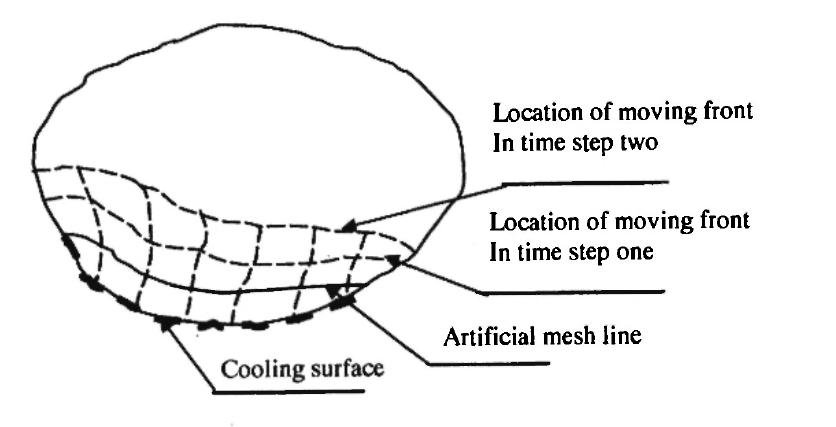
\includegraphics[width=5cm]{img/Newstefanproblemakjfjk.png}\\
  \caption{The mesh generation in Stefan problem 2D. (Figure taken from \cite{Wu+2005+281+288}}
  \label{fig:New mesh generation}
\end{figure}
\begin{figure}[htb]
  \centering
  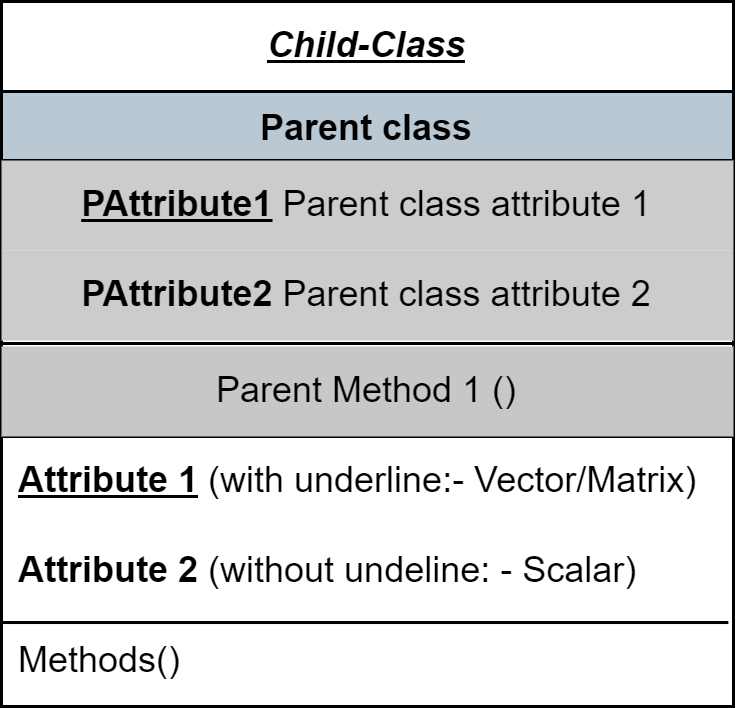
\includegraphics[width=5cm]{img/Nomenclature_Class.png}\\
  \caption{Structure of Class}
  \label{fig:Structure_of_class}
\end{figure}

\begin{figure}[htb]
  \centering
  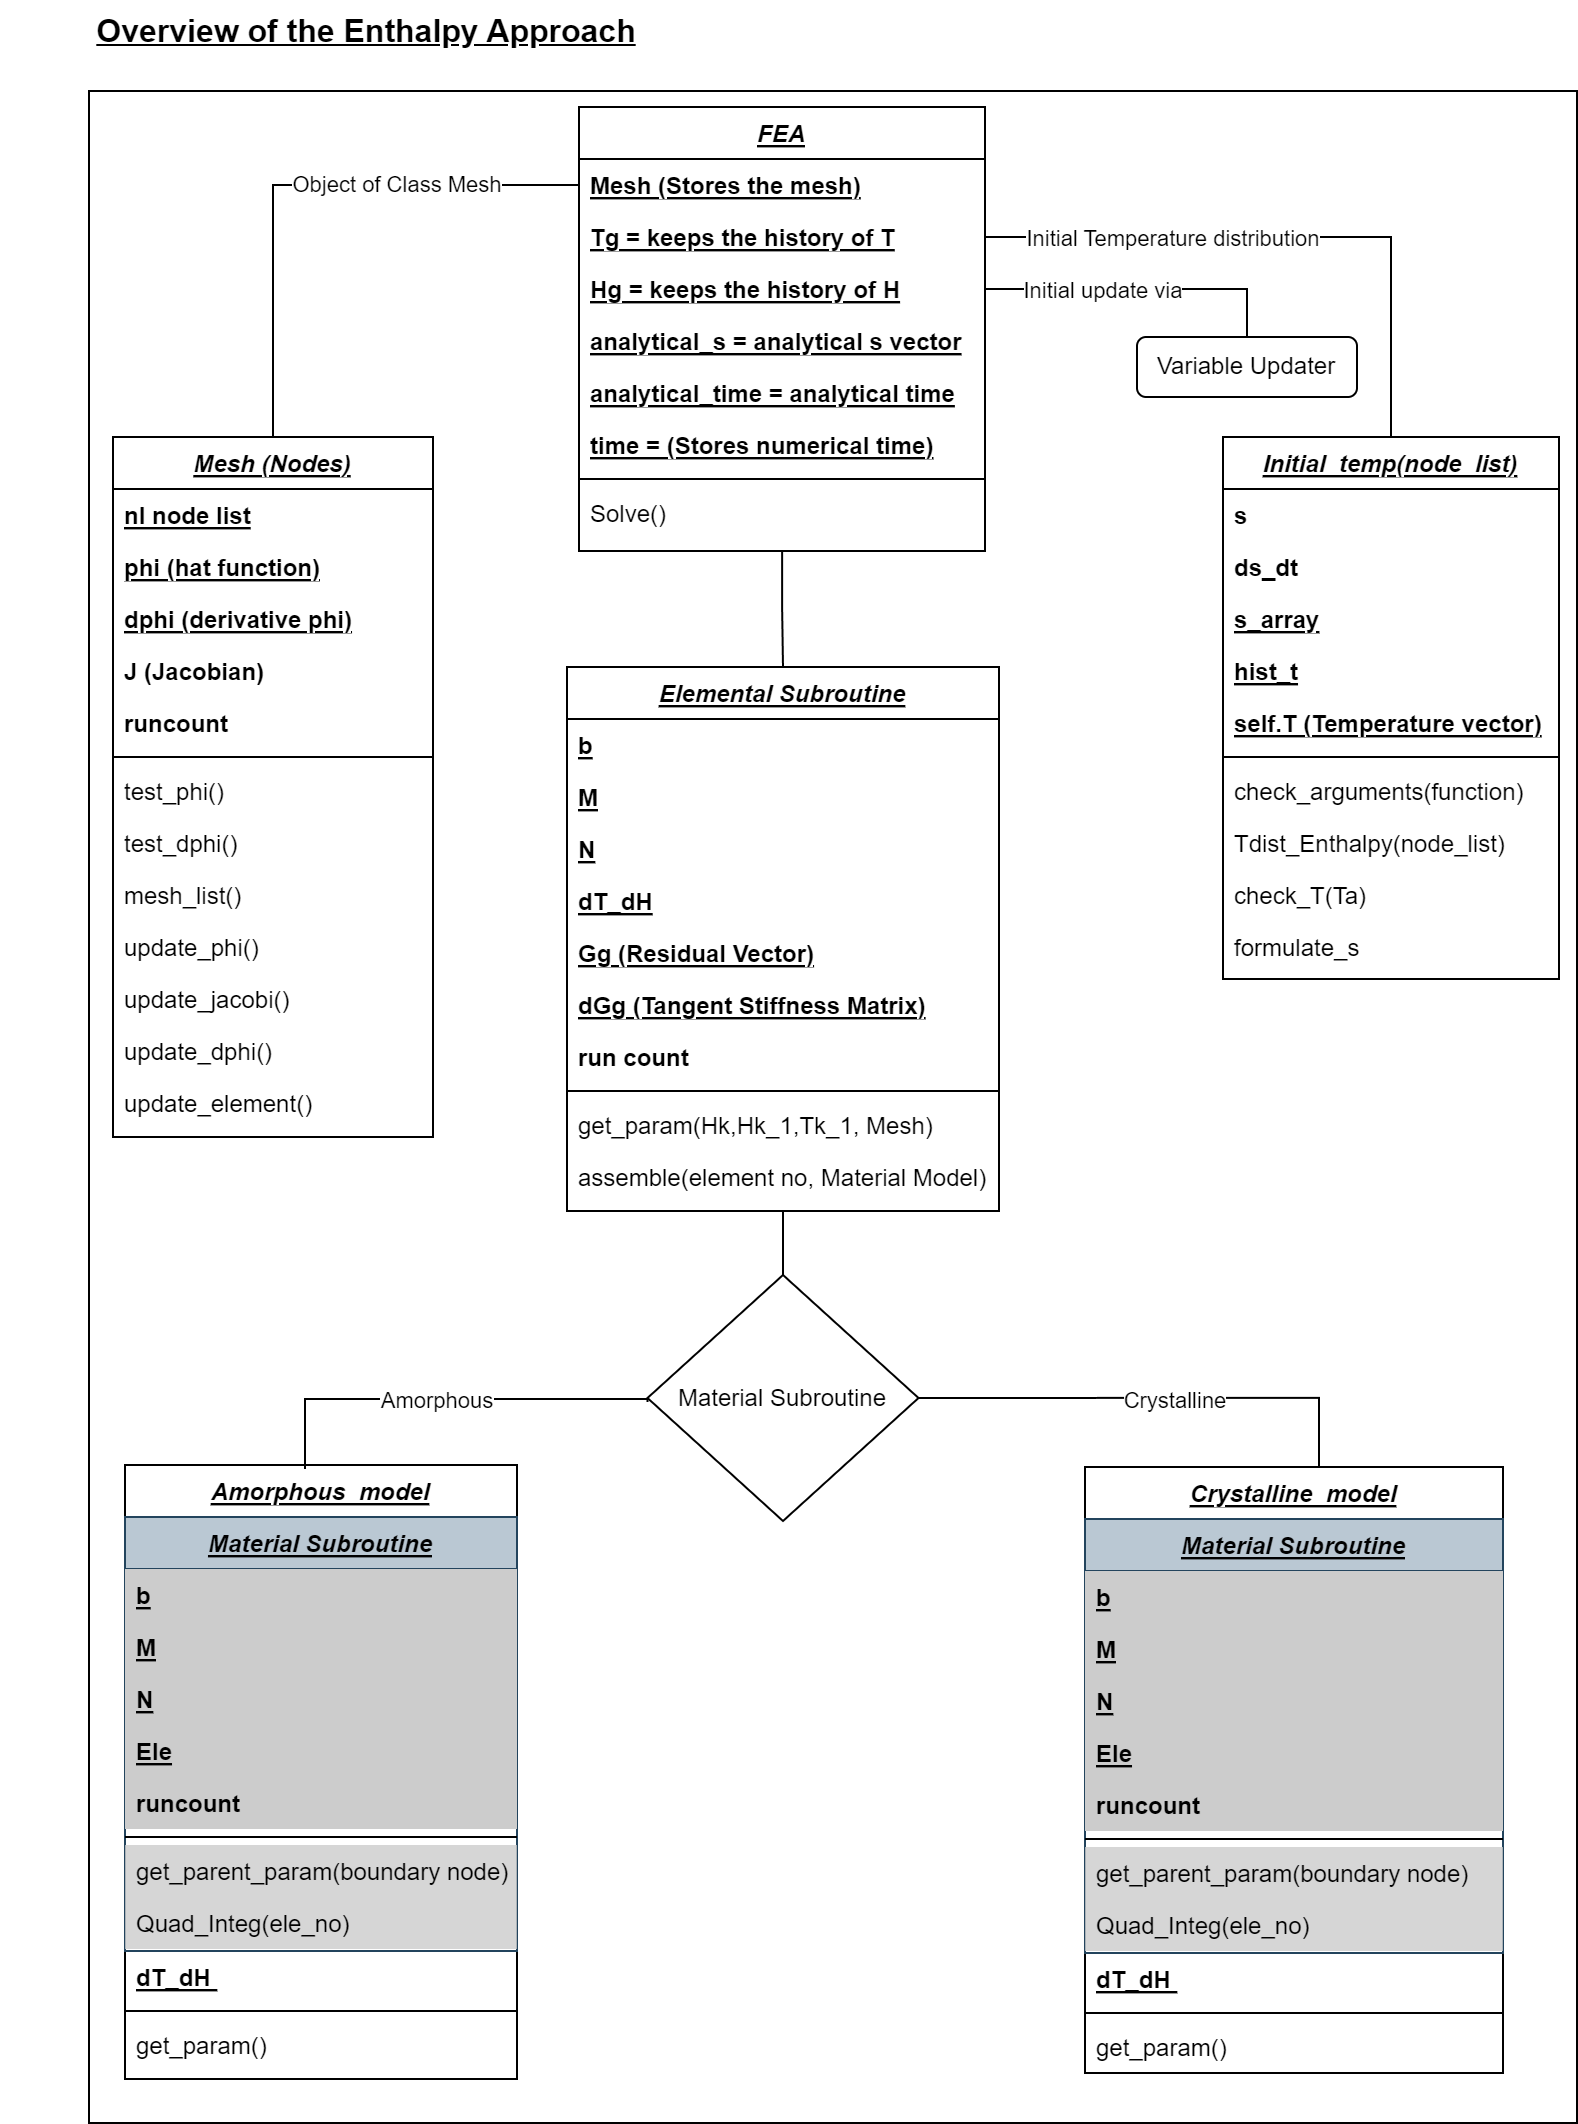
\includegraphics[width=14.3cm]{img/Over_View.png}\\
  \caption{Overview of the Enthalpy Problem Approach}
  \label{fig:Initial_temp}
\end{figure}

\begin{figure}[htb]
  \centering
  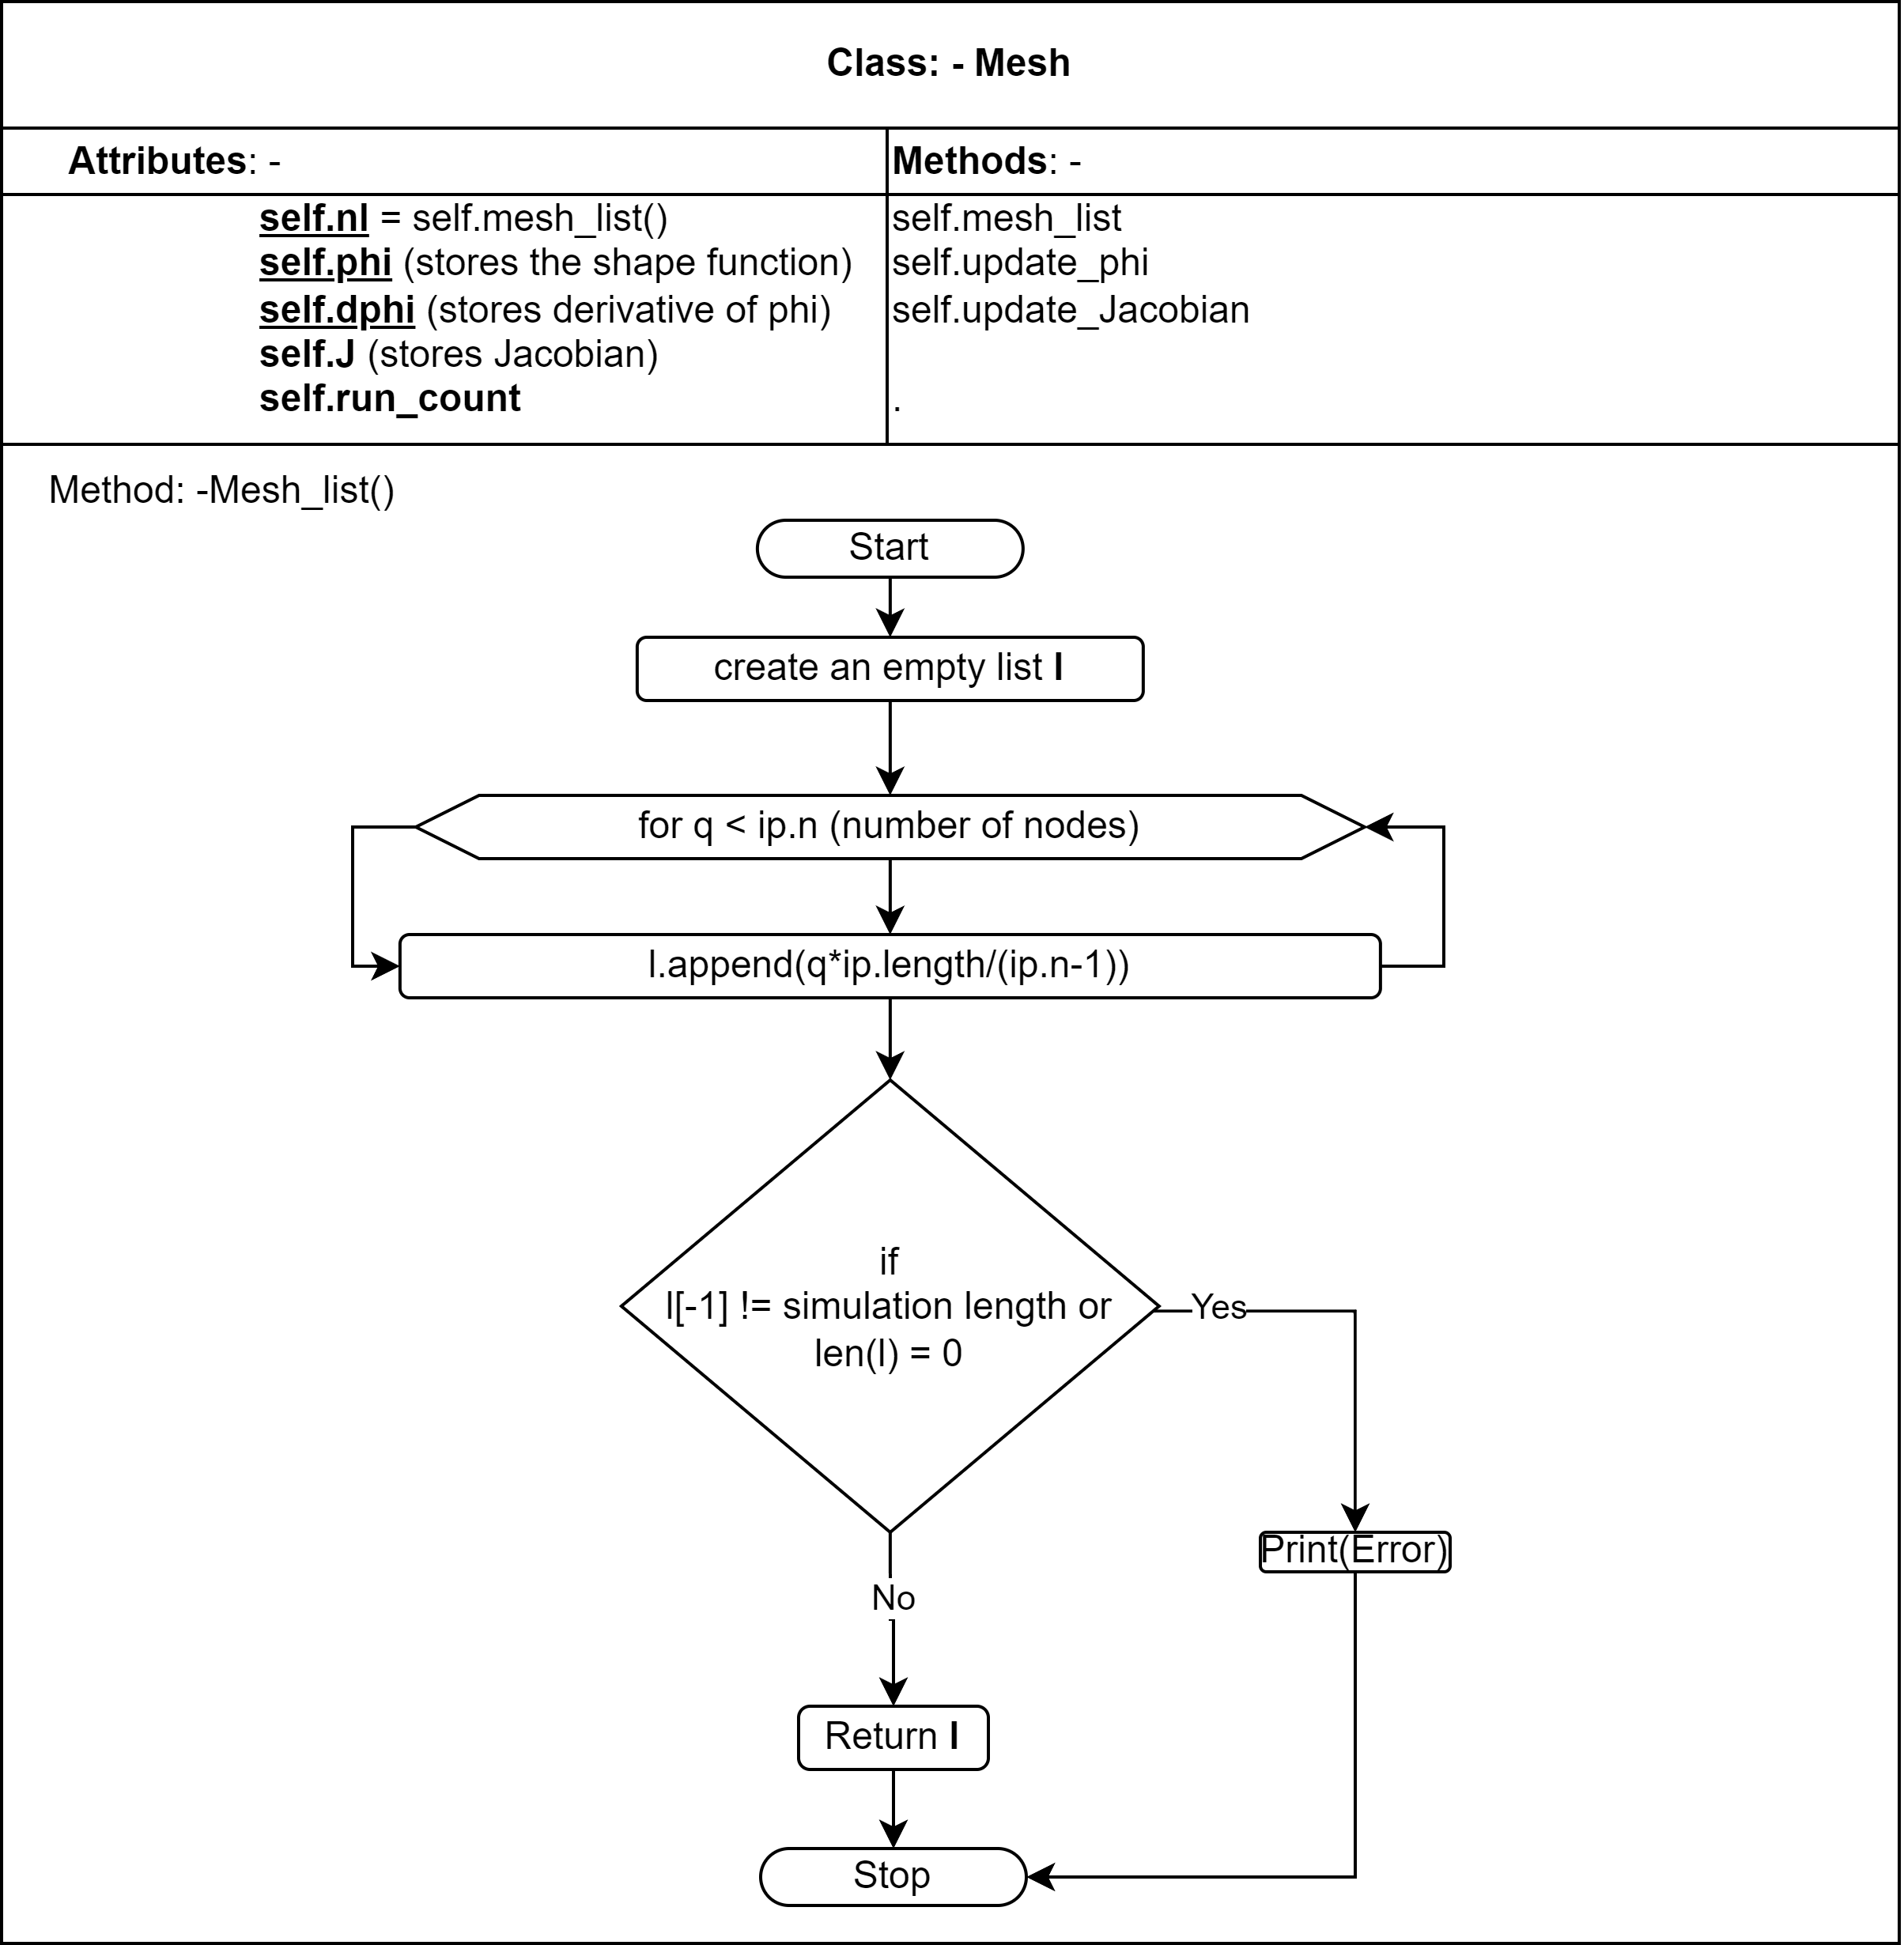
\includegraphics[width=13cm]{img/Mesh.png}\\
  \caption{Mesh}
  \label{fig:Mesh}
\end{figure}

\begin{figure}[htb]
  \centering
  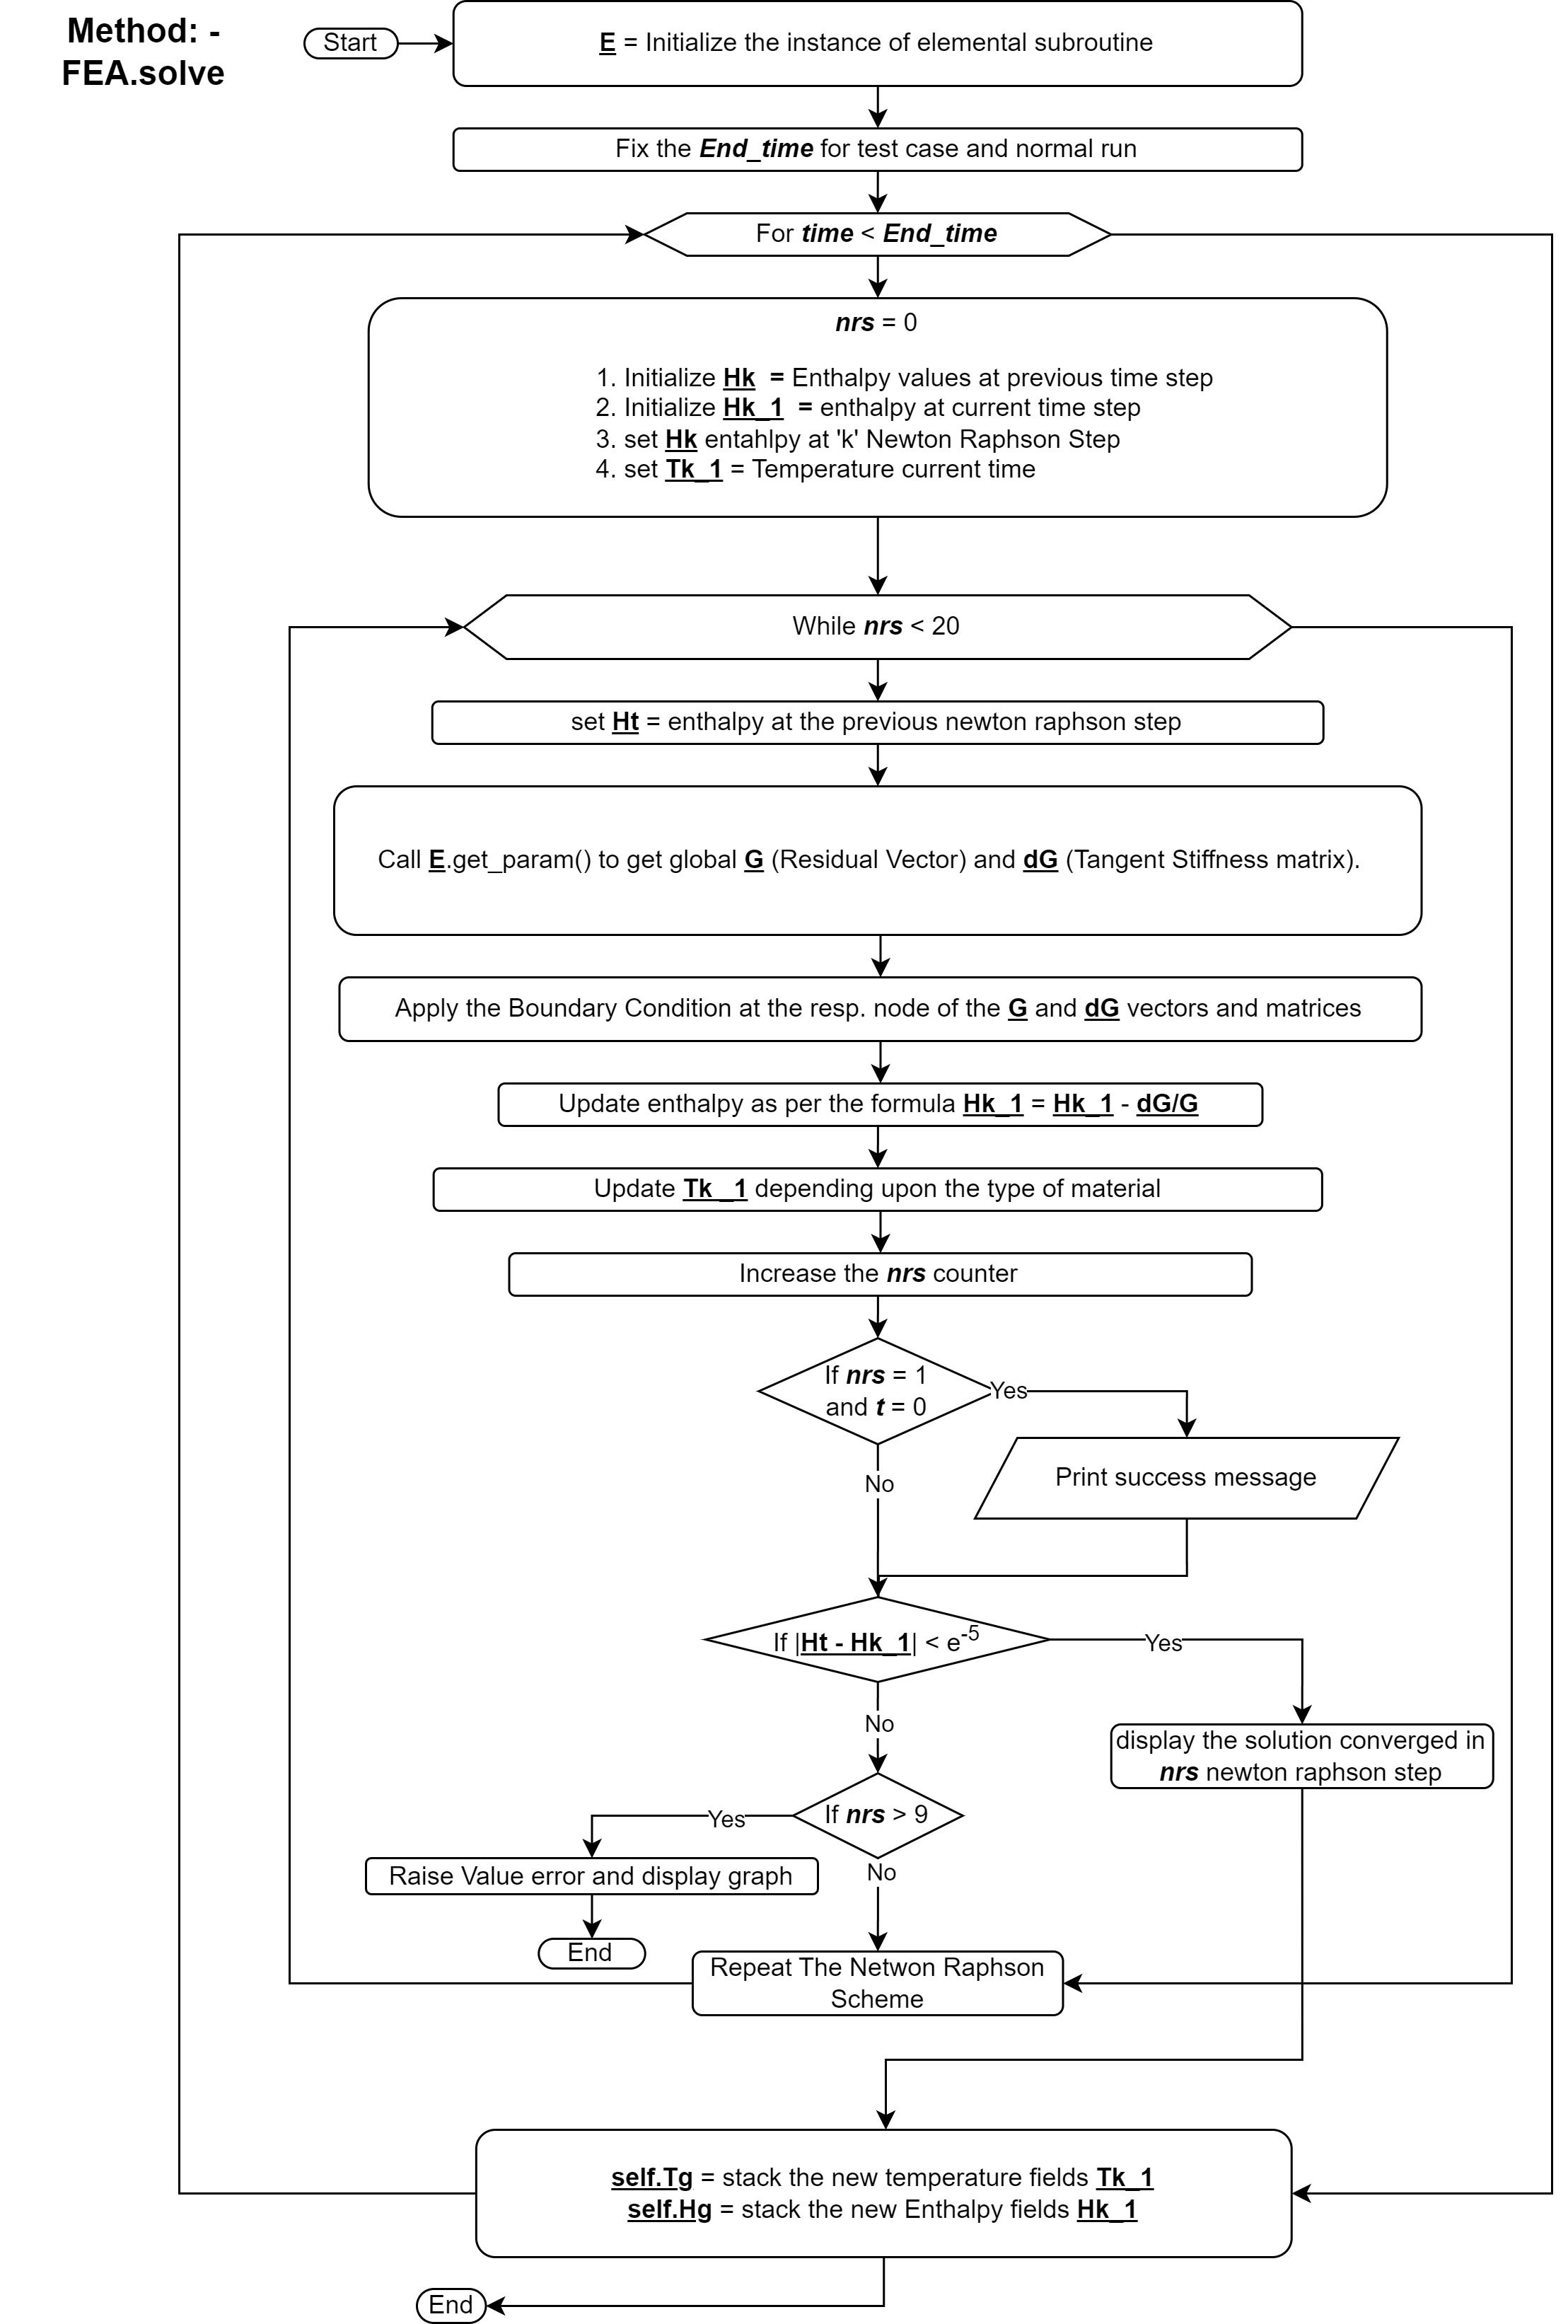
\includegraphics[width=13cm]{img/FEA_Solve.png}\\
  \caption{Main Class FEA}
  \label{fig:FEA_Solve}
\end{figure}

\begin{figure}[htb]
  \centering
  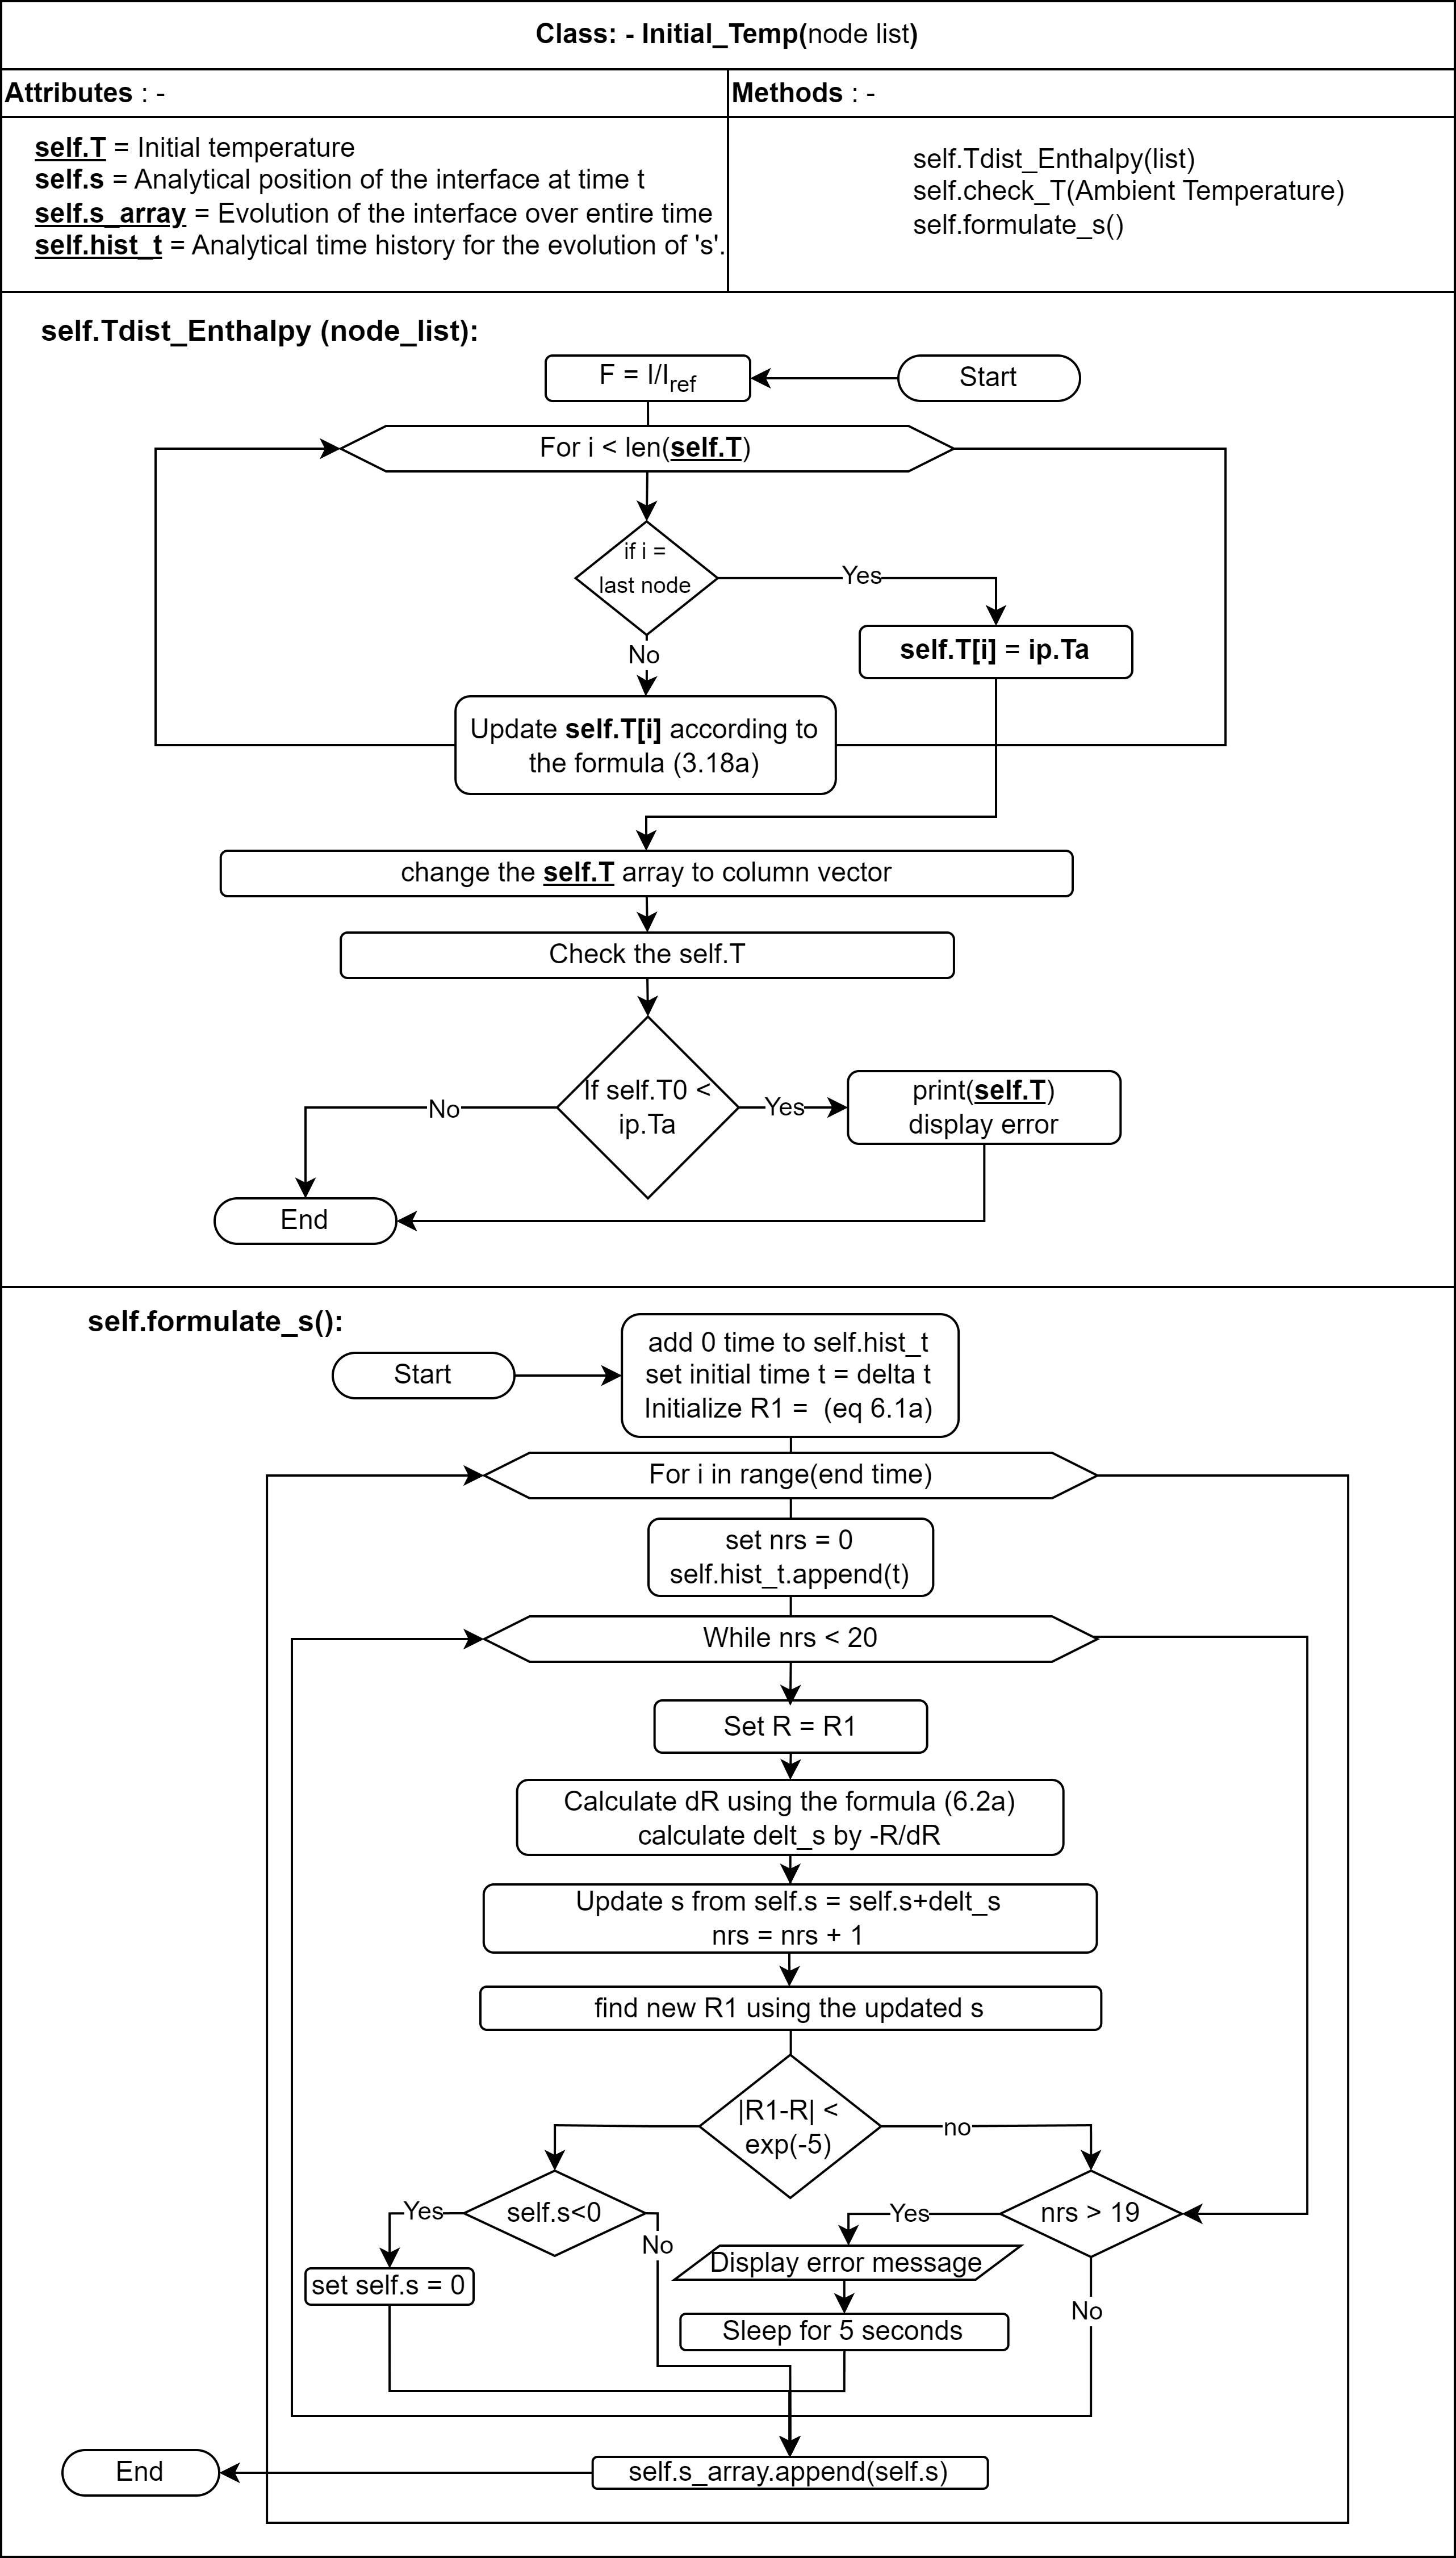
\includegraphics[width=11cm]{img/drawio.png}\\
  \caption{Class Initial Conditions}
  \label{fig:Initial Conditions}
\end{figure}

\begin{figure}[htb]
  \centering
  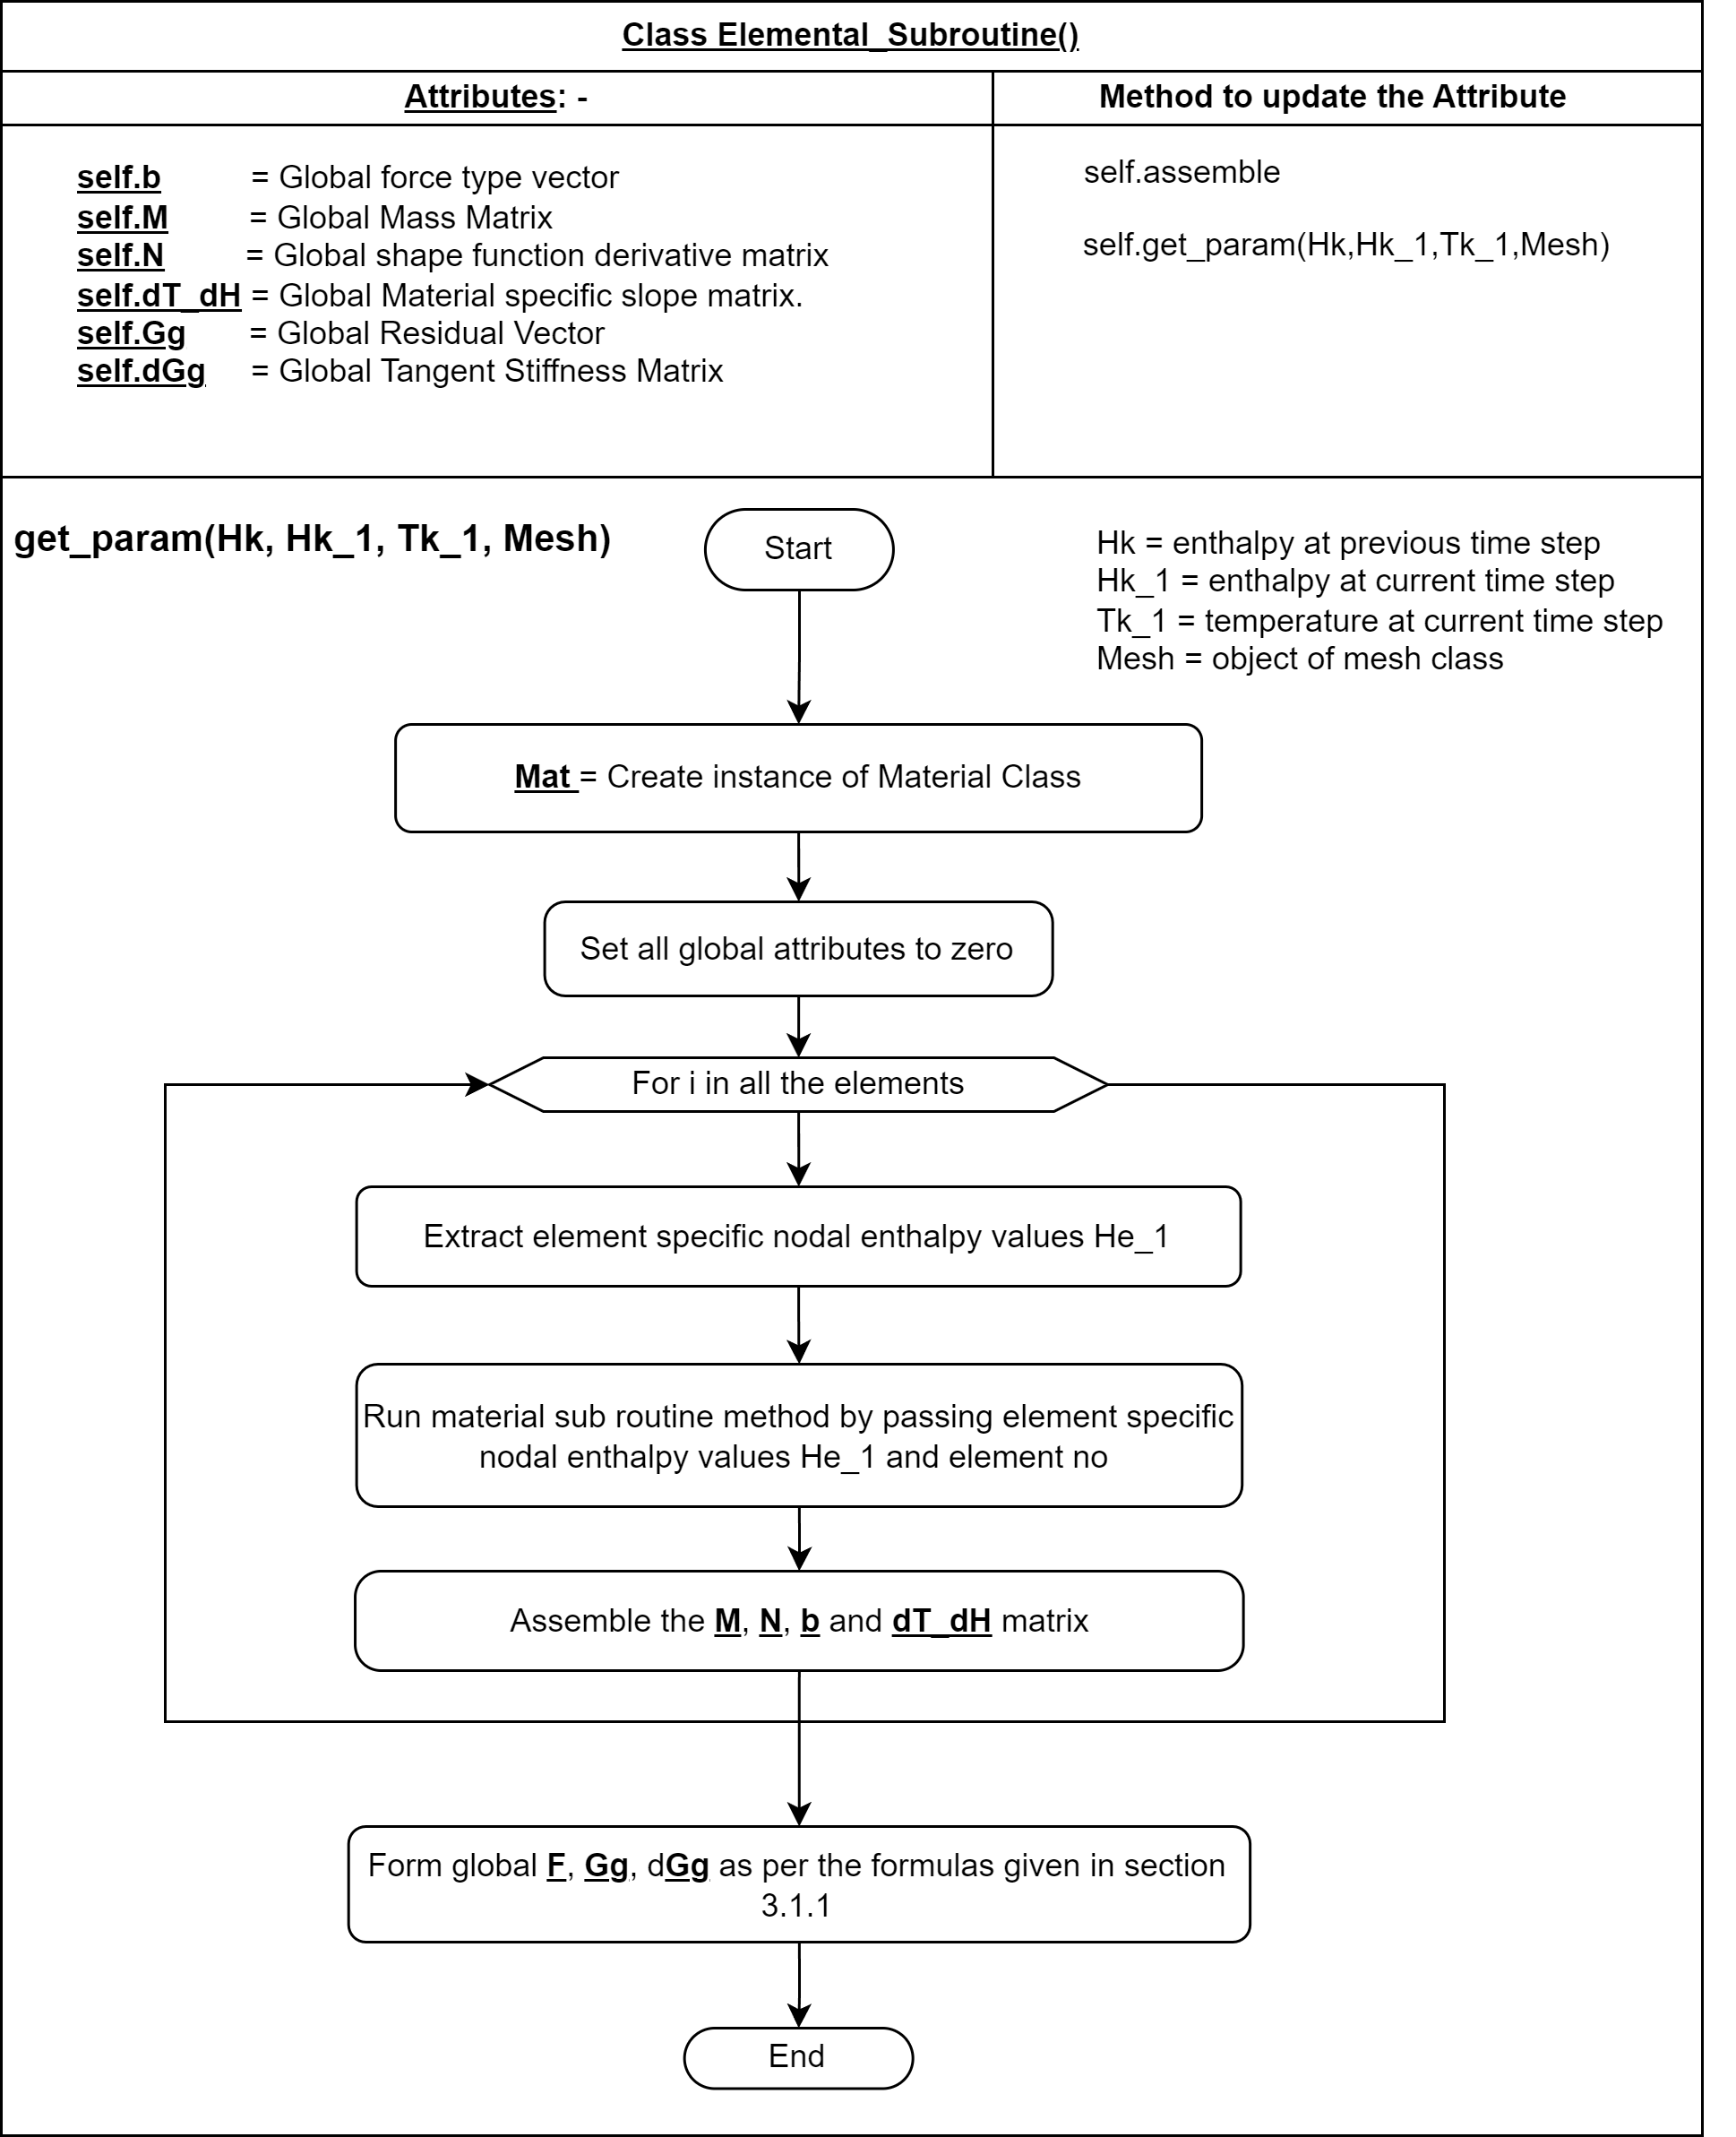
\includegraphics[width=13cm]{img/ElementalSubroution.drawio.png}\\
  \caption{Class Elemental Subroutine}
  \label{fig:Elemental Subroution}
\end{figure}
\begin{figure}[htb]
  \centering
  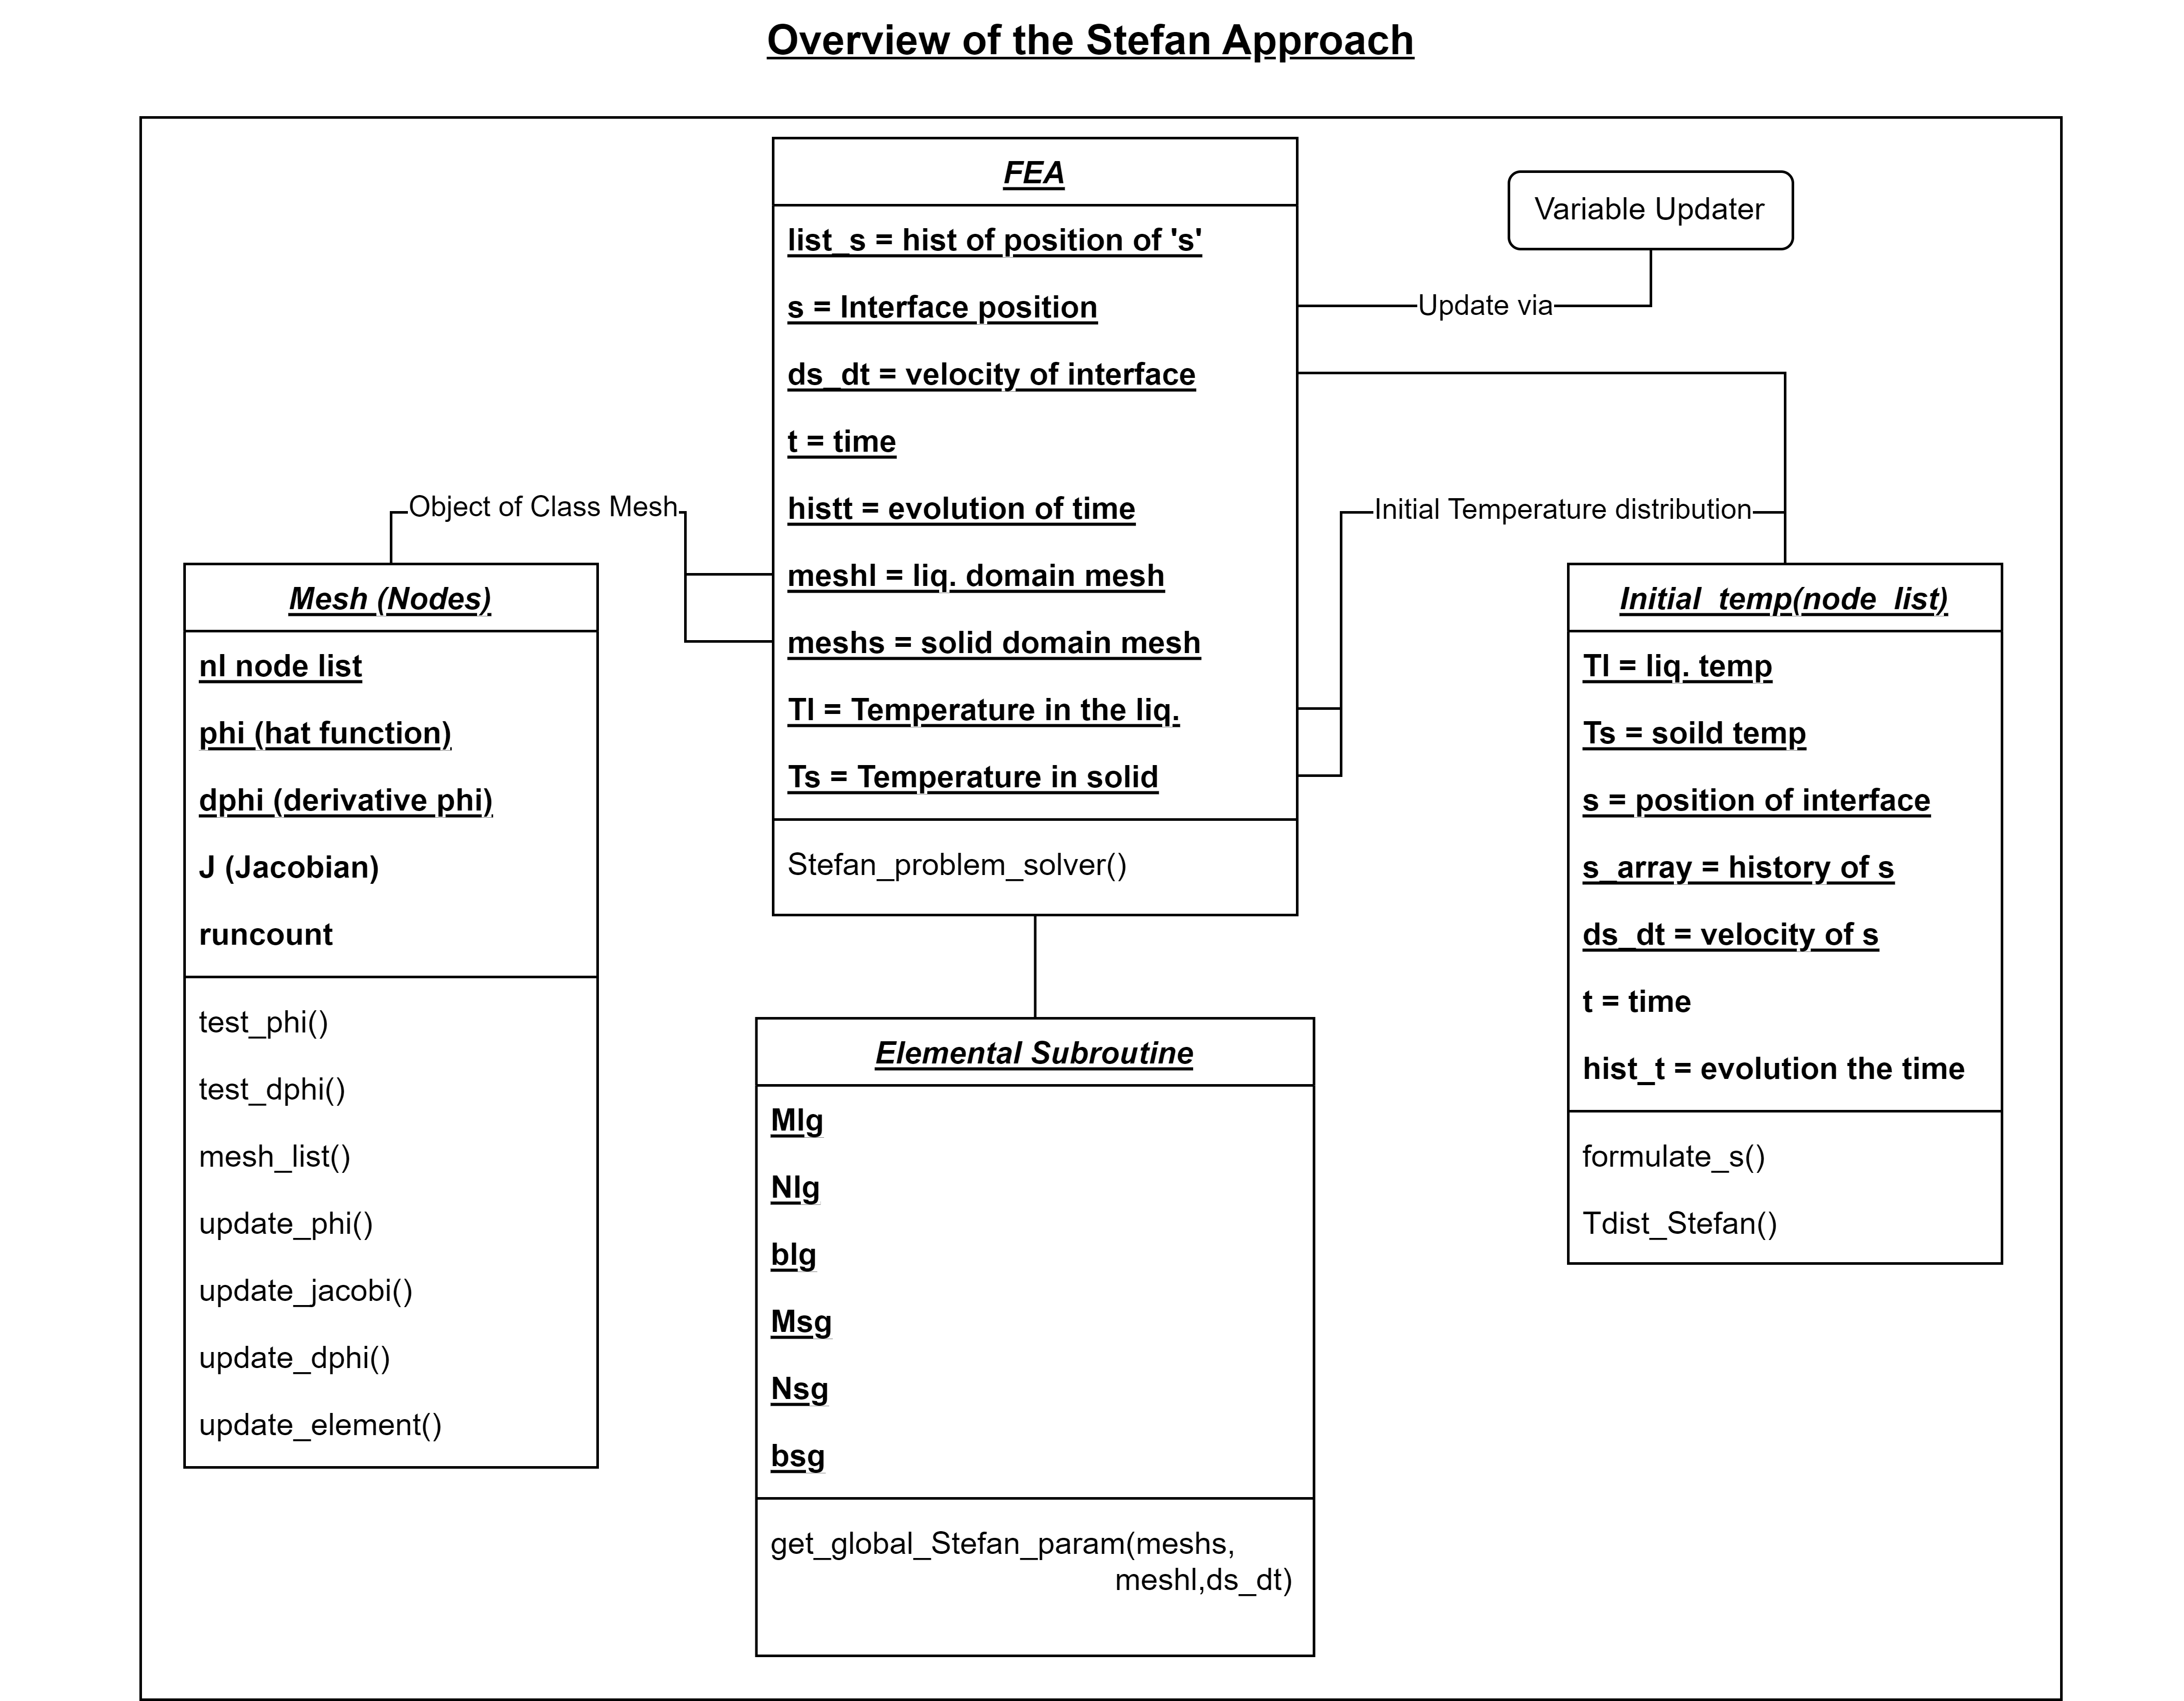
\includegraphics[width=13cm]{img/Stefan_Overview.png}\\
  \caption{Overview of the Stefan Problem Approach}
  \label{fig:overview Stefan Subroution}
\end{figure}
\begin{figure}[htb]
  \centering
  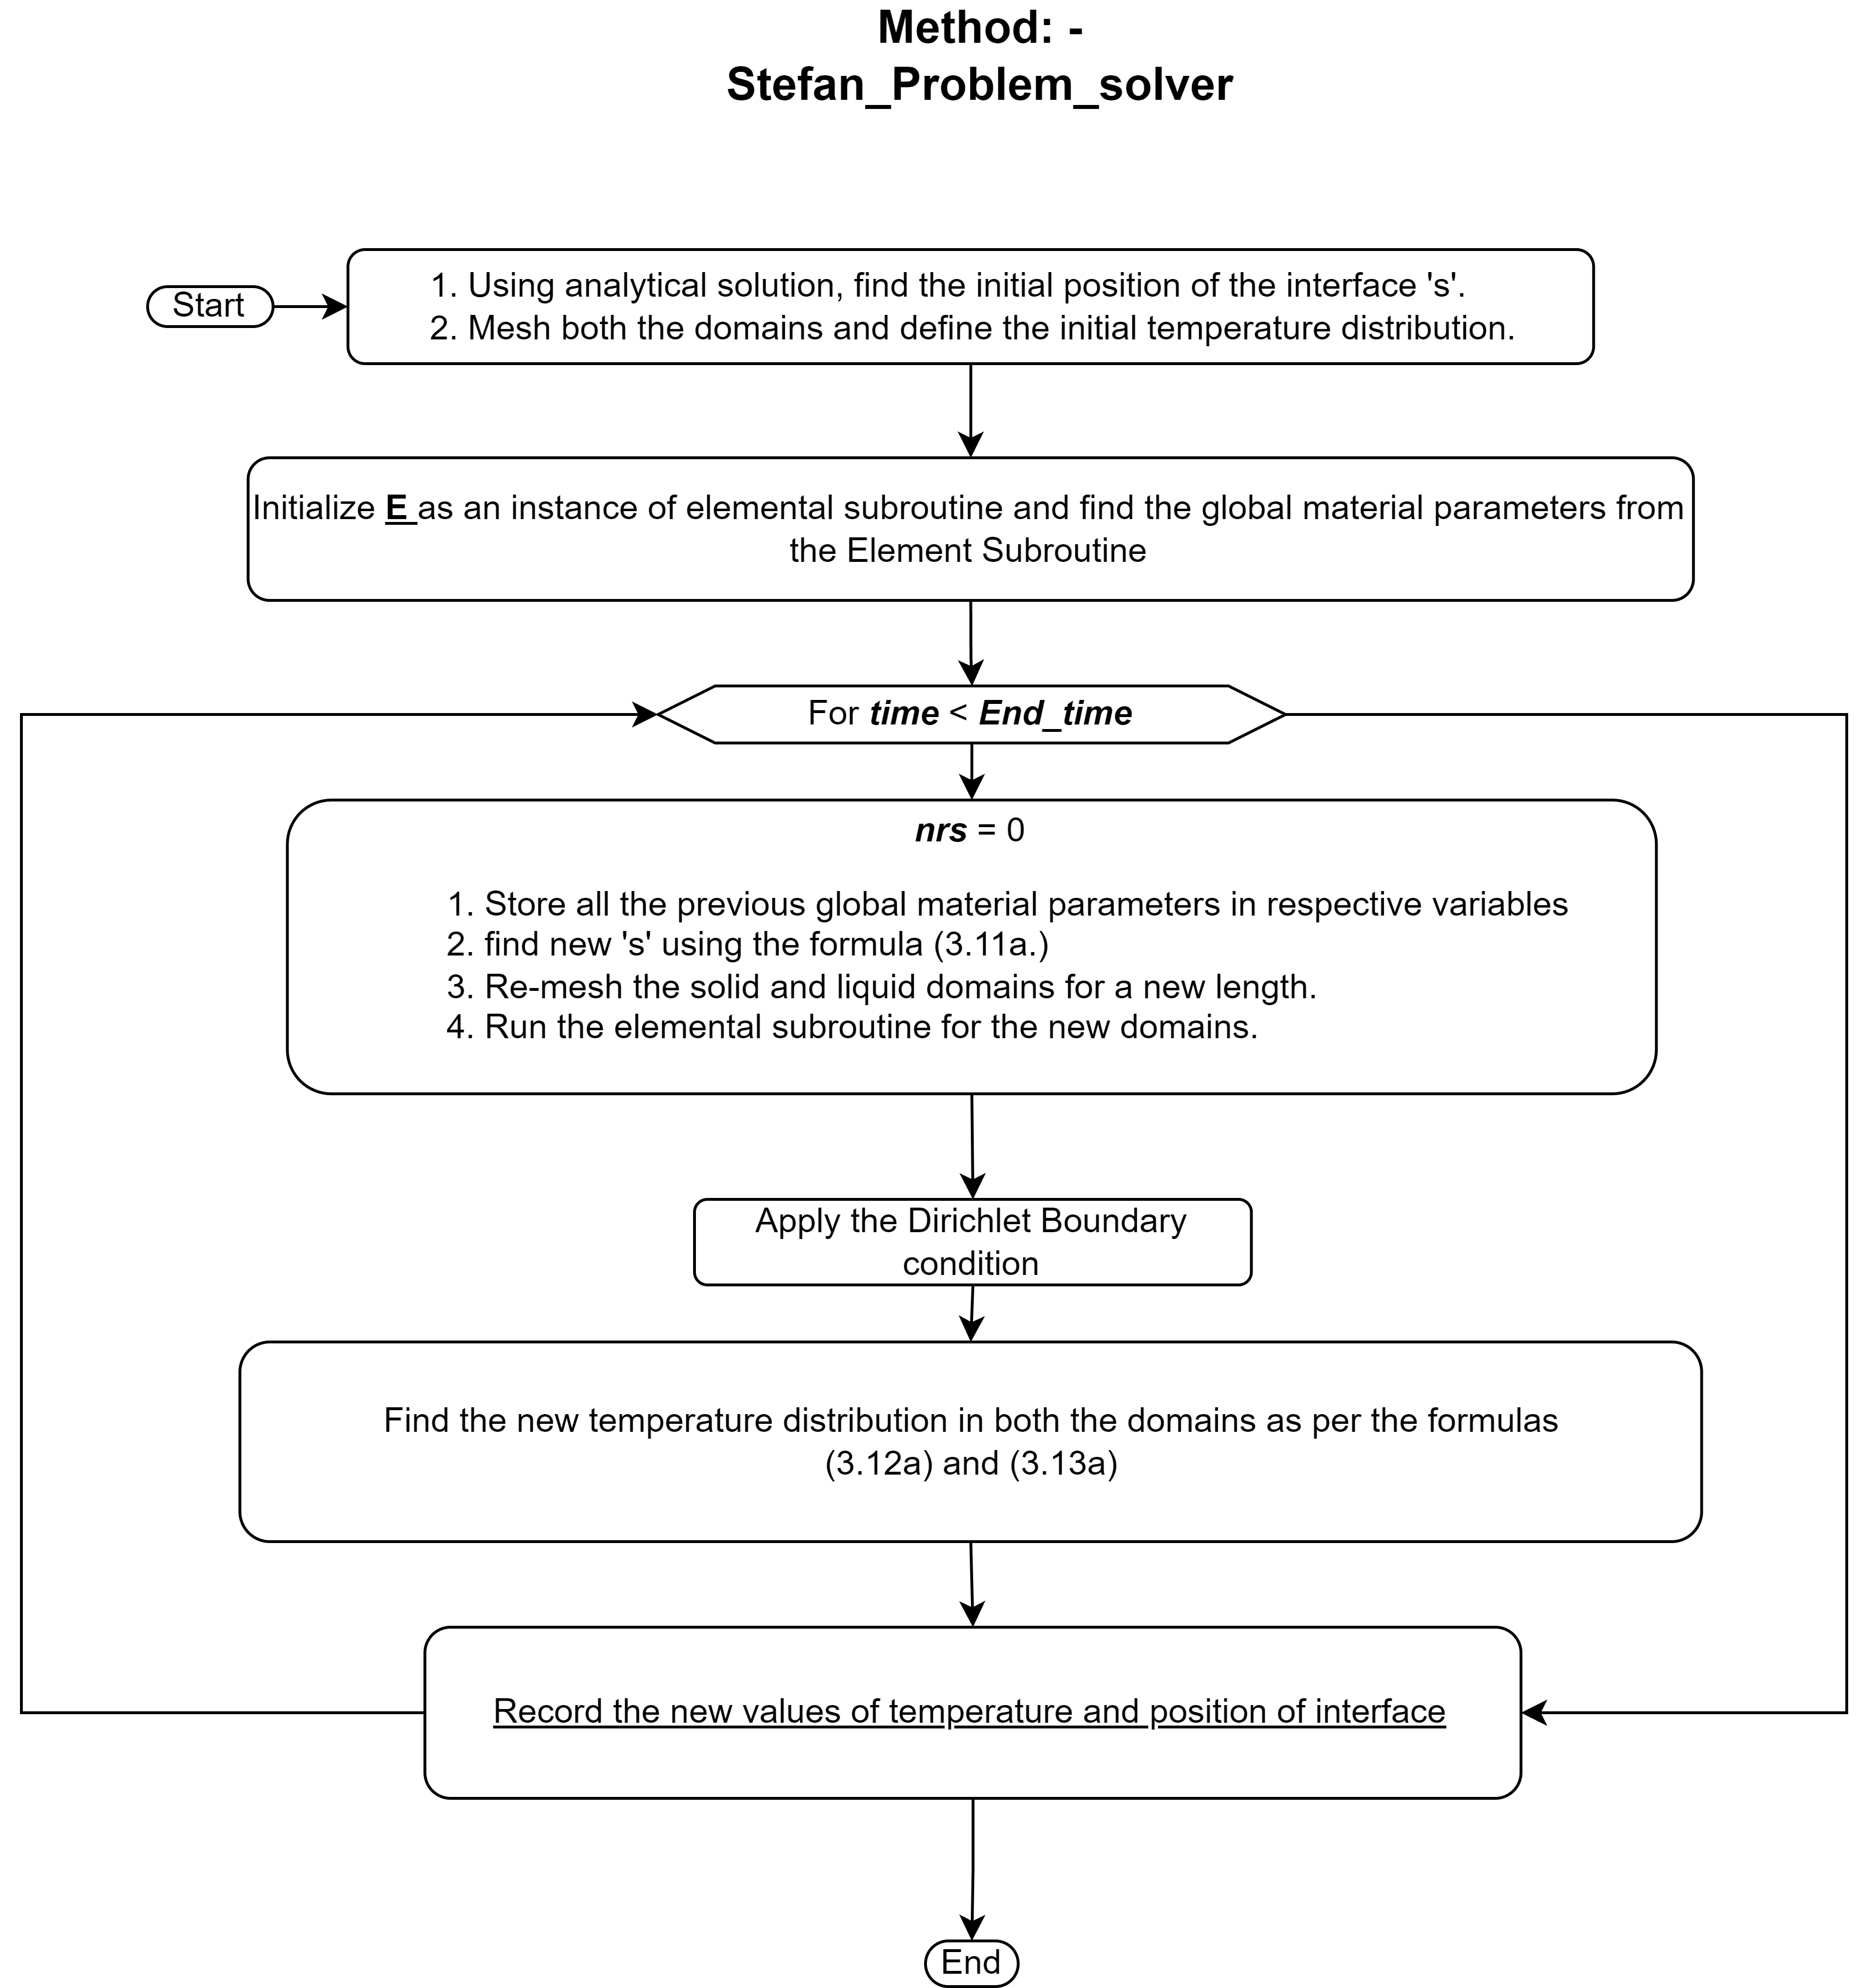
\includegraphics[width=13cm]{img/Stefan_Problem.png}\\
  \caption{Stefan Problem Solver}
  \label{fig:Stefan Problem Solver}
\end{figure}

    \chapter{Testing\label{cha:chapter4}}
\section{Unit Testing}
In this section we discuss the testing of the material specific libraries and the meshing library.\\
In the code, we have set the run count variable = 3, as for the very first run at time = 0 and run count = 0, the program outputs which type of material was detected as a check point to ensure proper functioning of the program. We refer to all the physical quantities as dimensionless quantities unless specified. For all testing purpose, we have assumed the length for the simulation to be 1 unit and the number of nodes to be 100.
\subsection{Test temperature enthalpy relation for amorphous material}
I will reiterate the temperature enthalpy relation for the amorphous material here for ease of reference within this section.\\ 
$\text{H(T)} =
\begin{cases}
D_2 T, & T \leq 0, \\ \\
D_2 T+ D_2 \lambda_f \frac{T}{T_{liq}}, & 0 \leq T \leq T_{liq}, \\ \\
D_2 T + D_2\lambda_f, & T > T_{liq}
\end{cases}\quad\text{for amorphous materials}$\\ \\
\underline{Aim:} To check whether $\frac{\partial T}{\partial H}(H)$ in the user defined material model in the equation \ref{eq:Decretized_dG_matrix} functions correctly.\\ \\
\underline{Risks:} It is an important part of the material model as it defines the relation of temperature with the enthalpy. If this part of the code fails especially at the phase change, inaccurate slope values will be generated leading to an inaccurate position of the interface or may produce nonphysical results. The most important part is when the nodal non dimensional enthalpy is close to 0 or $H_{liq}$ as these are the points of sharp transition and sudden changes in the slope. Hence, we mainly focus on these inputs.\\ \\
\underline{Values of interest:} The enthalpy value between 0 and $H_{liq}$ are of concern as the slope changes here and attains the value $\frac{T_{\text{liq}}}{D T_{\text{liq}} + D \lambda_{f}}$. In the liquid and the solid phase the slope is simply defined by $\frac{1}{D}$. \\

\noindent \underline{Inputs required:} For this function we need to provide the inputs in the following form dT\textunderscore dH [material type, nodal Enthalpy values, run count], material type = 1 shows it is a crystalline material and 2 indicates its an amorphous material. $H_{liq}$ is the dimensionless enthalpy at the liquidus temperature calculated as per the equation \ref{eq:liqudiousnonenahlpy},  Below we discuss the various nodal values of the $H_{liq}$ that were passed as an input.\\ \\
\underline{Input:} [-1, $H_{\text{liq}}$+0.5]\\ \\
\underline{Output Expected:}
\[
\begin{bmatrix}
\frac{1}{D} & 0 \\
0 & \frac{1}{D}
\end{bmatrix}
\]
\underline{Reason for the Output Expected:} Enthalpy = -1 indicates material is still in solid phase and the $H_{\text{liq}}$+0.5 indicate that material is in liquid state. For both the inputs the slope is defined as $\frac{1}{D}$\\ \\
\underline{Status:} Passed\\

\noindent \underline{Input:} [0, $H_{\text{liq}}$]\\ \\
\underline{Output Expected:}
\[
\begin{bmatrix}
\frac{1}{D} & 0 \\
0 & \frac{T_{\text{liq}}}{D T_{\text{liq}} + D \lambda_{f}}
\end{bmatrix}
\]
\underline{Reason for the Output Expected:} Enthalpy equal to 0 indicates that the material is starting to undergo a phase change, and the temperature does not change. However, for amorphous materials, the slope changes after the enthalpy surpasses 0. $H_{\text{liq}}$ signifies that the material is undergoing a phase change, and the slope is determined by $\frac{T_{\text{liq}}}{D T_{\text{liq}} + D \lambda_{f}}$.\\ \\
\underline{Status:} Passed\\

\noindent \underline{Input:} [0.000001, $H_{\text{liq}}$+0.000001]\\ \\
\underline{Output Expected:}
\[
\begin{bmatrix}
\frac{T_{\text{liq}}}{D T_{\text{liq}} + D \lambda_{f}} & 0 \\
0 & \frac{1}{D}
\end{bmatrix}
\]
\underline{Reason for the Output Expected:} The first nodal enthalpy shows that the material is changing phase and the second nodal enthalpy indicates that the material is in liquid state.\\ \\
\underline{Status:} Passed\\

\noindent \underline{Input:} [0, $H_{\text{liq}}$-0.000001]\\ \\

\noindent \underline{Output Expected:}
\[
\begin{bmatrix}
\frac{1}{D} & 0 \\
0 & \frac{T_{\text{liq}}}{D T_{\text{liq}} + D \lambda_{f}}
\end{bmatrix}
\]
\underline{Reason for the Output Expected:} The first nodal enthalpy shows that the material just started to change phase hence, considered to be in solid phase, and the second nodal enthalpy indicates that the material is in the phase change regime.\\ \\
\underline{Status:} Passed\\

\noindent \underline{Command for the test:} pytest Test\textunderscore Amorphous.py\\

\subsection{Test temperature enthalpy relation for crystalline material}
I will reiterate the temperature enthalpy relation for the crystalline material here for ease of reference within this section.\\
$\text{H(T)} =
\begin{cases}
D_1 T, & \text{T < 0}, \\ \\
[0, D_1 \lambda_f], & \text{T = 0}, \\ \\
D_1 T + D_1\lambda_f, & \text{T > 0}
\end{cases}\quad\quad\quad\quad\quad\text{for crystalline materials}$ \\ \\
\underline{Aim:} The objective is similar as discussed in the above section. The only difference is that the value of the slope changes. Here, the slope is zero during the phase change.\\ \\
\underline{Values of interest:} The enthalpy value between 0 and $D \lambda_f$ are of concern as the slope changes to 0 here. In the liquid and the solid phase the slope is simply defined by $\frac{1}{D}$. \\ \\
\underline{Input:} [-1, $D \lambda_\text{f}$]\\ \\
\noindent\underline{Output Expected:}
\[
\begin{bmatrix}
\frac{1}{D} & 0 \\
0 & 0
\end{bmatrix}
\]
\underline{Reason for the Output Expected:} Enthalpy = -1 indicates material is in solid state. $D \lambda_f$ shows that the material is in the phase change and the slope is 0.\\ \\
\underline{Status:} Passed\\

\noindent \underline{Input:} [0, $D \lambda_\text{f} + 0.5$]\\ \\
\underline{Output Expected:}
\[
\begin{bmatrix}
0 & 0 \\
0 & \frac{1}{D}
\end{bmatrix}
\]
\underline{Reason for the Output Expected:} Enthalpy = 0 indicates material in phase change process and the slope is 0. $D \lambda_f$ +0.5 shows that the material is in the liquid phase.\\ \\
\underline{Status:} Passed\\

\noindent\underline{Input:} [$\lambda_\text{f} , -1$]\\ \\
\noindent\underline{Output Expected:}
\[
\begin{bmatrix}
\frac{1}{D} & 0 \\
0 & \frac{1}{D}
\end{bmatrix}
\]
\underline{Reason for the Output Expected:} Both the nodal enthalpies indicate material in liquid and solid state respectively.\\ \\
\underline{Status:} Passed\\

\noindent \underline{Input:} [0, $D \lambda_f$] \\ \\

\noindent \underline{Output Expected:}
\[
\begin{bmatrix}
0 & 0 \\
0 & 0
\end{bmatrix}
\]
\underline{Reason for the Output Expected:} Both the nodal enthalpies indicate material under going phase change.\\ \\
\underline{Status:} Passed\\

\noindent \underline{Command for the test:} pytest Test\textunderscore Crystalline.py\\

\subsection{Test Shape Function Derivative}
\underline{Aim:} The derivative of the shape function describe the change of the open coefficients (in our case temperature) with respect to space. This is completely different than the slopes described above. In the above section, we tested the change of temperature with respect to enthalpy and not with respect to space. The objective is to check if the shape function were correctly derived. \\ \\

\noindent \underline{Input:} [2, 1]\\ \\
\underline{Expected Output:} -100.\\ \\
\underline{Reason for the Output Expected:}  Since, the length of the material is 1 unit and the number of nodes are 100, we know that the elemental length $l_e$ will be 0.01. By the definition of the derivative $\frac{T_2-T_1}{l_e}$ we have $\frac{1-2}{0.01}$ = -100.\\ \\
\underline{Status:} Passed\\ \\

\noindent \underline{Input:} [1, 3]\\ \\
\underline{Expected Output:} 200.\\ \\
\underline{Reason for the Output Expected:} Since, the length of the material is 1 unit and the number of nodes are 100, we know that 0.01 will be the elemental length $l_e$. By the definition of the derivative $\frac{T_2-T_1}{l_e}$ we have $\frac{3-1}{0.01}$ = 200.\\ \\
\underline{Status:} Passed\\ \\
\noindent \underline{Input:} [4, 4]\\ \\
\underline{Expected Output:} 0.\\ \\
\underline{Reason for the Output Expected:}  Since, the length of the material is 1 unit and the number of nodes are 100, we know that the elemental length $l_e$ will be 0.01.. By the definition of the derivative $\frac{T_2-T_1}{l_e}$ we have $\frac{4-4}{0.01}$ = 0.\\ \\
\underline{Status:} Passed\\ 
\noindent \underline{Command for the test:} pytest Mesh\textunderscore Test.py\\

\subsection{Test Partition of Unity}
\underline{Aim:} The shape functions are used to interpolate the values of the open coefficients at the nodes within the element. The partition of unit test is used to check if the sum of the shape functions at any point within the element is equal to 1. Failing this check means that the physical quantity of interest is not conserved within the element leading to incorrect calculation or definition of the shape function.\\ \\
\noindent \underline{Input:}[0.5] (value of local co-ordinate).\\ \\
\underline{Expected Output:} 1\\ \\
\underline{Reason for the Output Expected:} Property of the shape function.\\ \\
\underline{Status:} Passed\\ \\
\noindent \underline{Command for the test:} pytest Mesh\textunderscore Test.py\\

\subsection{Test Jacobian}
\underline{Aim:} To check if the determinant of Jacobian is positive. Since we work with linear shape functions, our Jacobian will be exactly half of the elemental length. Failing this test means that the geometry is not being conserved correctly.\\ \\
\noindent \underline{Input:} [2] (element number).\\ \\
\underline{Expected Output:} $\frac{(x_3-x_2)}{2} $ \\ \\
\underline{Reason for the Expected Output:} Here $x_3$ = global $x$ co-ordinate of the third node and $x_2$ = global $x$ co-ordinate of the second node\\ \\
\underline{Status:} Passed\\ \\
\noindent \underline{Command for the test:} pytest Mesh\textunderscore Test.py\\

\section{Unit Tests 2D}
We have created an instance of 2D mesh class by creating 5 x 5 nodes and assuming the length of the square to be 1 unit. All the tests were performed for element 3. 
\subsection{Test Partition of Unity}
\underline{Aim:} This is similar to the 1D partition of unity test. However, here we pass the Gauss quadrature points and iterate over all the points, and  for every iteration we check if the sum of the shape function is equal to 1. The weights for these points are unity.\\ \\
\noindent \underline{Input:} Gauss points = [-0.577350269189626, 0.577350269189626].\\ \\
\underline{Expected Output:} 1\\ \\
\underline{Status:} Passed\\ \\
\noindent \underline{Command for the test:} pytest Test\textunderscore Mesh\textunderscore 2D.py\\

\subsection{Test Jacobian}
\underline{Aim:} To check the determinant of the Jacobian is always positive and the sum of the determinant of the Jacobian over the Gauss quadrature is equal to the area of the element.\\ \\
\noindent \underline{Input:} Gauss points = [-0.577350269189626, 0.577350269189626].\\ \\
\underline{Expected Output:} $(x_2-x_0) \times (y_2-y_0)$ \\ \\
\underline{Reason for the Expected Output:} The determinant of the Jacobian is equal to the area of the element. It is the scaling factor by which the area changes during the transformation of the global co-ordinates to isoparametric co-ordinates. Also, in our mesh for an element, $x_2 = x_1$, $x_0 = x_3$, $y_2 = y_1$ and $y_0 = y_3$.\\ \\
\underline{Status:} Passed\\ \\
\noindent \underline{Command for the test:} pytest Test\textunderscore Mesh\textunderscore 2D.py\\

\subsection{Test derivative of the shape function}
\underline{Aim:} It is the same test as the 'Test Shape Function Derivative' in 1D, here we check it for 2D.\\ \\
\noindent \underline{Input:} We check the derivative on the nodal points hence we pass $\xi$ = 1 and $\eta$ = 1 (local co-ordinates) for the third element. The nodal temperature was [1,2,3,4]. \\ \\
\underline{Expected Output:} 1) $\frac{T_2-T_3}{(x_2-x_0)}$\\
\indent \indent \indent \indent \indent \indent \indent \indent \ 2) $\frac{T_2-T_1}{(y_2-y_0)}$\\ \\
\underline{Reason for the Expected Output:} Due to the input local co-ordinates, the derivative of shape function wrt $x$ has entries in 2 and 3 and for $y$ we have entries in 1 and 2 all other entries in the $dN$ vector are 0.\\ \\
\underline{Status:} Passed\\ \\

\noindent \underline{Command for the test:} pytest Test\textunderscore Mesh\textunderscore 2D.py\\
    \chapter{Verification\label{cha:chapter5}}
This chapter discusses the verification carried out to ensure proper working of our code. The results for the same will be discussed in Results and Discussion \ref{cha:chapter5}.

\section{Heat Transfer Verification in One Dimensional Settings for the Enthalpy Problem}
To verify the temperature distribution obtained from the numerical scheme, we compare the results obtained from the numerical scheme to the analytical one. We assume a one dimensional bar of unit length. We have considered two different types of boundary conditions, in order to verify the temperature distribution.\\

\noindent \textbf{A) Specified Temperature Boundary Condition (Type I BC): -}\\
 A boundary condition where both the ends of the bar are held at a constant fixed temperature is commonly referred to as specified temperature boundary condition\cite{Cengel_Ghajar_2020}. We assume, both the ends of the rod are at fixed 0 dimensionless temperature and $T_{initial} = f(x)$ as the initial temperature distribution, this means that our material is in liquid phase and there is no phase change. Mathematically we can write: -
 \begin{subequations}
     \begin{align}
         T(x,0) = T_{initial} = -\frac{1}{2}sin(3\pi x)+\frac{3}{2}sin(\pi x) \label{eq:type1initialBCS} \\ \nonumber
         \\
         T(0,t) \ = \ 0 \quad \text{and} \quad T(1,0) \ = \ 0 \label{eq:type1BCS}
     \end{align}
 \end{subequations}
 Figure \ref{fig:Type1_BC} depicts our setup for the heat transfer verification.\\
 The analytical solution for equation \eqref{eq:nondimensional} subject to initial \eqref{eq:type1initialBCS} and boundary \eqref{eq:type1BCS} conditions is given by equation \eqref{eq:AnalyticalBCS}\cite{Hancock}.
 \begin{subequations}
     \begin{align}
         T_{(x,t)} = \frac{3}{2}sin(\pi x)e^{-\pi^2 t}-\frac{1}{2}sin(3\pi x)e^{-9\pi^2 t} \label{eq:AnalyticalBCS}
     \end{align}
 \end{subequations}
 \begin{figure}[htb]
  \centering
  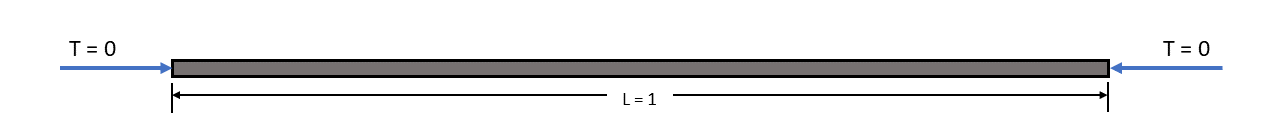
\includegraphics[width=11cm]{Type1_BC.png}\\
  \caption{Setup for the Heat Transfer Verification with type 1 boundary condition}
  \label{fig:Type1_BC}
\end{figure}\\
\noindent \textbf{B) Specified Heat Flux Boundary Condition (Type II BC): -}\\
A boundary condition where heat flux is specified at one end and the other end is assumed to be fixed at a dimensionless temperature is known as specified heat flux boundary condition\cite{Cengel_Ghajar_2020}. In our case, we  assume that the end x = 0 is insulated $\left(\frac{\partial T}{\partial x} =  0 \right)$, where as the other end x = 1 is at a fixed 0 dimensionless temperature ($T_{1,t} = $ 0) with $T_{initial} = T_{x,0}$ = 1 as the initial temperature distribution. The figure \ref{fig:Temperature_Distribution} shows the setup.  
\begin{figure}[htb]
  \centering
  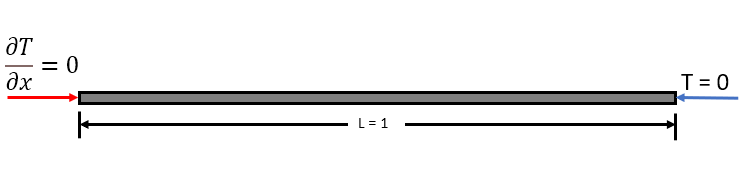
\includegraphics[width=9cm]{Testing.png}\\
  \caption{Setup for the Temperature Distribution Verification}
  \label{fig:Temperature_Distribution}
\end{figure}
The equation \eqref{eq:Analytical_Solution} \cite{Hancock}is the analytical solution to the temperature distribution over time for the equation \eqref{eq:nondimensional} subject to type 2 boundary condition.\\
\begin{subequations}
\begin{align}
    T(x,t) = \frac{4 T_{initial}}{\pi} \sum_{n=1}^{\infty} \frac{(-1)^{n+1}}{2n-1}cos \left ( \frac{2n-1}{2} \pi x \right) exp  \left (- \frac{(2n-1)^2 \pi^2}{4}t\right)\label{eq:Analytical_Solution}
\end{align}
\end{subequations}\\
where: -\\
\indent $T_{initial}$ = Constant Initial Temperature Distribution\\
\indent $t$ = Time\\
We have carried out the verification of the position of the interface for the one dimensional Stefan problem approach in the next chapter. 
    \chapter{Results and Discussion\label{cha:chapter6}}

This chapter describes the results obtained from the above two schemes. The quantities used below in this section are dimensionless unless specified. 
We have considered pure Aluminum as a crystalline material with sharp melting point and SS304L as an amorphous material which melts over a range of temperature. The properties of Al are summarized in the table \ref{table:AL}\cite{verhoeven2003modelling} and the properties of SS304 are summarized in the table \ref{table:SS304L}\cite{Zhou_2006}. 
\begin{table}[htbp]
    \centering
    \renewcommand{\arraystretch}{1.5} % Increase the row height by 1.5 times
    \begin{tabular}{|c|c|}
        \hline
         Property & Value \\
         \hline
         Thermal conductivity $k$ & $2.3 \ \text{x}\ 10^2\, \frac{W}{mK}$\\
         \hline
         Density $\rho$ & $2.7\ \text{x} \ 10^3\, \frac{kg}{m^3}$\\
         \hline
         Melting temperature $T_m$ & $9.3\ \text{x} \ 10^2 K$\\
         \hline
         Vapour temperature $T_v$ & $2.5 \ \text{x} \ 10^3 K$\\
         \hline
         Specific heat of the solid c & $9.0 \ \text{x} \ 10^2 \frac{J}{kg K}$\\
         \hline
         Latent heat of fusion $L_f$ & $3.6 \ \text{x} \ 10^5 \frac{J}{kg}$\\
         \hline
    \end{tabular}
    \caption{Properties of Al}
    \label{table:AL}
\end{table}\\

\begin{table}[htbp]
    \centering
    \renewcommand{\arraystretch}{1.5} % Increase the row height by 1.5 times
    \begin{tabular}{|c|c|}
        \hline
         Property & Value \\
         \hline
         Thermal conductivity $k$ & $22\, \frac{W}{mK}$\\
         \hline
         Density $\rho$ & $7.2\ \text{x} \ 10^3\, \frac{kg}{m^3}$\\
         \hline
         Solidus temperature $T_{sol}$ & $16.7\ \text{x} \ 10^2 K$\\
         \hline
         Liquidus temperature $T_{sol}$ & $17.27\ \text{x} \ 10^2 K$\\
         \hline
         Vapour temperature $T_v$ & $3.375 \ \text{x} \ 10^3 K$\\
         \hline
         Specific heat of the solid c & $7.0 \ \text{x} \ 10^2 \frac{J}{kg K}$\\
         \hline
         Latent heat of fusion $L_f$ & $2.47 \ \text{x} \ 10^5 \frac{J}{kg}$\\
         \hline
    \end{tabular}
    \caption{Properties of SS304}
    \label{table:SS304L}
\end{table}
Further more we have assumed that the reference laser power $I_{ref}$ is 1.5 x $10^{10} \frac{W}{m^2}$.
\section{The Enthalpy Problem\label{sec:env}}
The results of the enthalpy problem are discussed below.

\subsection{Verification of Heat Transfer Results with Type I Boundary Conditions}

The figure \ref{fig:Temp_Dist_in_crystal} shows the temperature distribution in Aluminium material obtained by the numerical scheme and the analytical scheme along with the initial temperature distribution. We considered 150 elements and $\Delta t$ was assumed to be 0.0001 with input laser power I = 1.5 x $10^{10} \ \frac{W}{m^2}$. The end time for this simulation was set to 0.2. The root mean square error for Al using these settings was found to be 0.092. Further, a reduction of error was observed as we decreased the time step $\Delta t$ and is shown in figure \ref{fig:convergence_Al}. 

\begin{figure}[h]
  \centering
  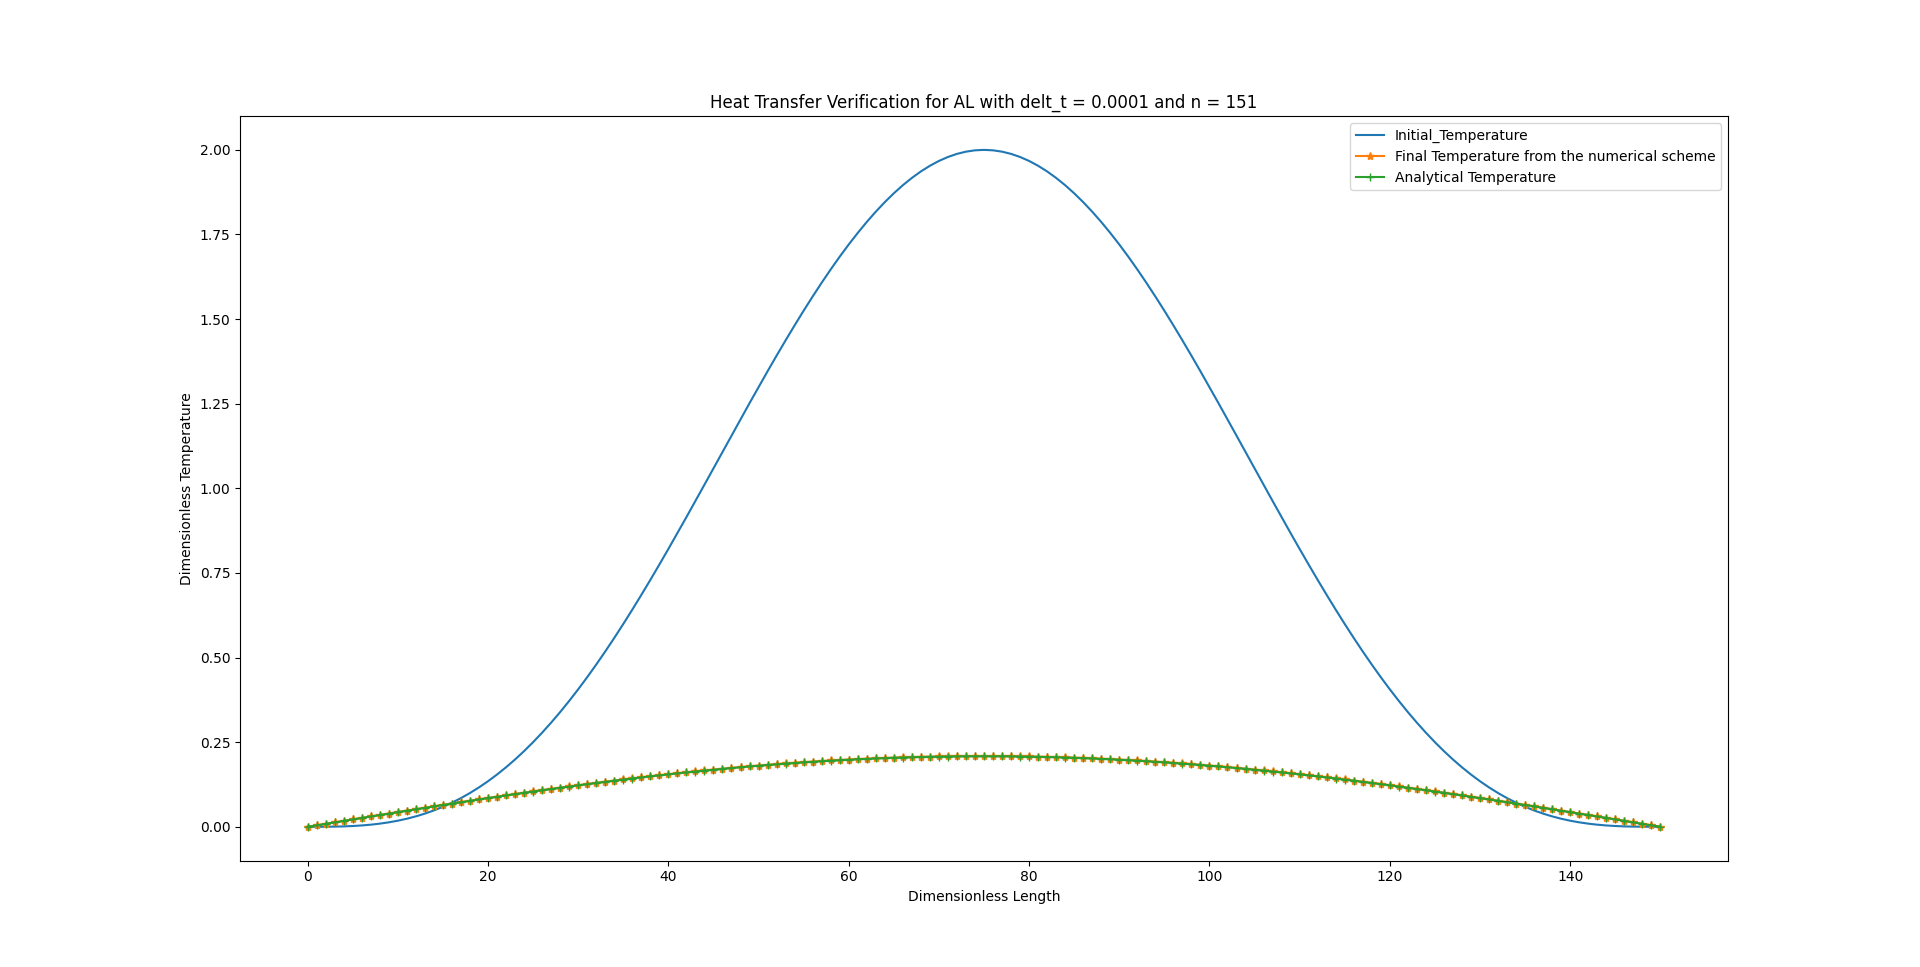
\includegraphics[width=15cm]{img/Al_Type1.png}
  \caption{Verification of the temperature distribution in Al for type I BC}
  \label{fig:Temp_Dist_in_crystal}
\end{figure}

Similarly, the figure \ref{fig:Temp_Dist_in_amorphous} shows the temperature distribution obtained from numerical and the analytical scheme for end time = 0.2 in SS304L for type 1 BC along with the initial temperature distribution. We considered 151 nodes and $\Delta t$ = 0.0001 was assumed. The root mean square error obtained using the above mentioned settings was found to be 0.090.

\begin{figure}[h]
  \centering
  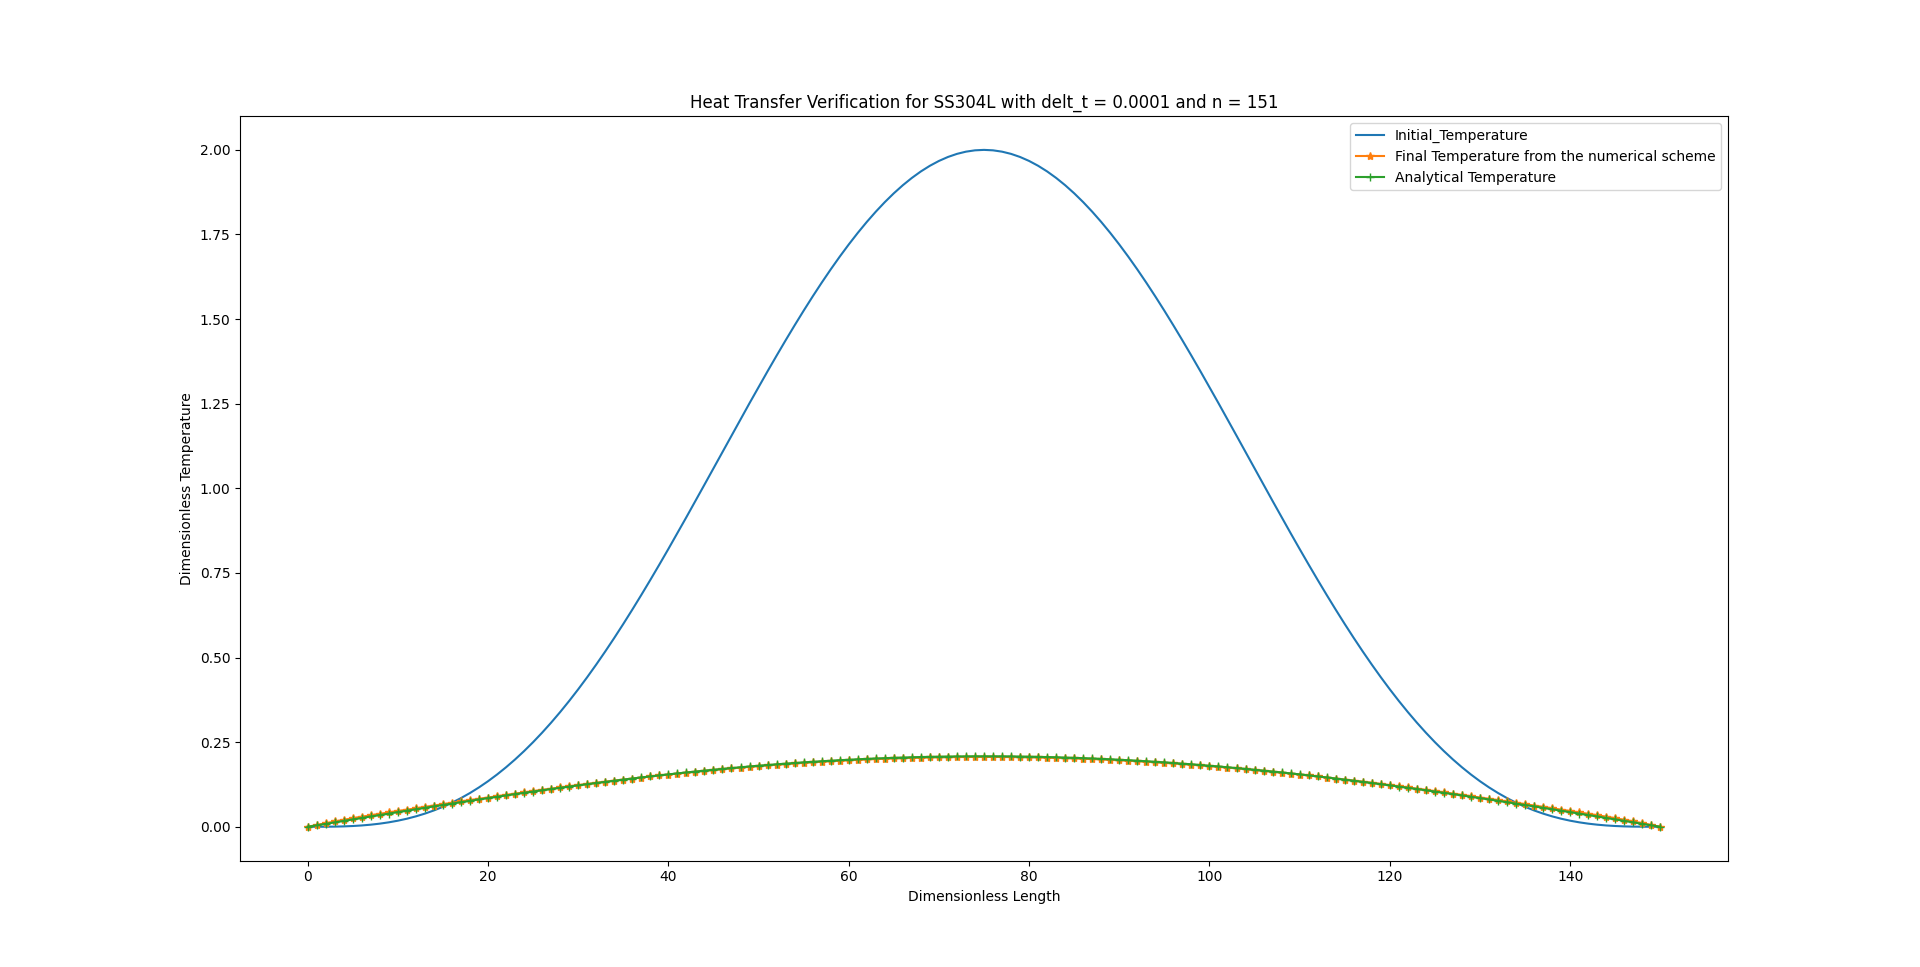
\includegraphics[width=17cm]{img/Amor_t1.png}
  \caption{Verification of the temperature distribution in SS304L for type I BC}
  \label{fig:Temp_Dist_in_amorphous}
\end{figure}
\newpage
To investigate the impact of time step ($\Delta t$) on the convergence of our solution, we conducted four separate runs, each with a different $\Delta t$ value. Throughout all runs, we maintained consistent settings, including a fixed input laser power of $1.5 \times 10^{10} \ \frac{W}{m^2}$, a total of 151 nodes, and a constant end time = 0.2. The only variable we altered was the time step.\\
In the initial run (Run 1), we set $\Delta t$ to 0.1. Subsequently, in Run 2, we reduced $\Delta t$ to 0.01. In Run 3, $\Delta t$ was further decreased to 0.001. Finally, in Run 4, we employed a much smaller $\Delta t$ of 0.0001.\\
The x-axis in our results in the figure \ref{fig:convergence_Al} represents the run count, corresponding to the specific $\Delta t$ used in each simulation run.
\begin{figure}[h]
  \centering
  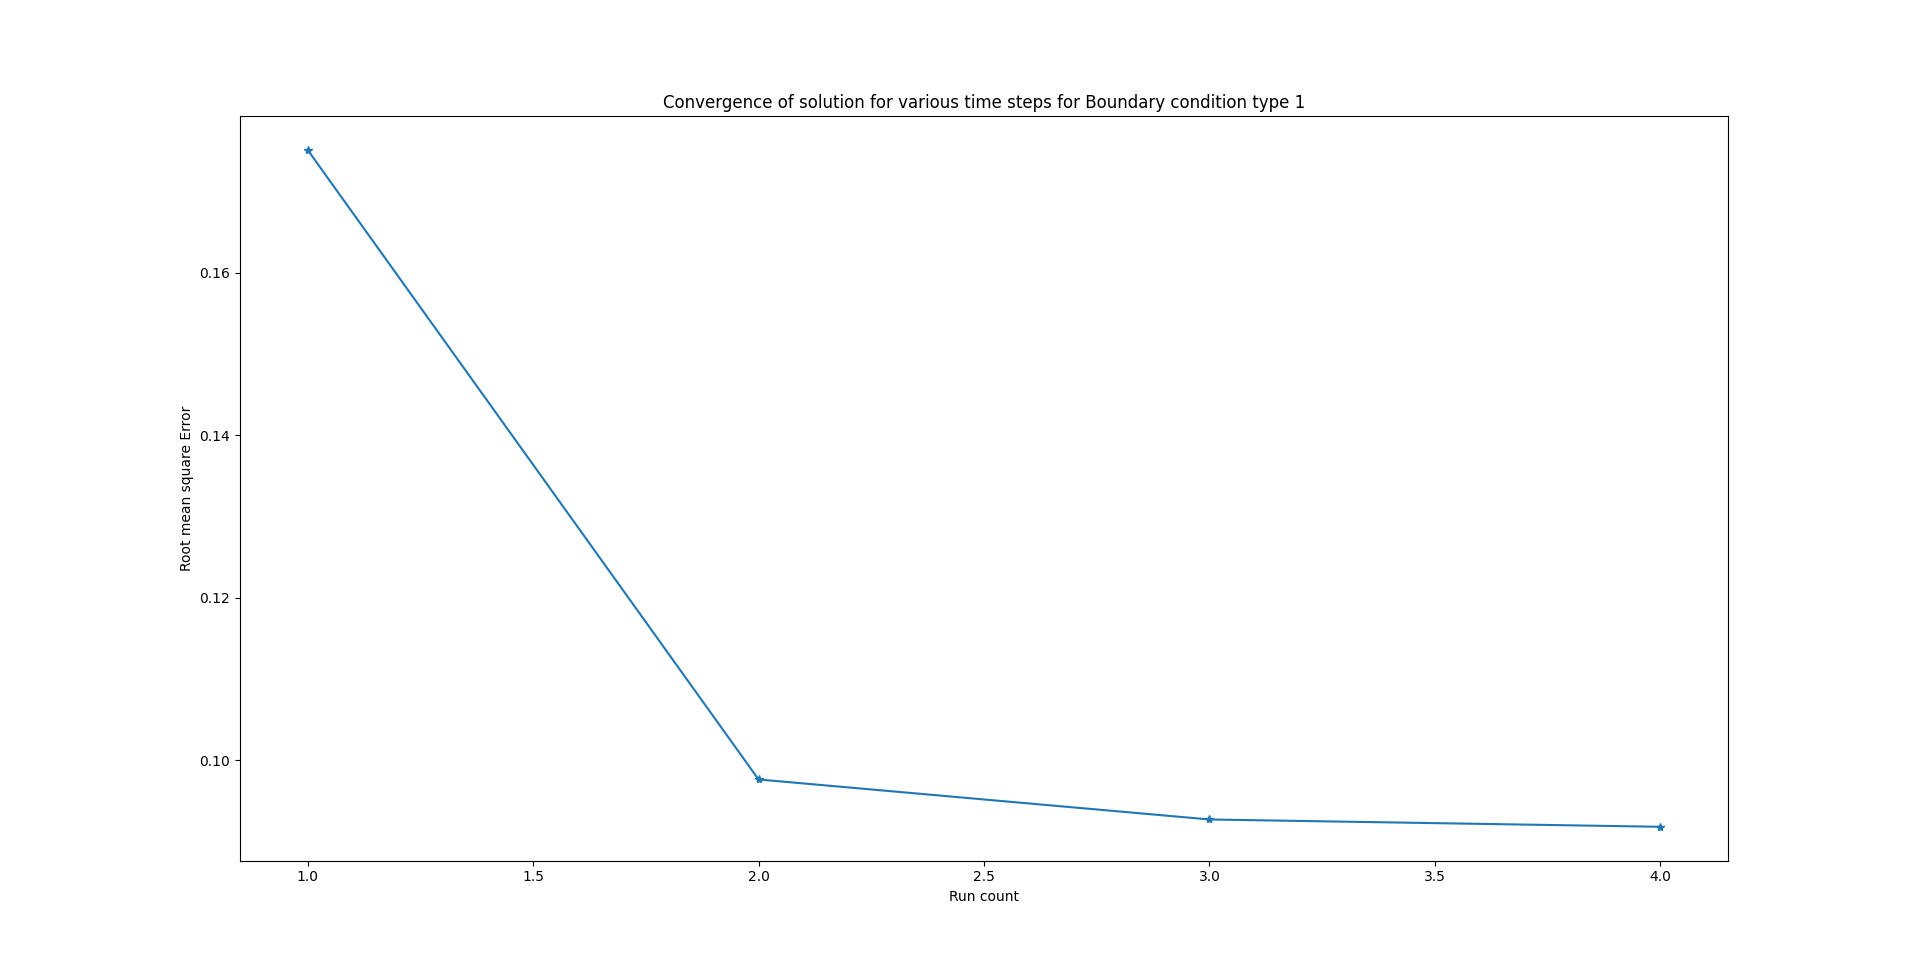
\includegraphics[width=13cm]{img/Error_convergence_for_BS1_delt_time.png}
  \caption{Convergence of the solution in Al for type I BC with variable$\Delta t$}
  \label{fig:convergence_Al}
\end{figure}

On a similar note,we conducted an examination of how the number of nodes influences the error. For this investigation, we maintained consistent settings, including a fixed input laser power of $1.5 \times 10^{10} \ \frac{W}{m^2}$, a constant $\Delta t$ of 0.001, and an end time of 0.2.  The only quantity varied was the number of nodes. The Figure \ref{fig:meshconvergence_Al} illustrates the error reduction as the number of nodes decreases. Notably, beyond 360 nodes, the error remains nearly constant.
\begin{figure}[h]
  \centering
  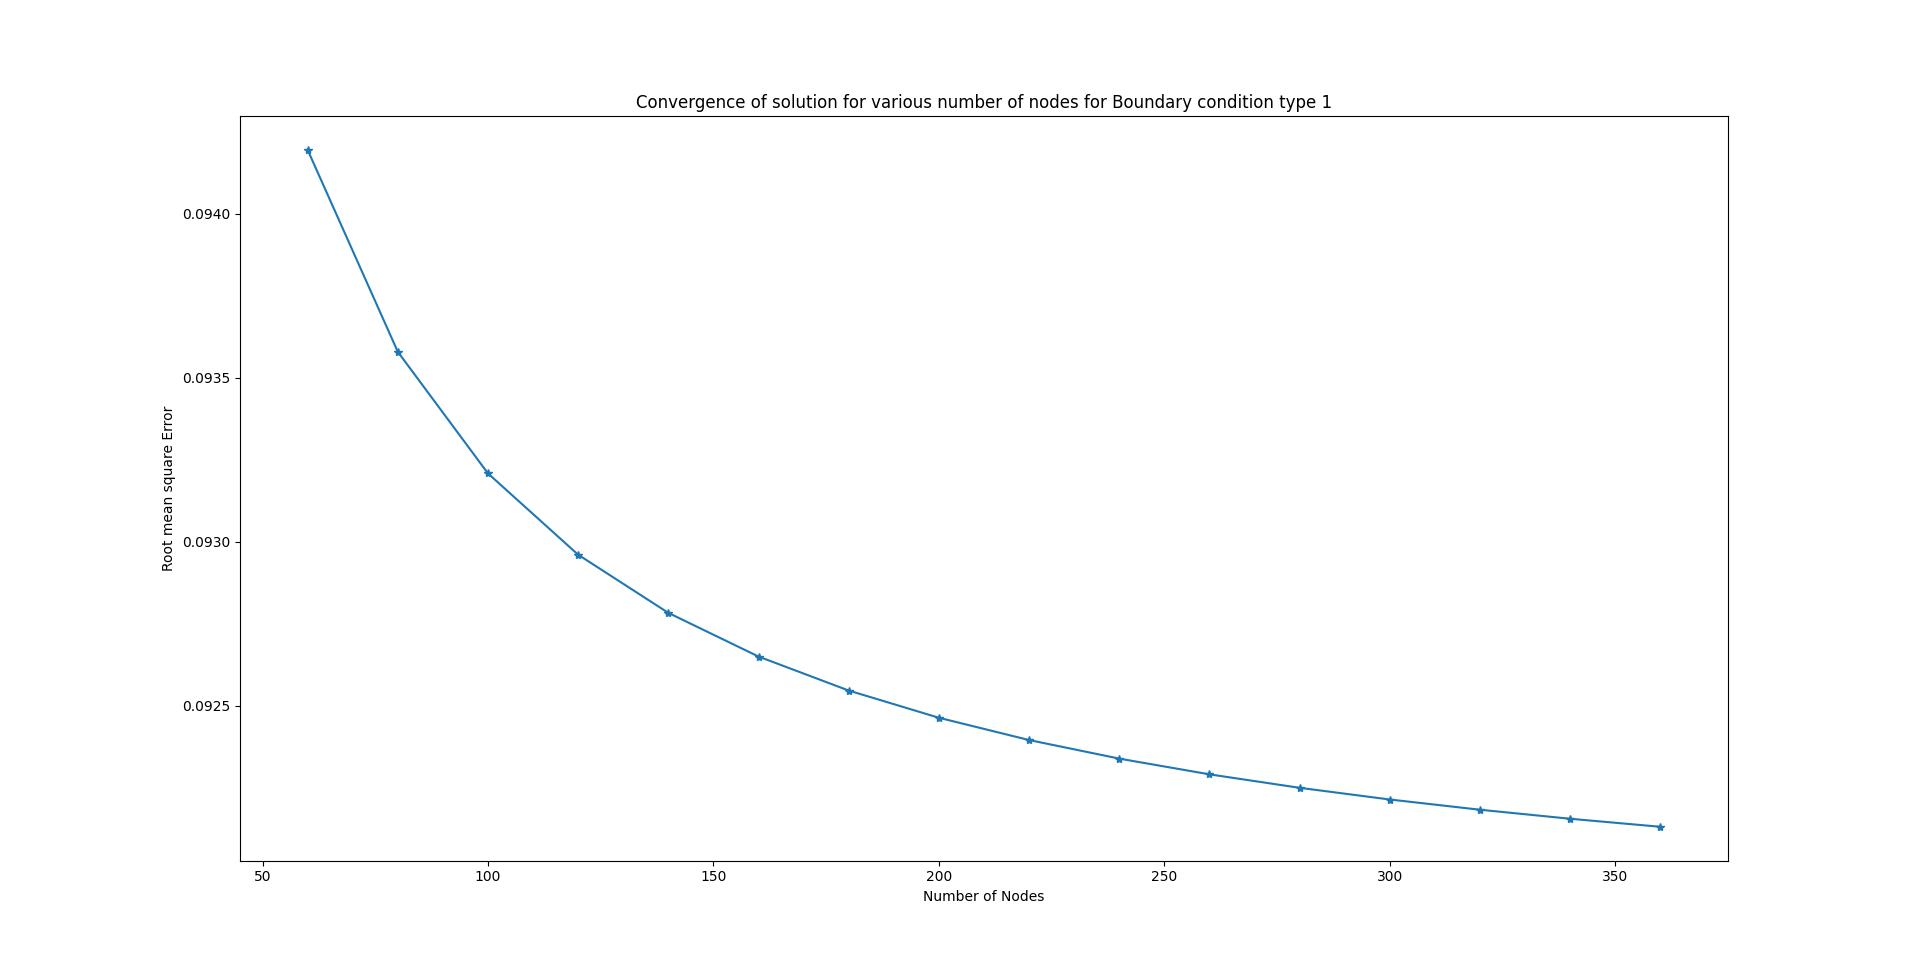
\includegraphics[width=15cm]{img/Nodal_convergence.png}
  \caption{Mesh convergence for Al using type I BC}
  \label{fig:meshconvergence_Al}
\end{figure}
\newpage
\subsection{Verification of Heat Transfer Results with Type II Boundary Conditions}
We may approximate the solution \eqref{eq:Analytical_Solution} by considering only its first term. This approximation is valid when the end time $t$ is greater than $\frac{4}{\pi^2}$, as indicated by Hancock\cite{Hancock}. In our case, with an end time of $t = 0.1$, which is less than $\frac{4}{\pi^2}$, we utilized the first 4 terms of equation \eqref{eq:Analytical_Solution}. Our choice was influenced by the observation presented in Figure \ref{fig:meshconvergence_RMS}, where it is evident that the error approaches nearly zero after adding the first 2 terms. However, for enhanced accuracy, we included the first 4 terms in the series. This error was assessed by monitoring the changes in values as new terms were added to the solution.
\begin{figure}[h]
  \centering
  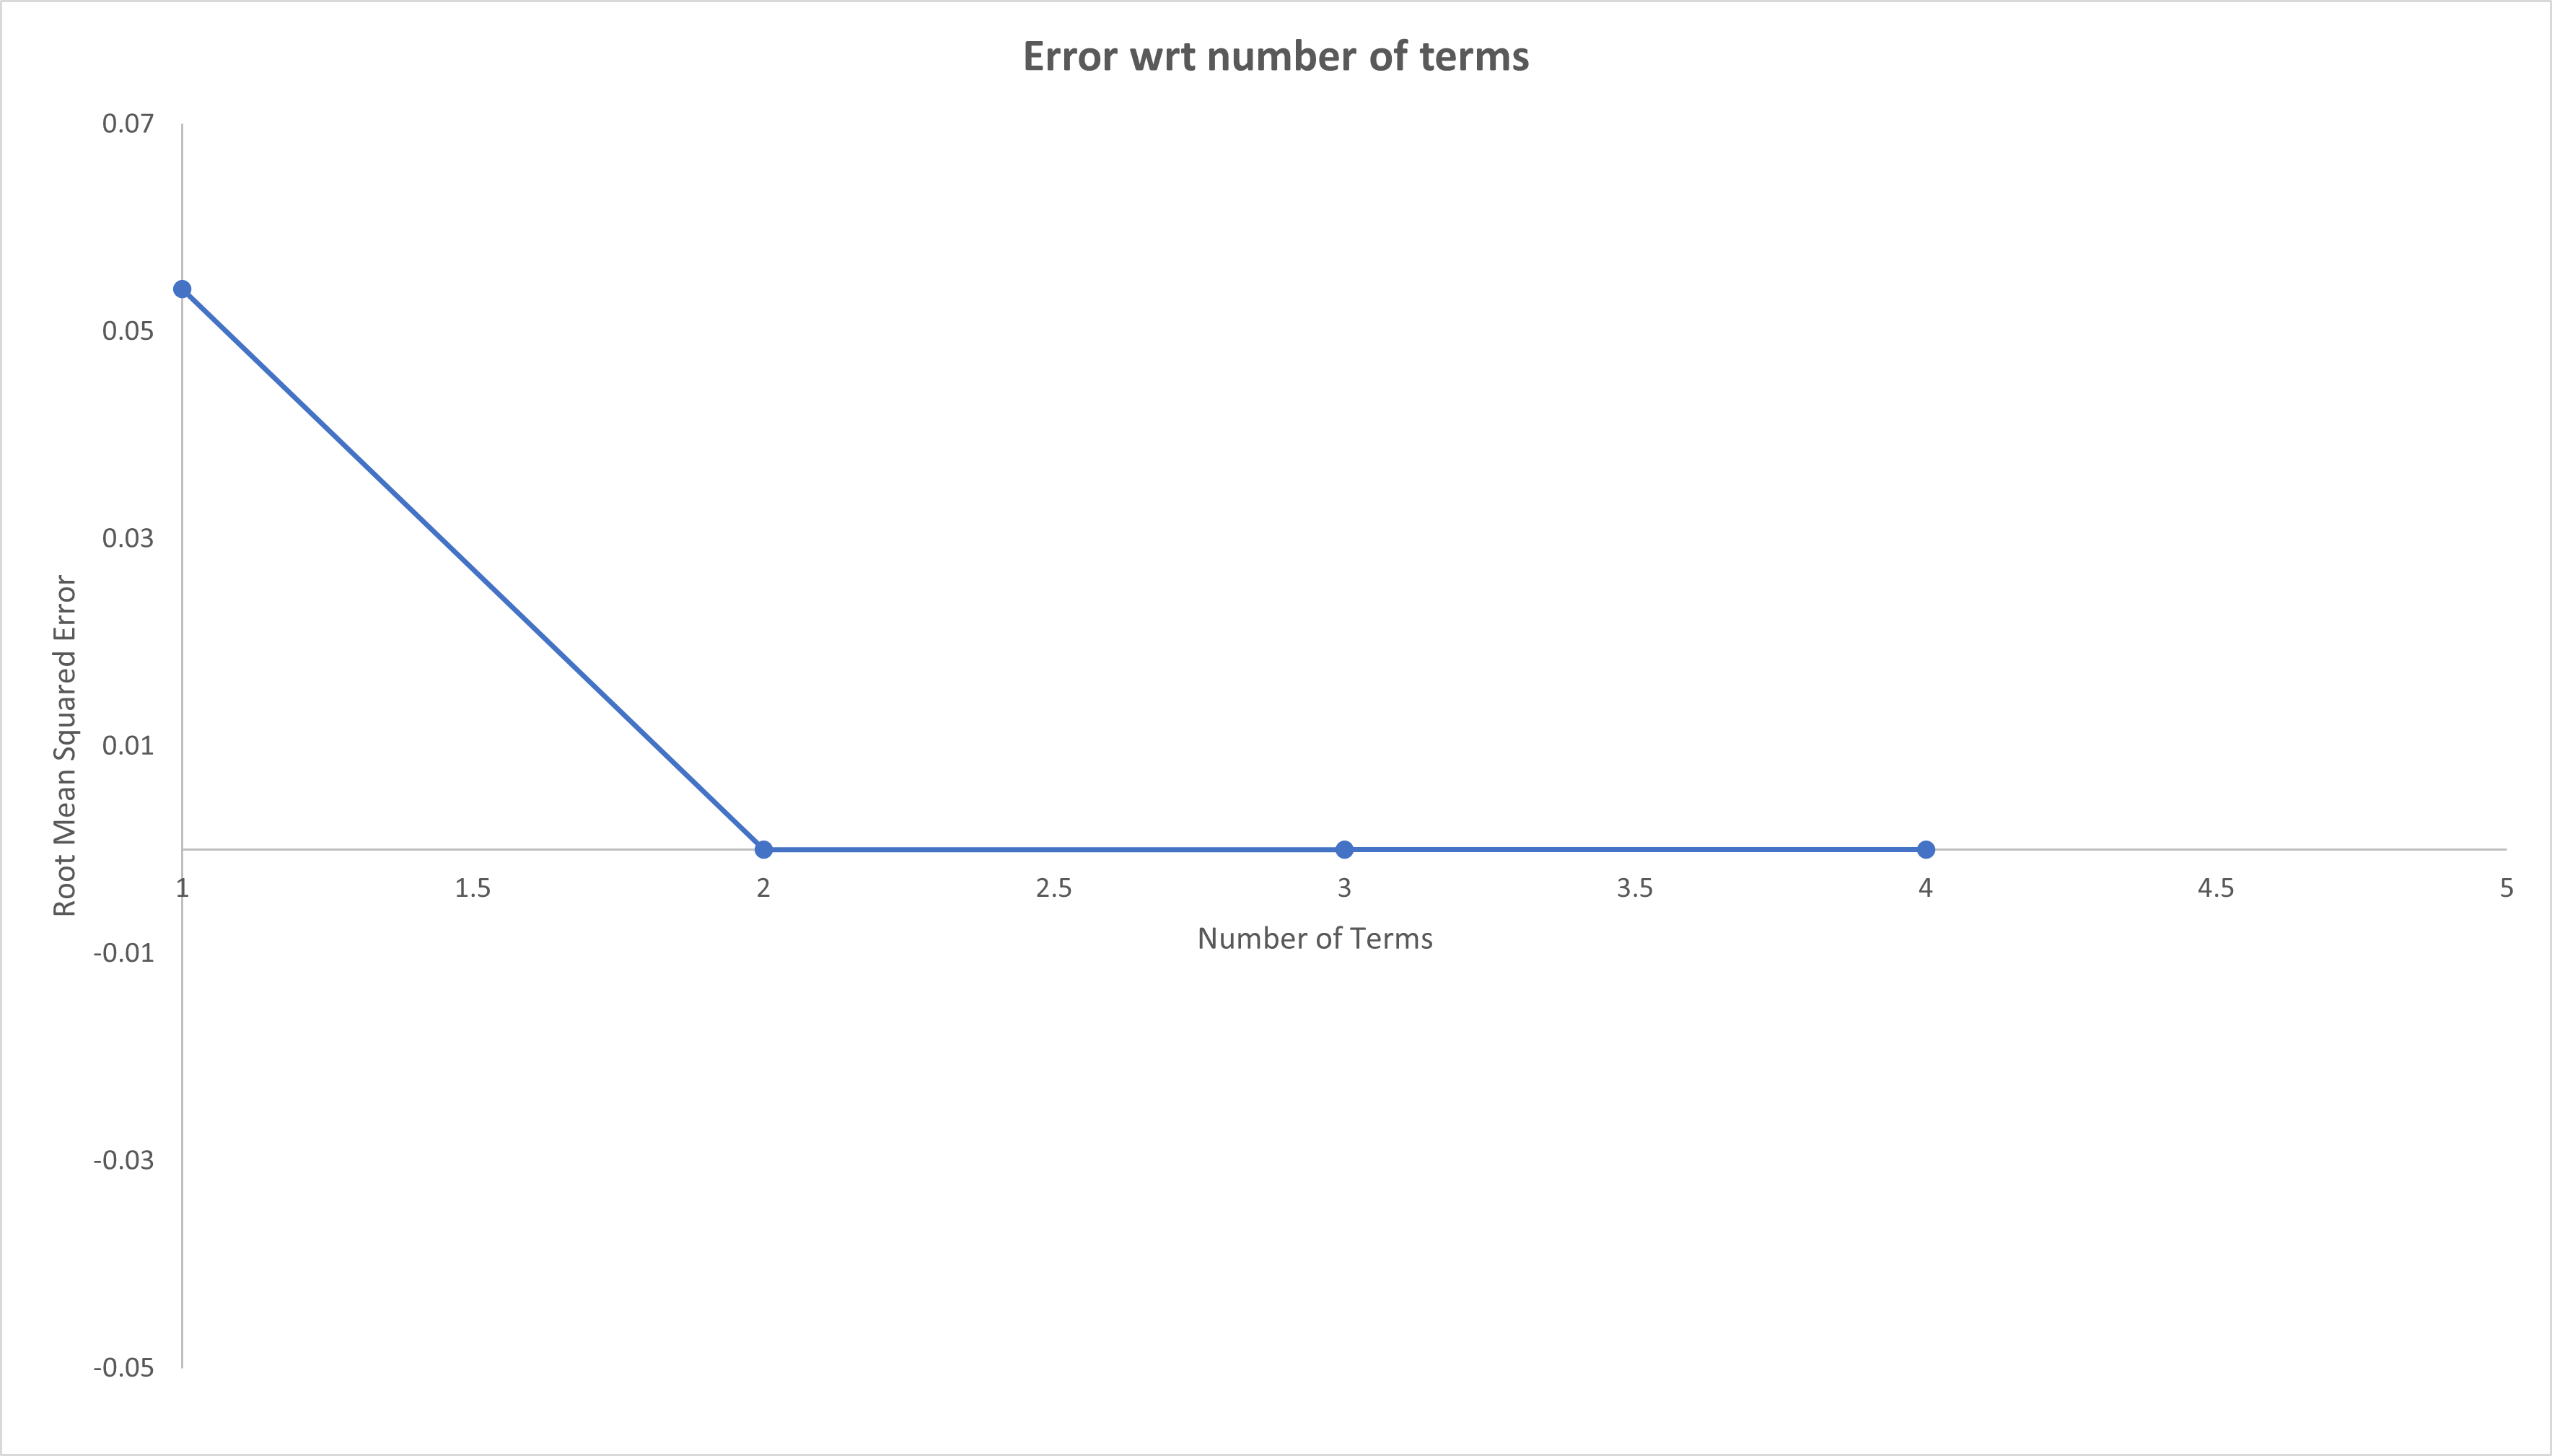
\includegraphics[width=10cm]{img/Error_in_Analytical.png}
  \caption{RMS Error Convergence with Increasing Number of Terms in Series for analytical solution with type II BC.}
  \label{fig:meshconvergence_RMS}
\end{figure}
A similar setting is employed as we used in type I BC, we employ 150 elements and $\Delta t$ was fixed to be 0.0001 with input laser power I = 1.5 x $10^{10} \ \frac{W}{m^2}$. The end time for this simulation was set to 0.1 for both the materials. The figure \ref{fig:Type2} shows the temperature distribution in AL and the figure \ref{fig:Type2SS304L} shows the temperature distribution in SS304L respectively. 
\begin{figure}[h]
  \centering
  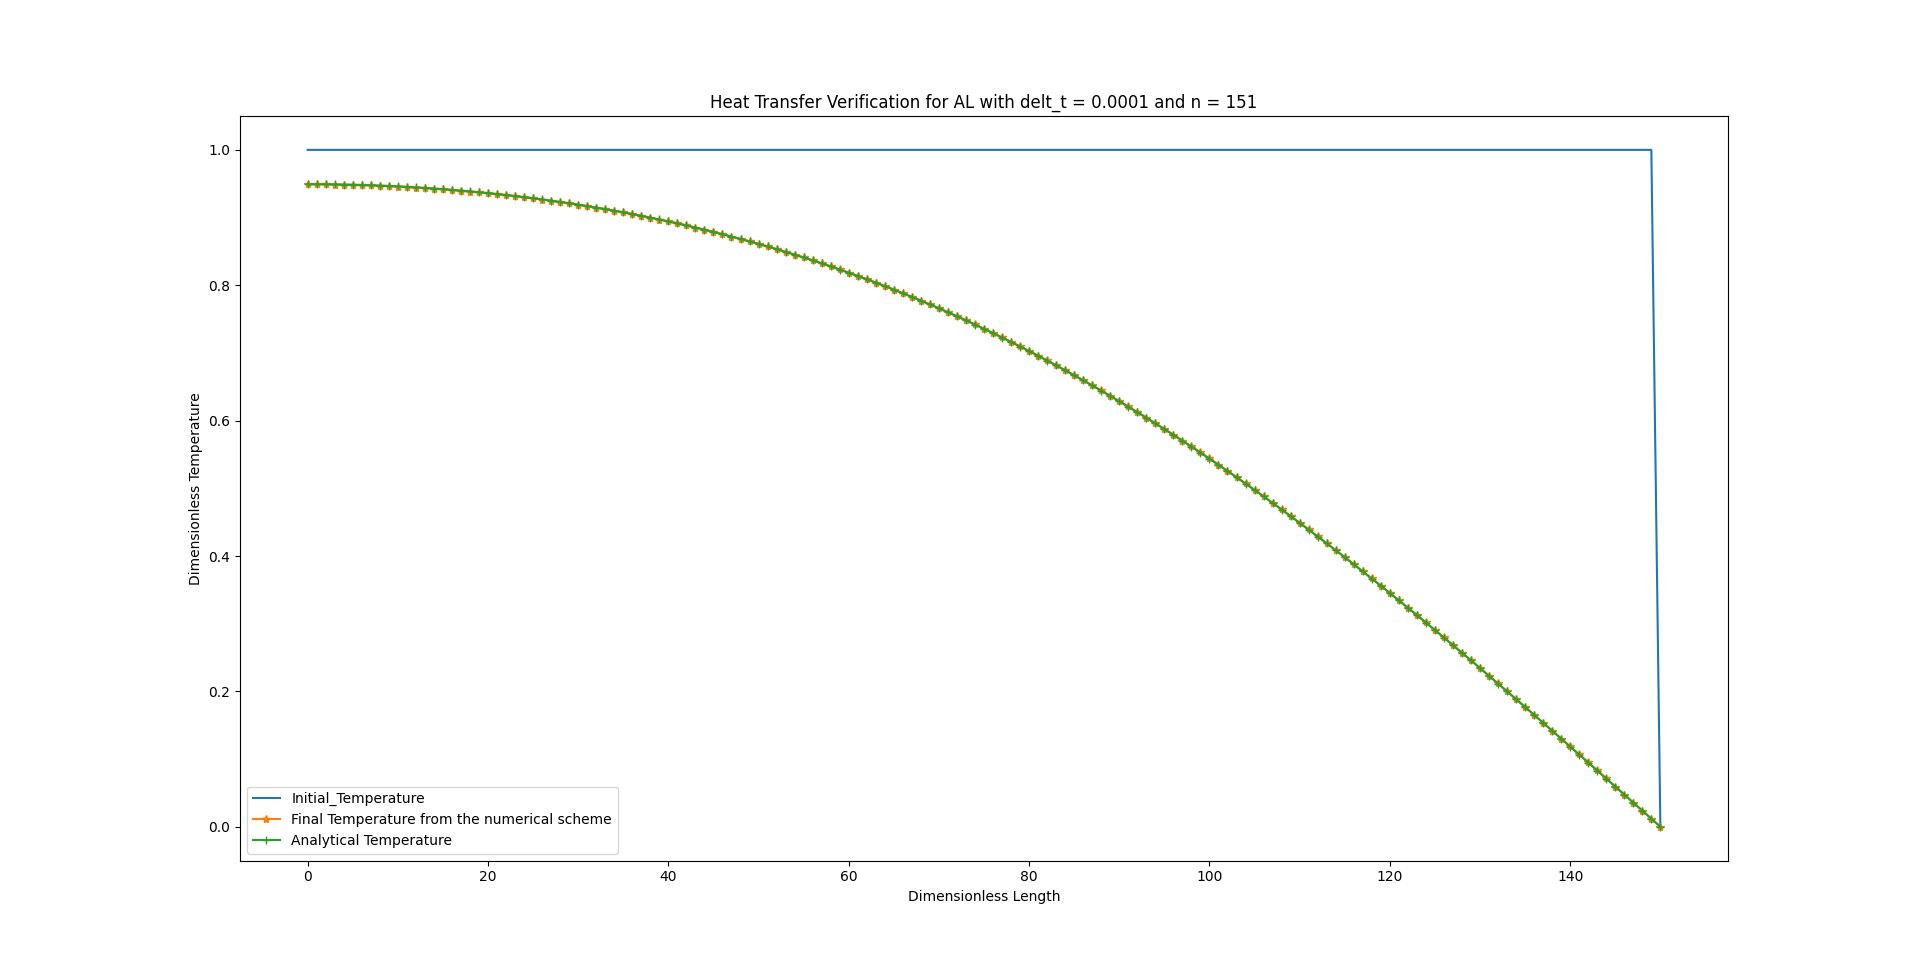
\includegraphics[width=15cm]{img/AL_type2.png}
  \caption{Verification of the temperature distribution in AL for type II BC}
  \label{fig:Type2}
\end{figure}
\begin{figure}[h]
  \centering
  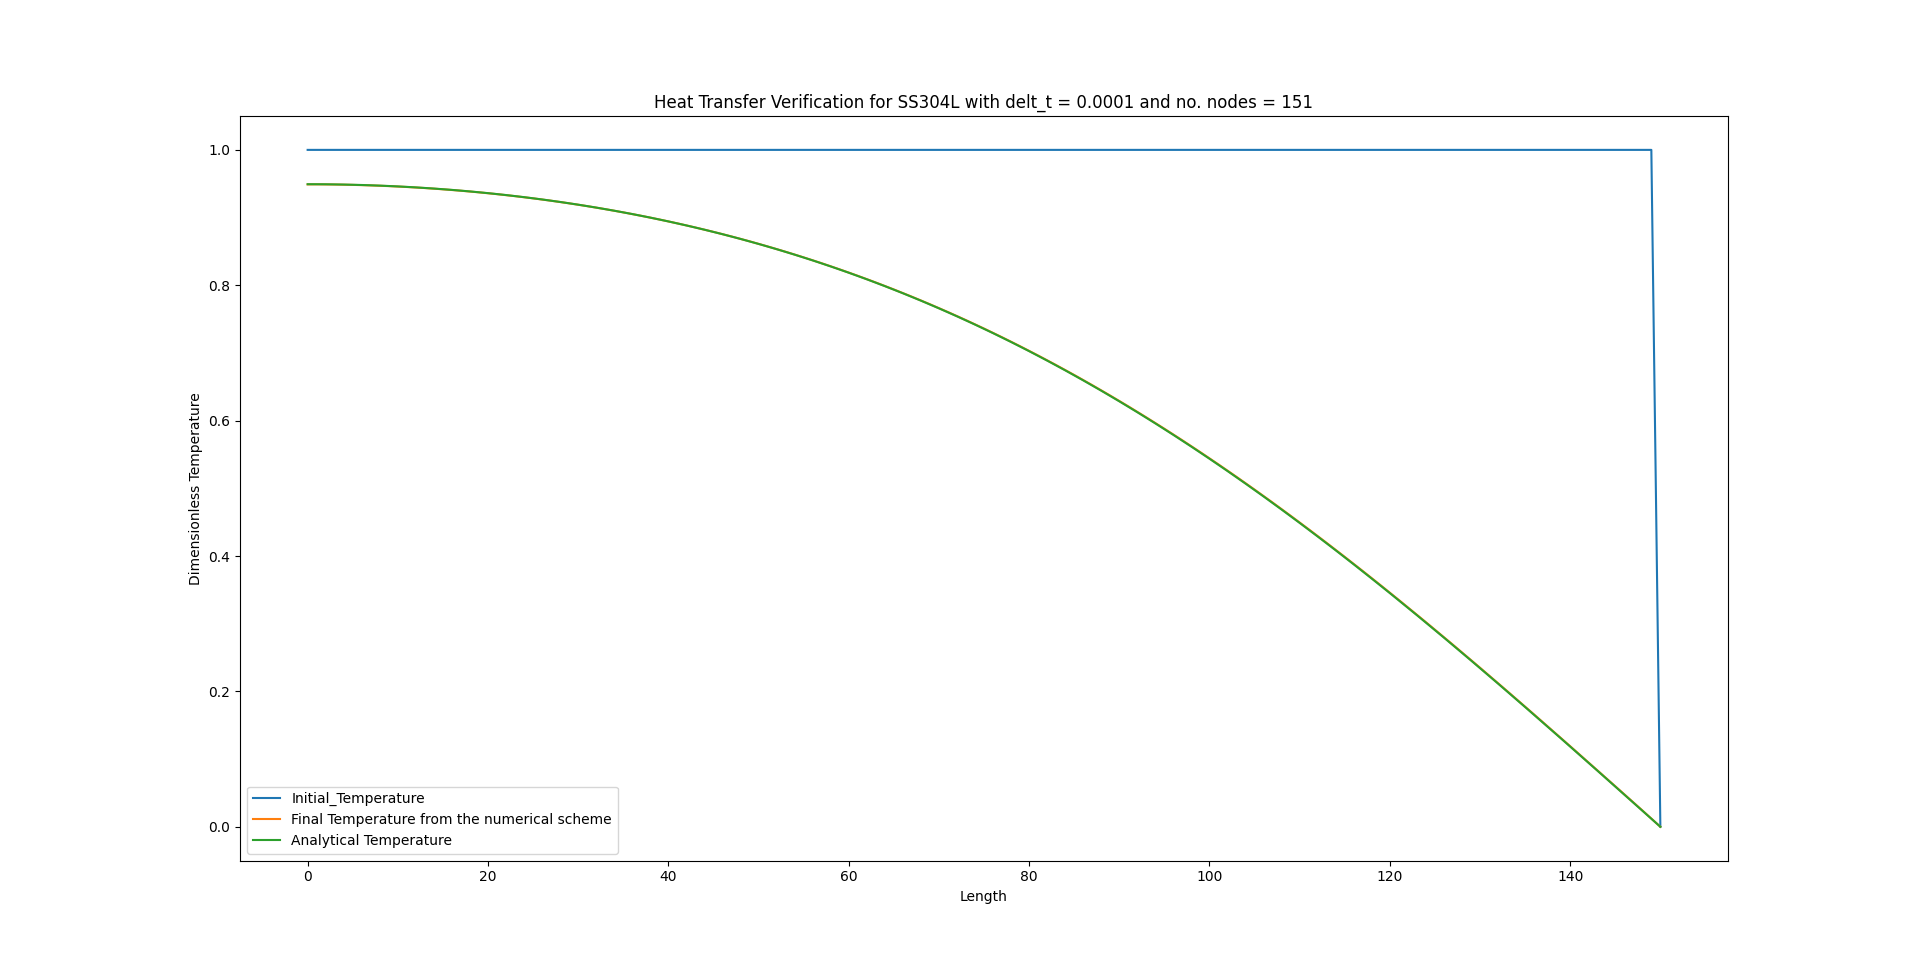
\includegraphics[width=17cm]{img/SS304_T2.png}
  \caption{Verification of the temperature distribution in SS304L for type II BC}
  \label{fig:Type2SS304L}
\end{figure}
\newpage
\subsection{Position of the Phase Change Boundary}
The analytical solution for the phase change boundary without considering the latent heat effects is given by the equation \ref{eq:melt_anal}\cite{verhoeven2003modelling}\cite{pahio(2872)_2015}.
\begin{subequations}
    \begin{align}
        R = \frac{I}{I_{\text{ref}}}\left\{2\sqrt{D}\left(\frac{t}{\pi}^{\frac{1}{2}}\right) \exp\left(-\frac{s^2}{4Dt}\right) - s \operatorname{erfc}\left(\frac{s}{2\sqrt{Dt}}\right)\right\} +T_a = 0 \label{eq:melt_anal}
    \end{align} \label{eq:analytical solution to the position}
\end{subequations}
The position of the phase change boundary is found by Euler Forward Step and Newton Raphson Scheme. For the NRS we need to find the derivative of the equation \ref{eq:melt_anal} with respect to 's'. The equation \ref{eq:derivativemelt_anal} is the derivative of equation \ref{eq:melt_anal} with respect to 's' and was found manually by hand calculations.  
\begin{subequations}
    \begin{align}
       \frac{\partial R}{\partial s} = -\frac{I}{I_{\text{ref}}}\left\{\operatorname{erfc}\left(\frac{s}{2\sqrt{Dt}}\right)\right\} \label{eq:derivativemelt_anal}
    \end{align}
\end{subequations}

Using the equations \ref{eq:melt_anal} and \ref{eq:derivativemelt_anal} we have plotted the analytical solution in figures \ref{fig:phasechange} to \ref{fig:AL_Latenthear} for the verification of the position of the phase front in Al and SS304L for each time step.
\begin{figure}[h]
  \centering
  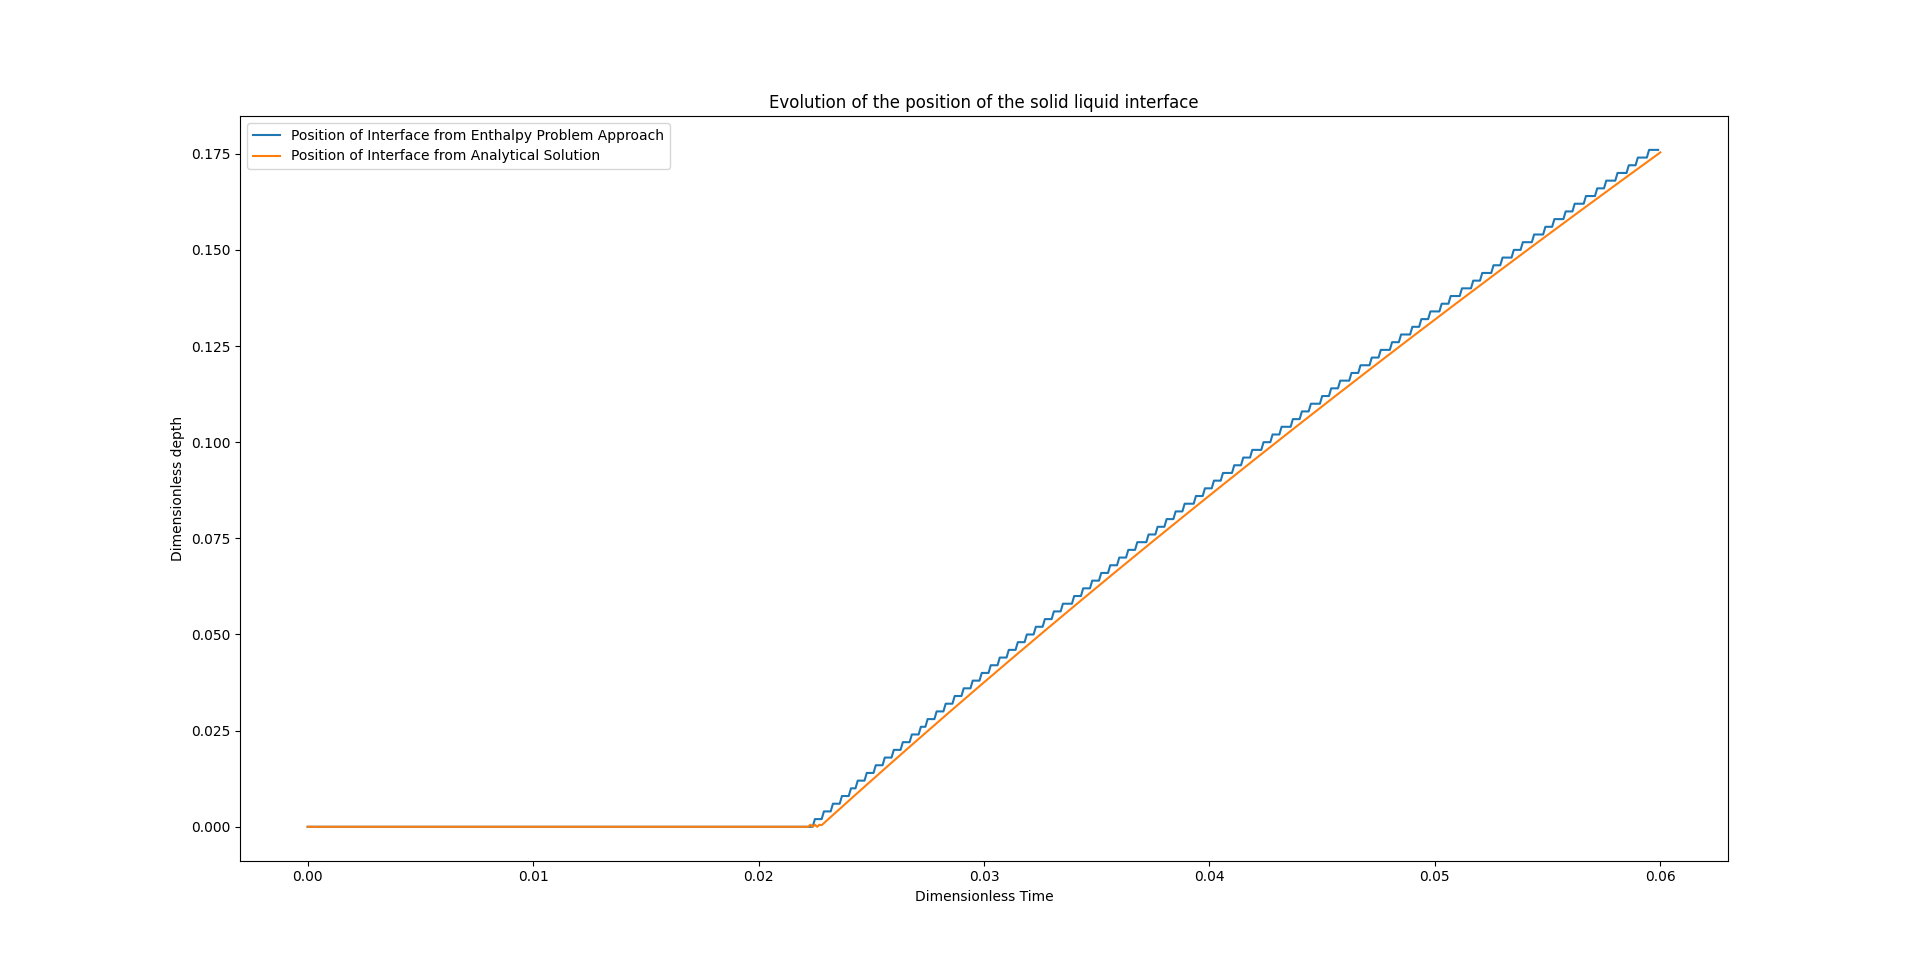
\includegraphics[width=17cm]{img/Evolution_of_the_mushy_zone_for_crystalline_material_under_301_nodes.png}
  \caption{Phase Change Boundary Evolution (Al, No Latent Heat, 301 Nodes)}
  \label{fig:phasechange}
\end{figure}

\begin{figure}[h]
  \centering
  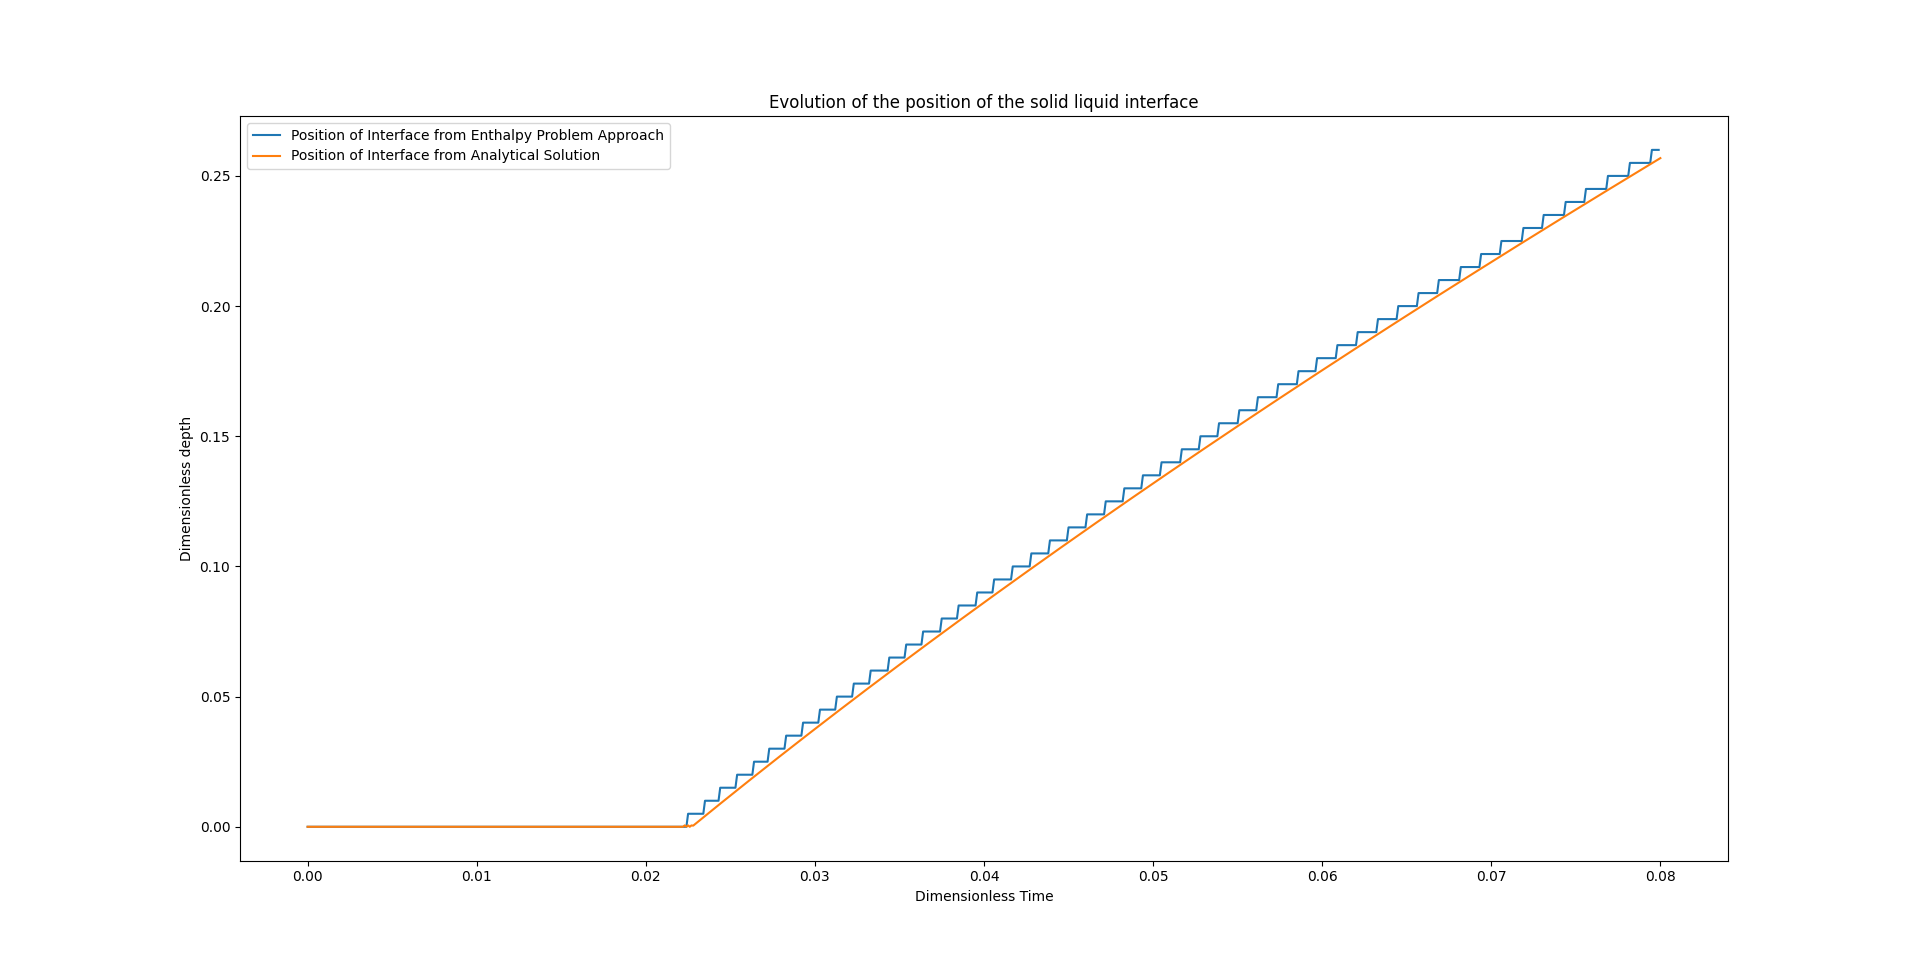
\includegraphics[width=15cm]{img/Evolution_of_the_Mushy_Zone.png}
  \caption{Phase Change Boundary Evolution (Al, No Latent Heat, 201 Nodes)}
  \label{fig:201_Nodes_phasechange}
\end{figure}

\begin{figure}[h]
  \centering
  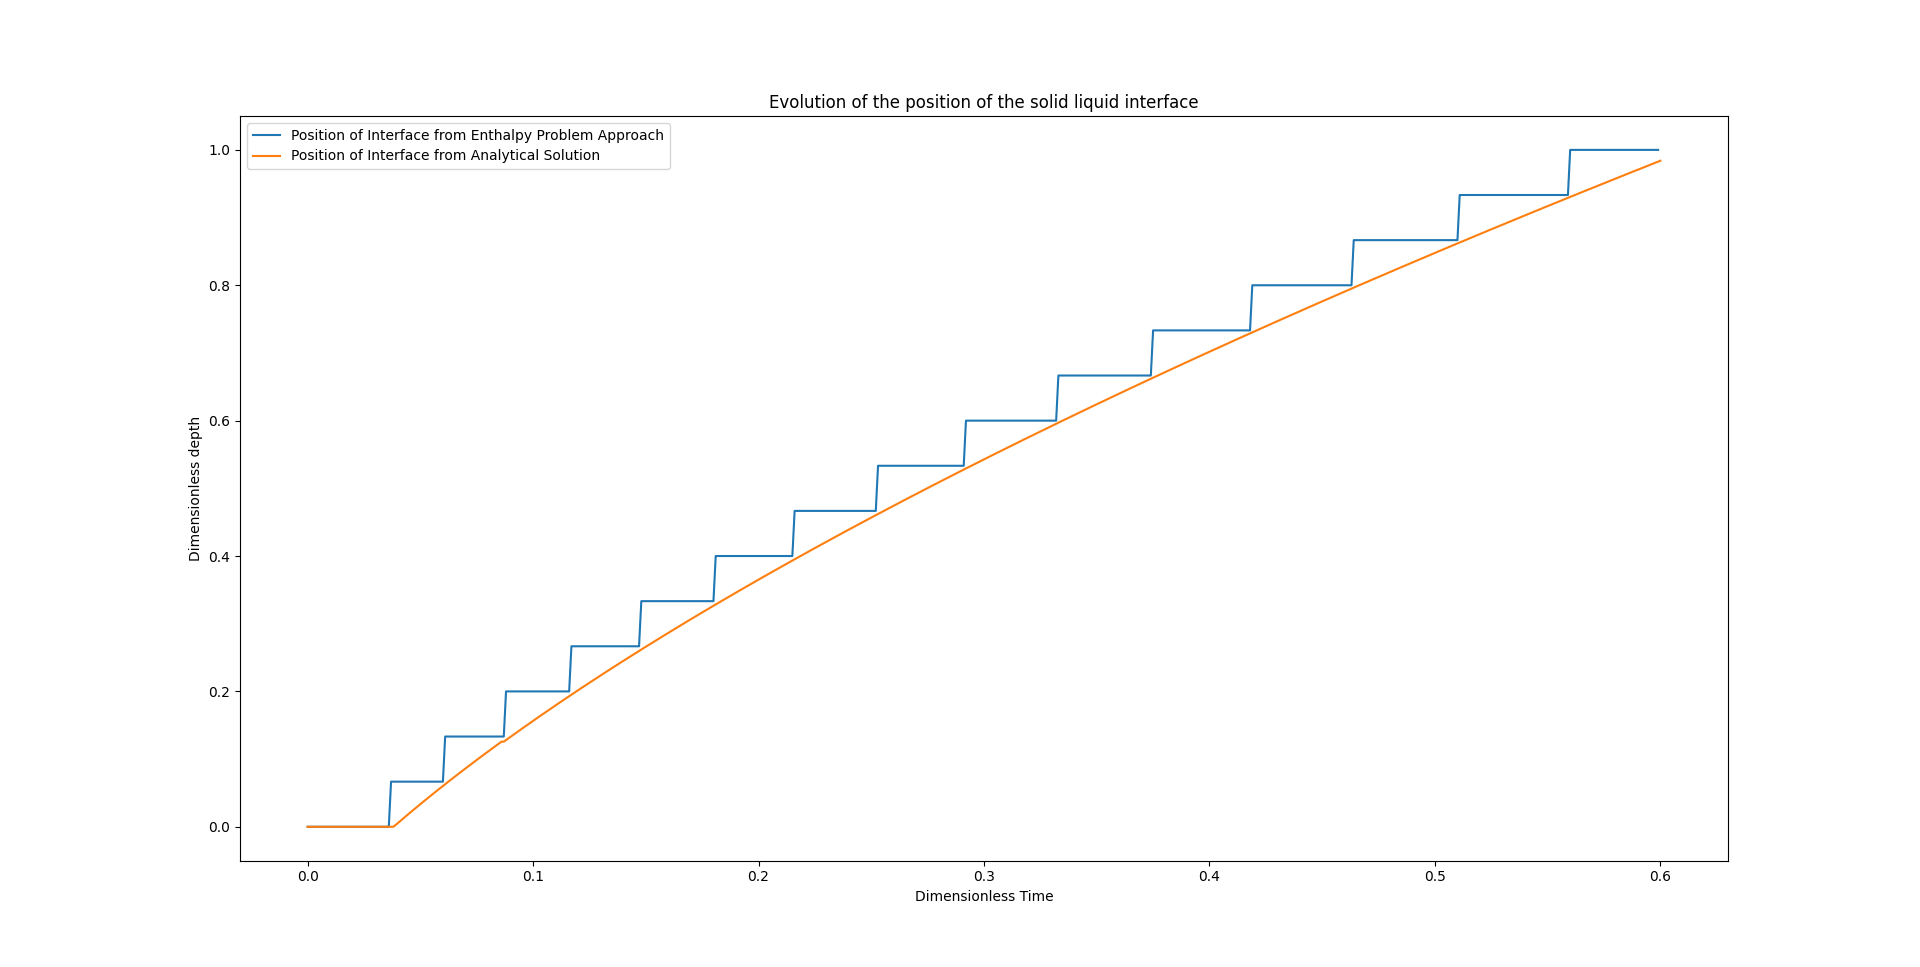
\includegraphics[width=15cm]{img/Amorphous_No_Latent_Heat_151_nodes.png}
  \caption{Phase Change Boundary Evolution (SS304L, No Latent Heat, 151 Nodes)}
  \label{fig:Amor_phasechange}
\end{figure}

\begin{figure}[h]
  \centering
  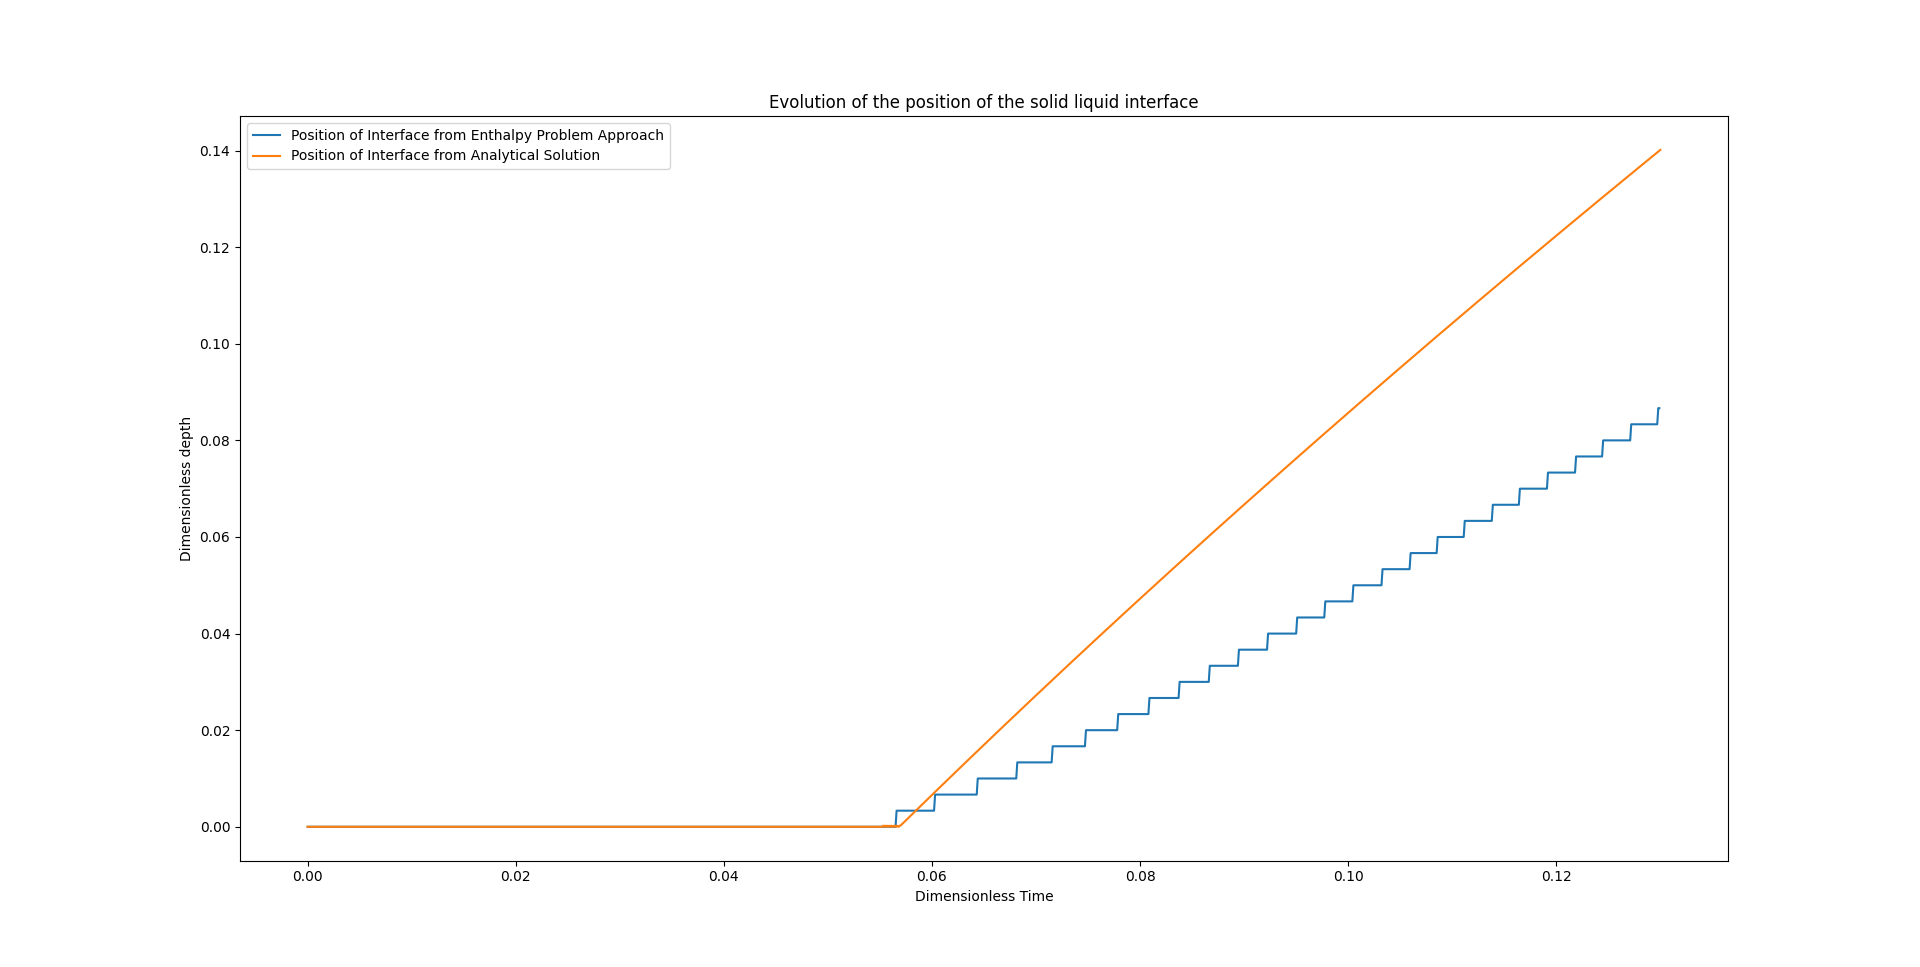
\includegraphics[width=15cm]{img/Evolution_of_mushy_zone_when_the_latent_heat_is_on.png}
  \caption{Phase Change Boundary Evolution (Al, 151 Nodes ,considering Latent Heat effects)}
  \label{fig:AL_Latenthear}
\end{figure}
\newpage
 In the in figures \ref{fig:phasechange} to \ref{fig:AL_Latenthear} we observe the staircase-like behaviour which was also observed by Ben Hills\cite{Hills_2016} in his paper. It takes time for the interface to travel through an element where tracking of the interface is impossible due to absence of nodes within the elements. The author J.C.J. Verhoeven in his paper \cite{verhoeven2003modelling} has mentioned two techniques to overcome this issue. One method is to use finer mesh (which is already done in our work) and the other is a method suggested by Tacke\cite{Tacke1985DiscretizationOT} (which we did not use in this project).\\
 We observe the impact of a finer mesh by comparing the results in Figure \ref{fig:phasechange} (301 nodes) with Figure \ref{fig:201_Nodes_phasechange} (201 nodes). The influence of considering latent heat on the interface's evolution is evident in Figure \ref{fig:AL_Enthalpy_Temperature_Latent_Heat}, while Figures \ref{fig:AL_Enthalpy_Temperature} and \ref{fig:AL_Enthalpy_Temperature_Latent_Heat} illustrate the effect of latent heat on enthalpy evolution at node 1. In our Python simulation, node 1 corresponds to the node just below the one where heat flux is applied. The figure \ref{fig:AL_Enthalpy_Temperature_Latent_Heat} and \ref{fig:SS304L_Enthalpy_Temperature_Latent_Heat} also provides a visual verification for retention of material characteristic in our material model for crystalline and amorphous material respectively. 
\begin{figure}[h]
  \centering
  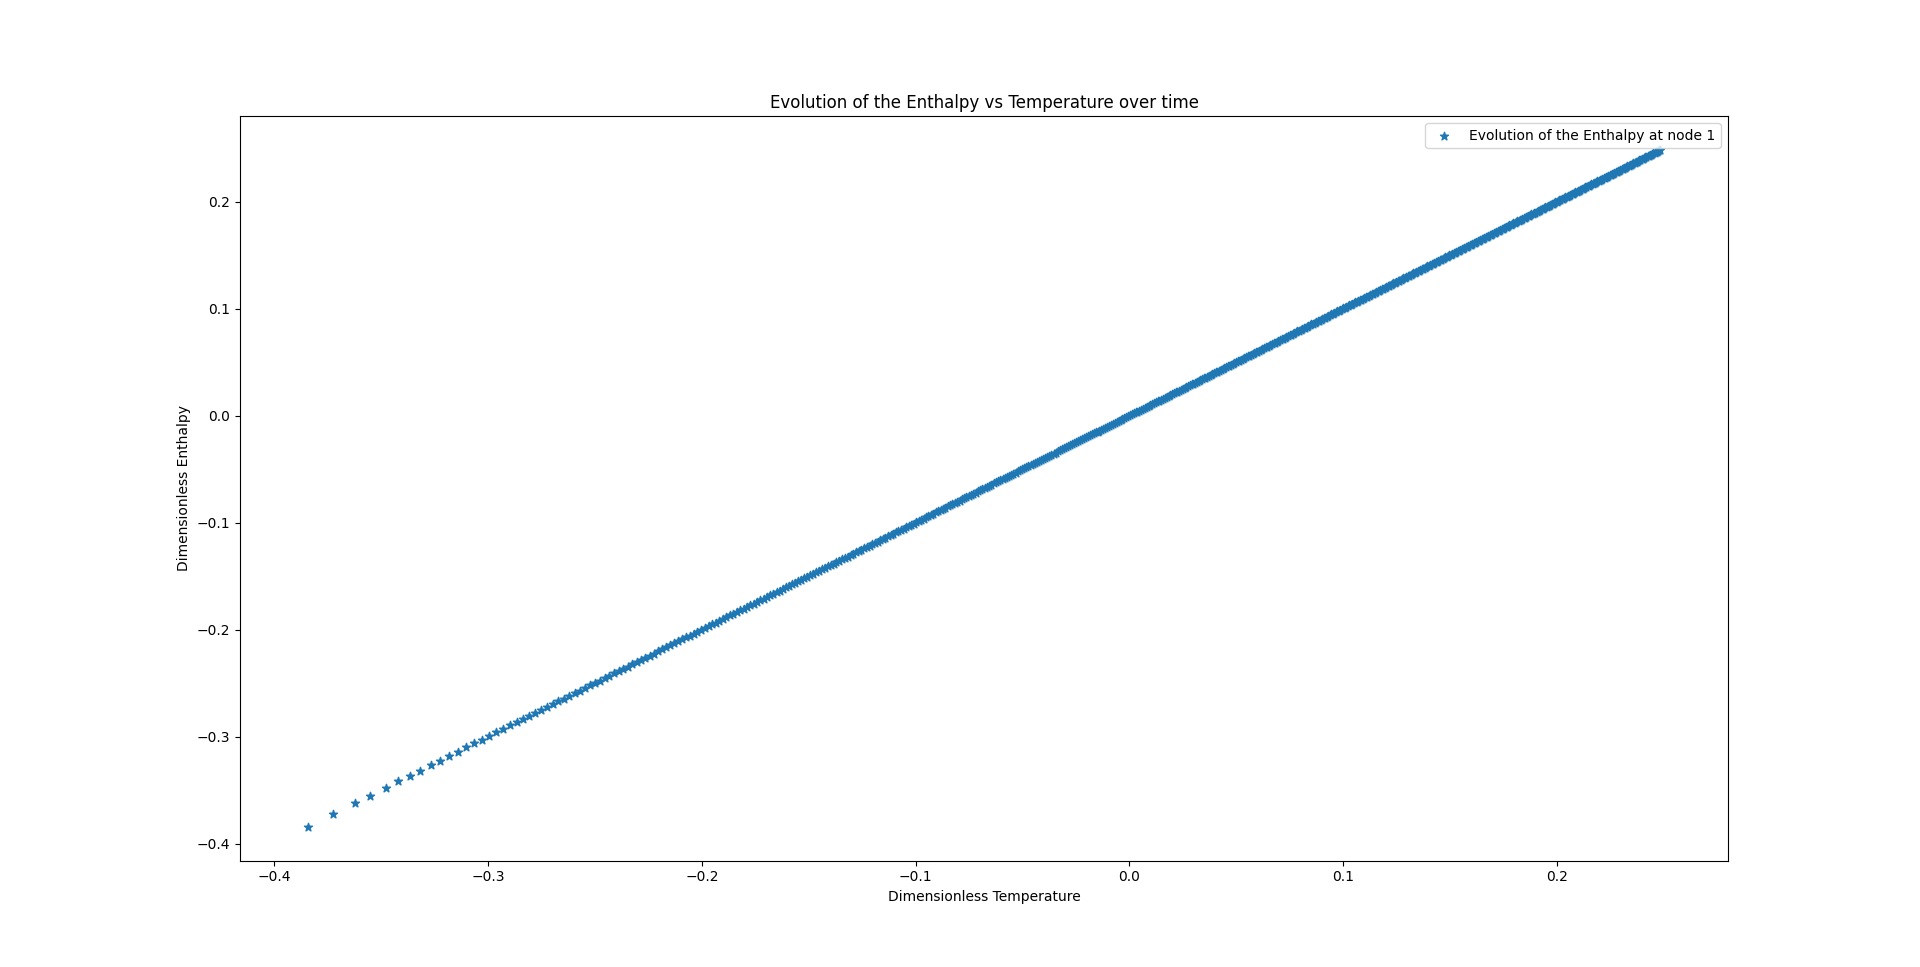
\includegraphics[width=15cm]{img/Evolution_of_Enthalpy_at_node_2_Crystalline_materials_no_latent_heat.png}
  \caption{Enthlapy vs Temperature (Al, 151 Nodes ,no Latent Heat effects considered)}
  \label{fig:AL_Enthalpy_Temperature}
\end{figure}

\begin{figure}[h]
  \centering
  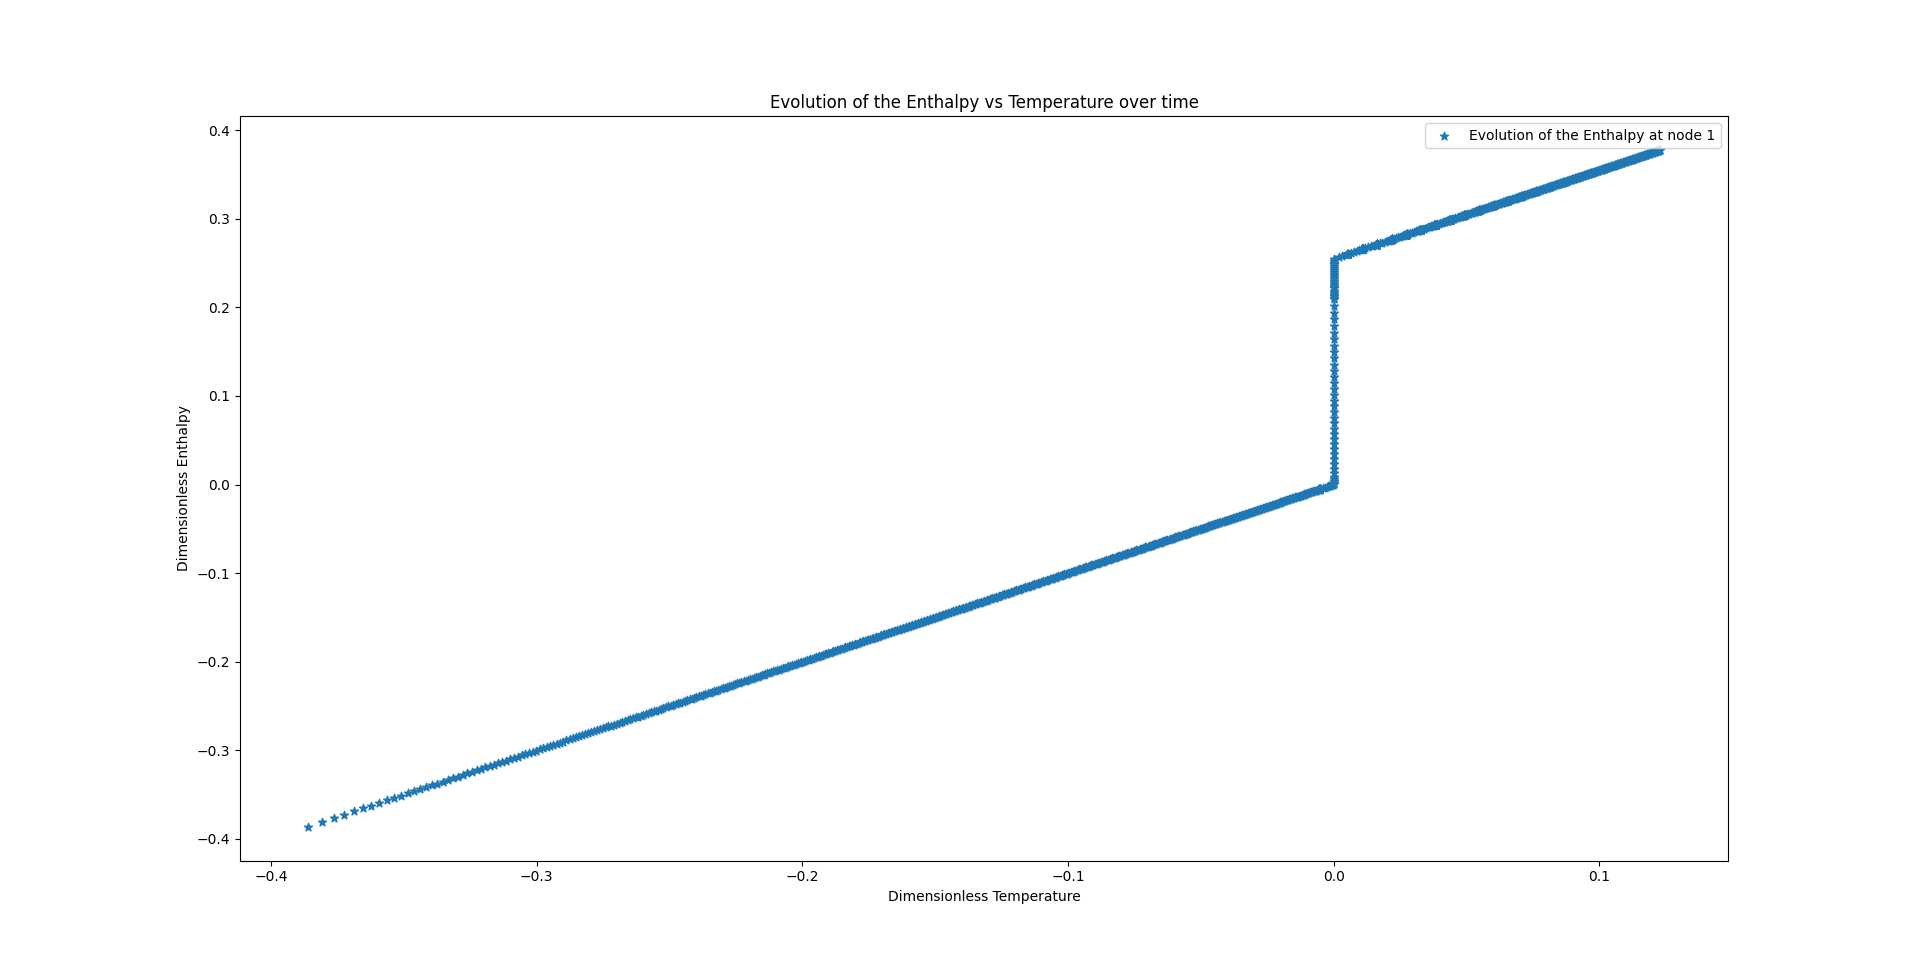
\includegraphics[width=15cm]{img/Temperature_vs_enthalpy_with_latent_heat_crystalline.png}
  \caption{Enthlapy vs Temperature (Al, 301 Nodes ,considering Latent Heat effects)}
  \label{fig:AL_Enthalpy_Temperature_Latent_Heat}
  
  \centering
  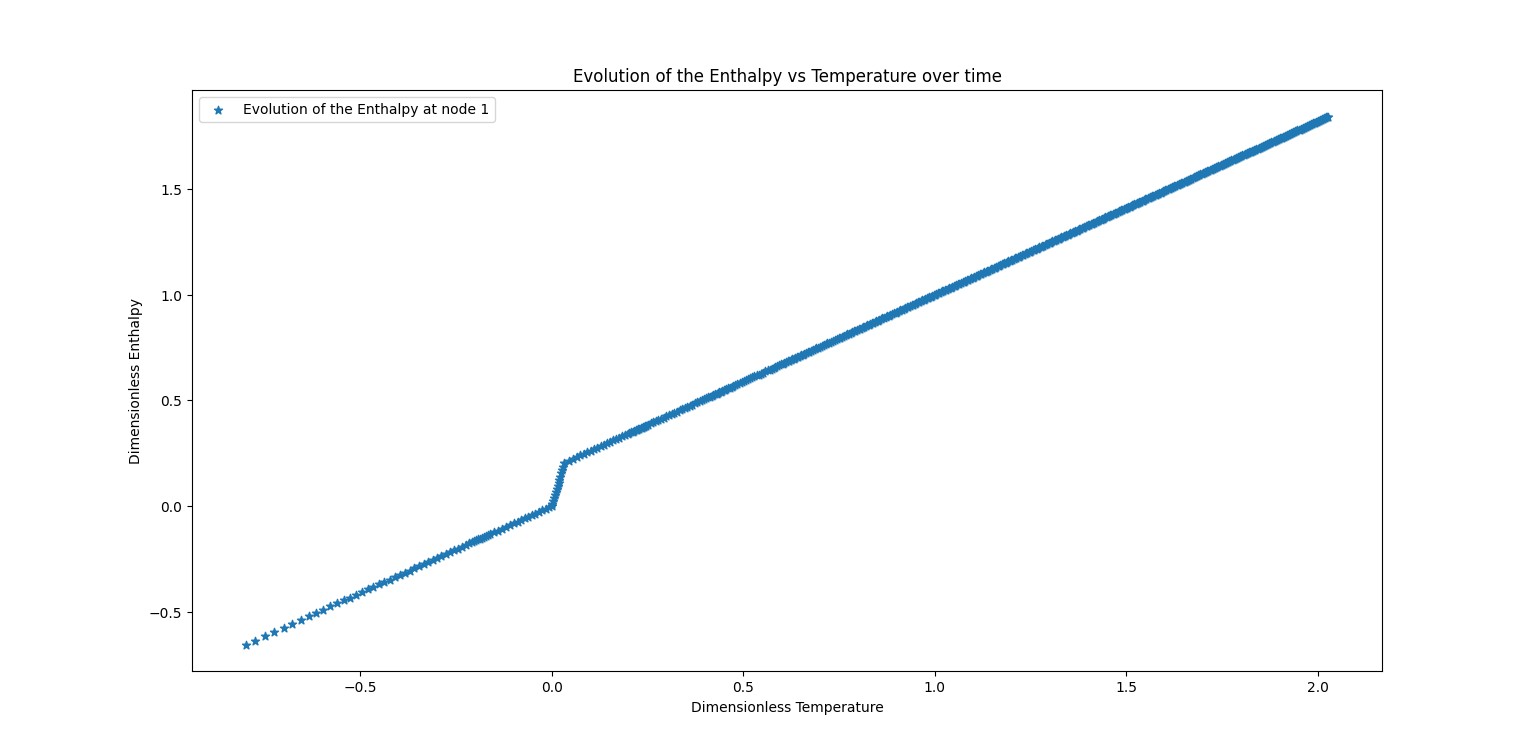
\includegraphics[width=15cm]{img/H_Tfor_amorphous.png}
  \caption{Enthlapy vs Temperature (SS304L, 151 Nodes ,considering Latent Heat effects)}
  \label{fig:SS304L_Enthalpy_Temperature_Latent_Heat}
  
\end{figure}

\begin{figure}[h]
\centering
  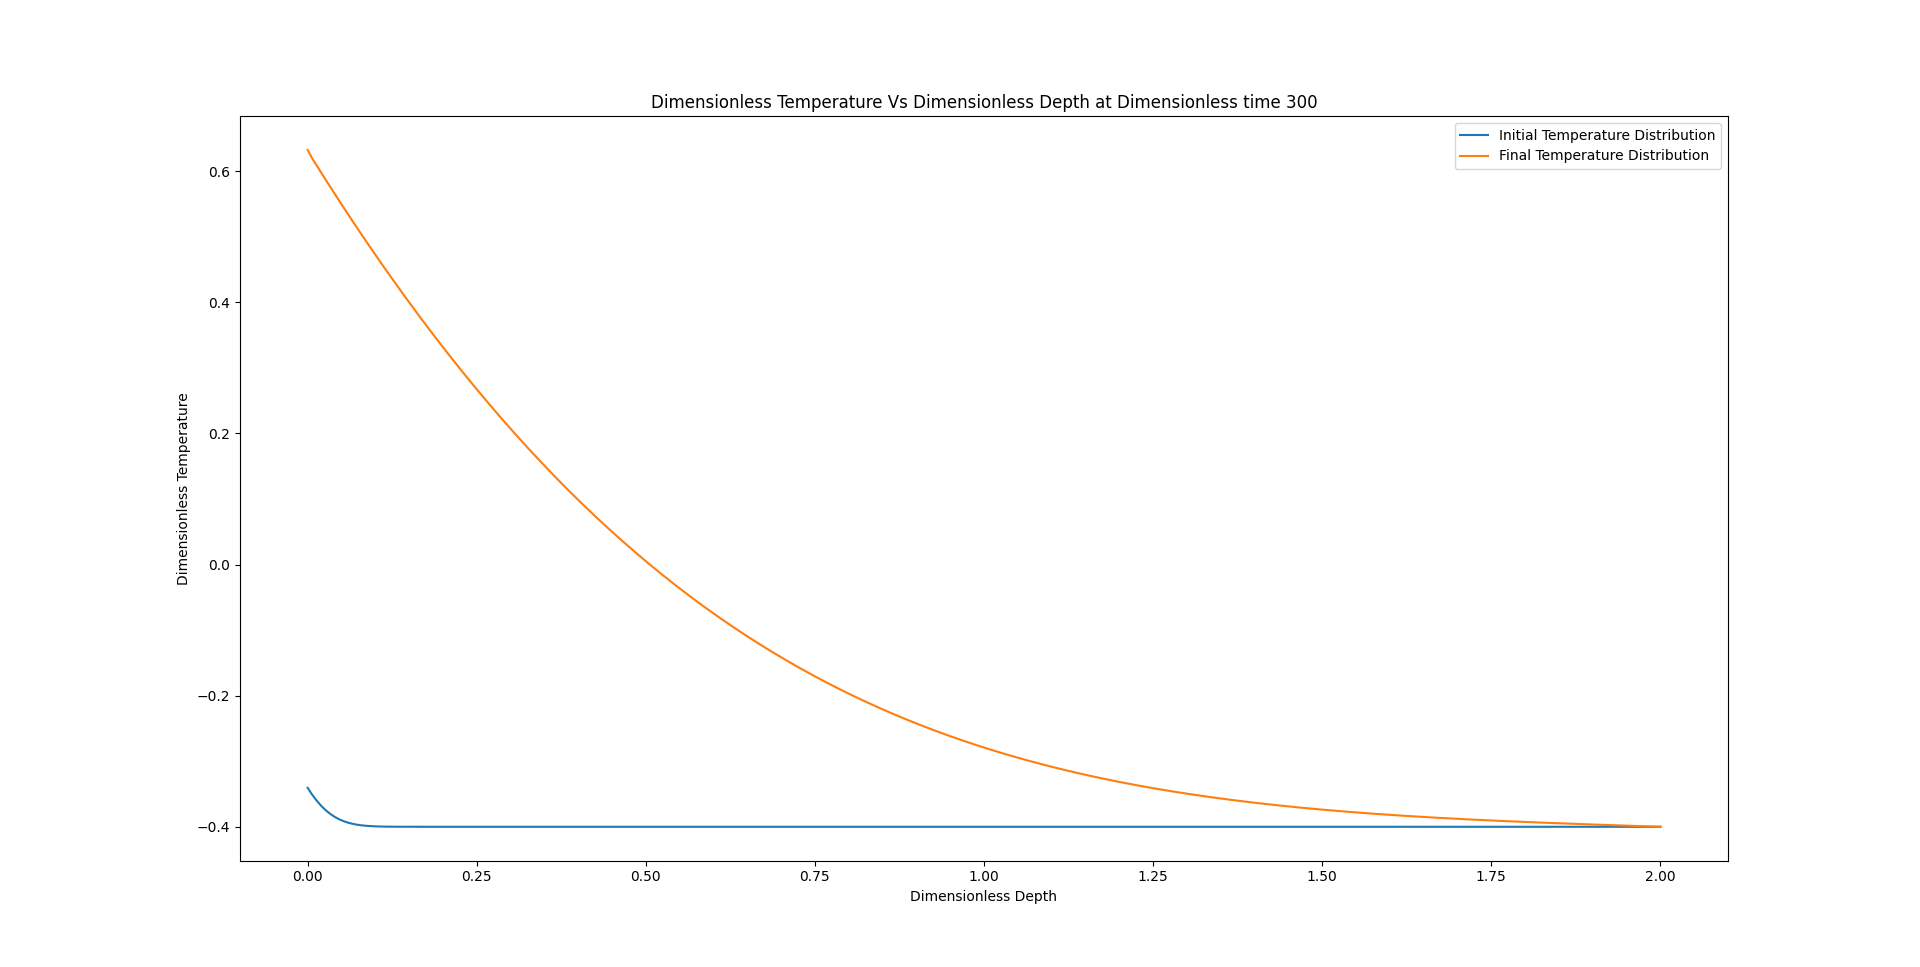
\includegraphics[width=15cm]{img/Temperature_Distribution_in_crystalline_material_Without Latent_Heat_Effects.png}
  \caption{Temperature Distribution in Al (n = 301 nodes, without considering latent heat effects)}
  \label{fig:Temperature Distribution in AL}


  \centering
  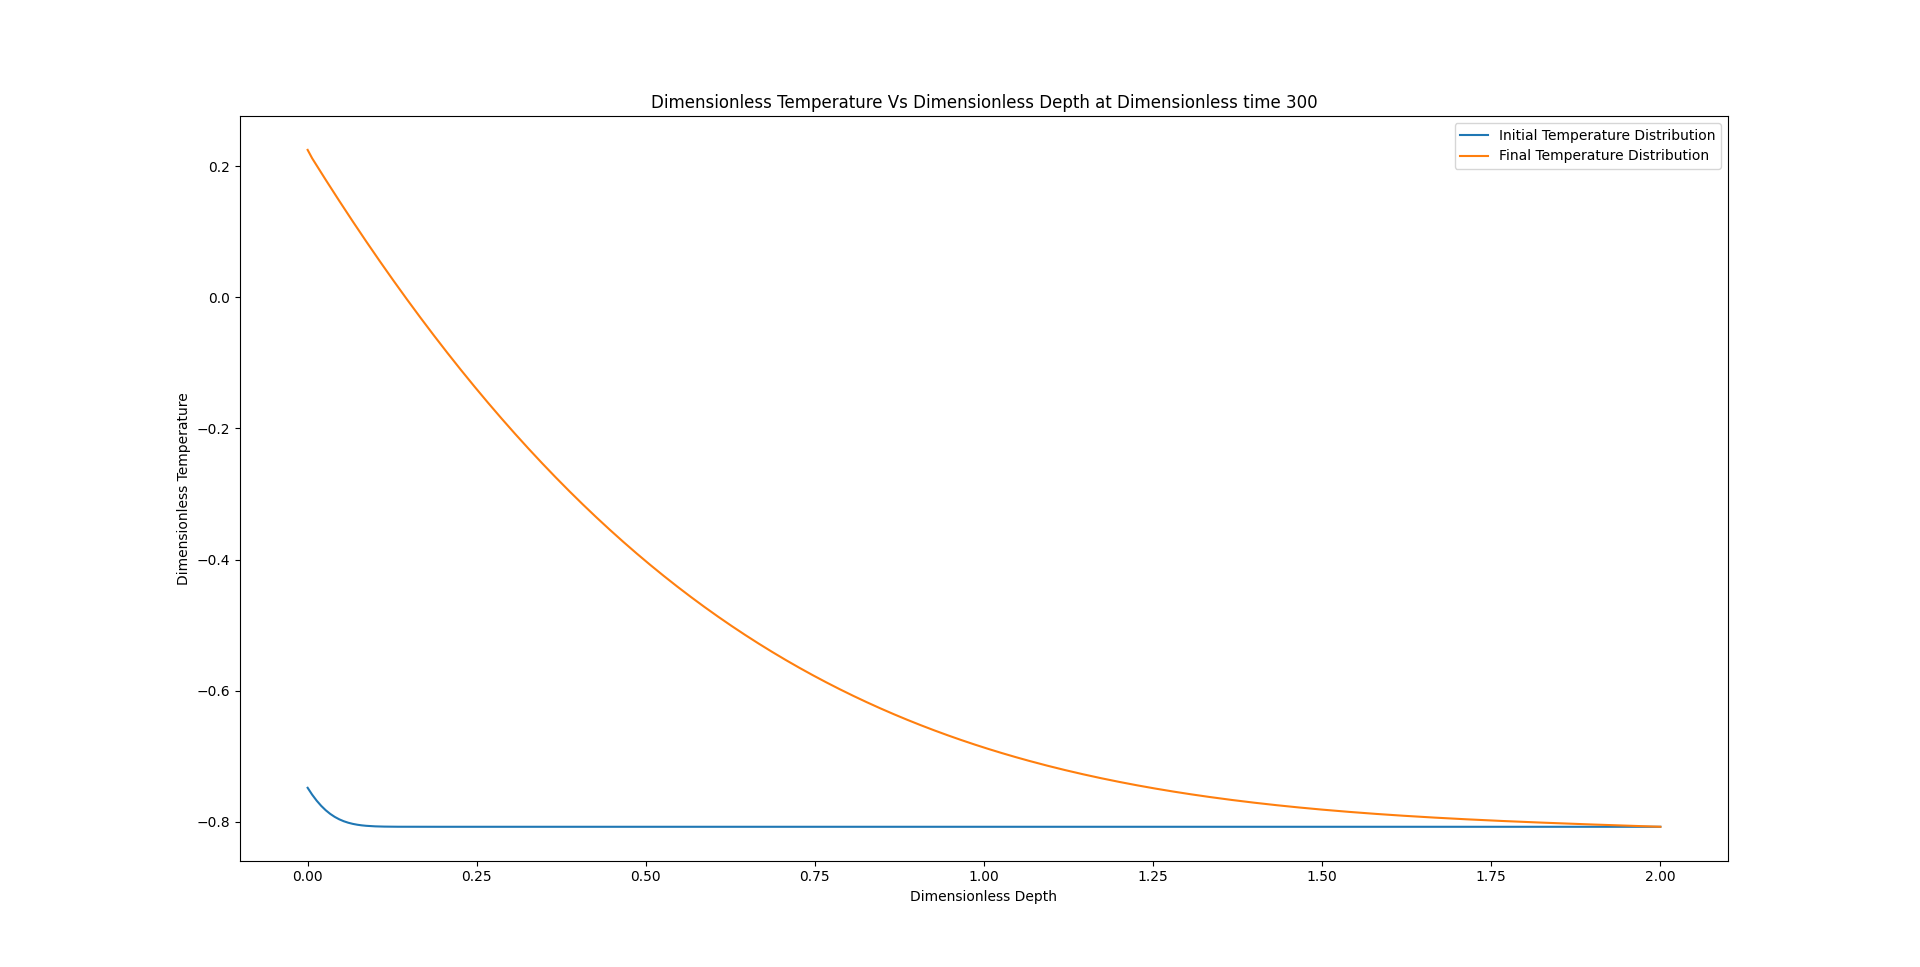
\includegraphics[width=15cm]{img/Temperature_Distribution_Amorphous.png}
  \caption{Temperature Distribution in SS304L (n = 301 nodes, without considering latent heat effects)}
  \label{fig:Temperature Distribution in SS304}
  
\end{figure}


\newpage
\section{Stefan Problem\label{sec:implaspects}}

Similar to the enthalpy problem approach, we present the results form the Stefan problem approach. For the analytical solution of the position of interface over time we employ the Euler Forward time integration scheme on the equation \ref{eq:analytical solution to the position}  and equation \ref{eq:derivativemelt_anal}. This analytical solution does not account for the latent heat. Also, due to the boundary condition \ref{eq:Stefan_specialBc}, we cannot set our latent heat equal to zero. Doing so will not allow our material to melt. Also, it is important to note that this scheme is not applicable to the amorphous material as it does not have sharp melting point. We have assumed $I = 1.5 \times 10^{10} \frac{W}{m^2}$ laser input intensity and 2 nodes in the liquid domain and 51 nodes in the solid domain for the following simulation results. The decision to employ only 2 nodes in the liquid domain was based on the initial conditions, where the liquid domain is minimal, if not negligible. The $\Delta t$ was assumed to be  0.00001.  
\begin{figure}[h]
  \centering
  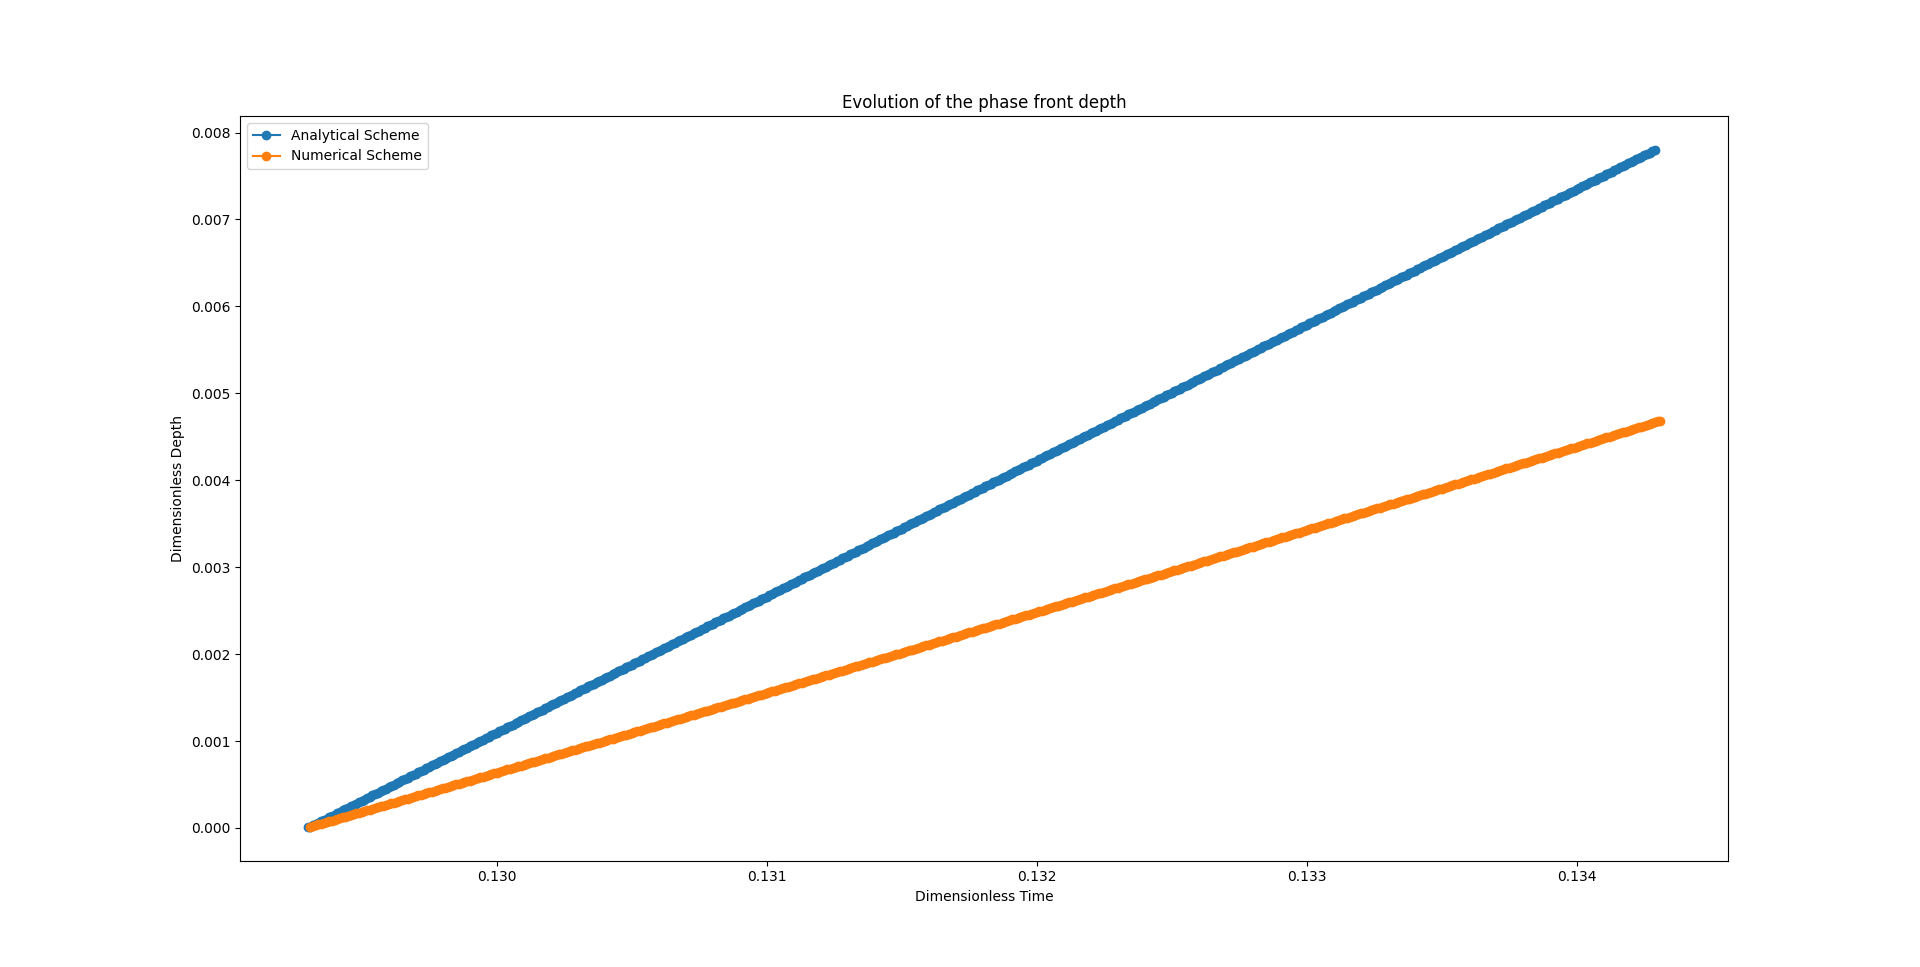
\includegraphics[width=15cm]{img/StefanMelting.png}
  \caption{Position of the phase front from numerical scheme (considering the latent heat) and analytical scheme (neglecting the latent heat effects)}
  \label{fig:Stefan melt phase front}
  \centering
  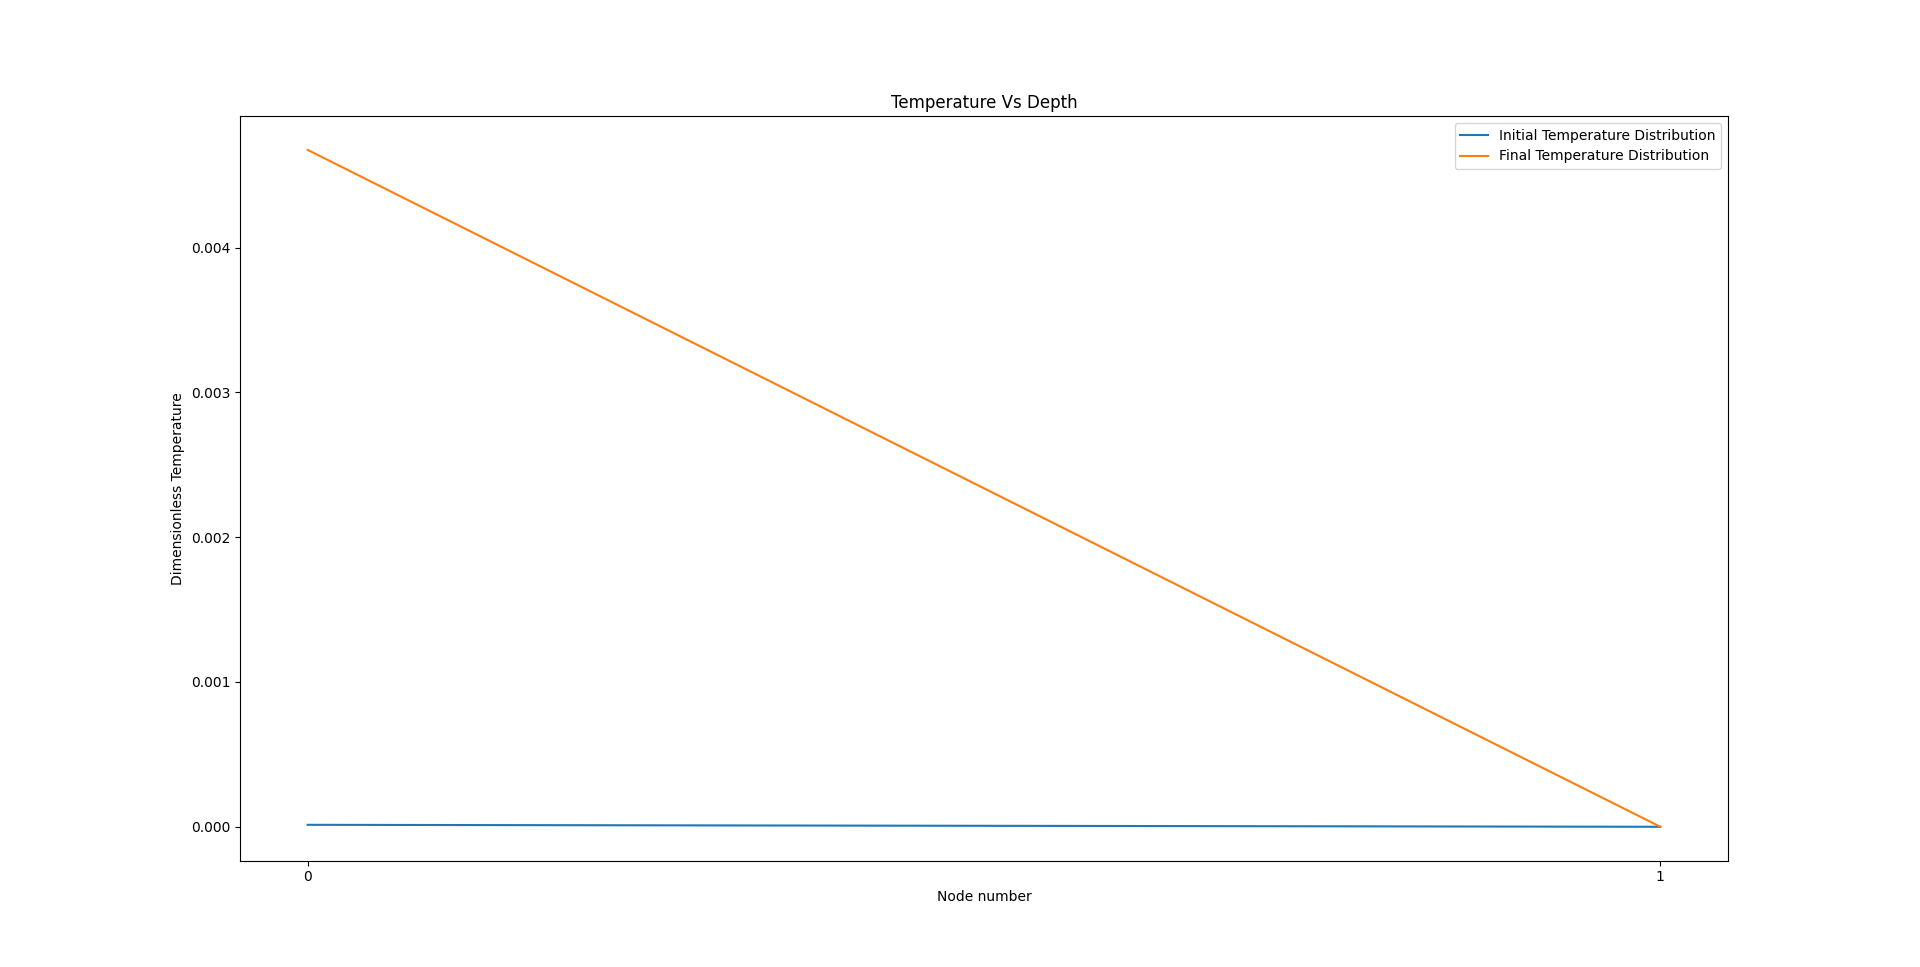
\includegraphics[width=15cm]{img/Stefan_Temp1.png}
  \caption{Temperature distribution in the liquid domain}
  \label{fig:Stefan liq temp}
  \end{figure}
  \begin{figure}[h]
  \centering
  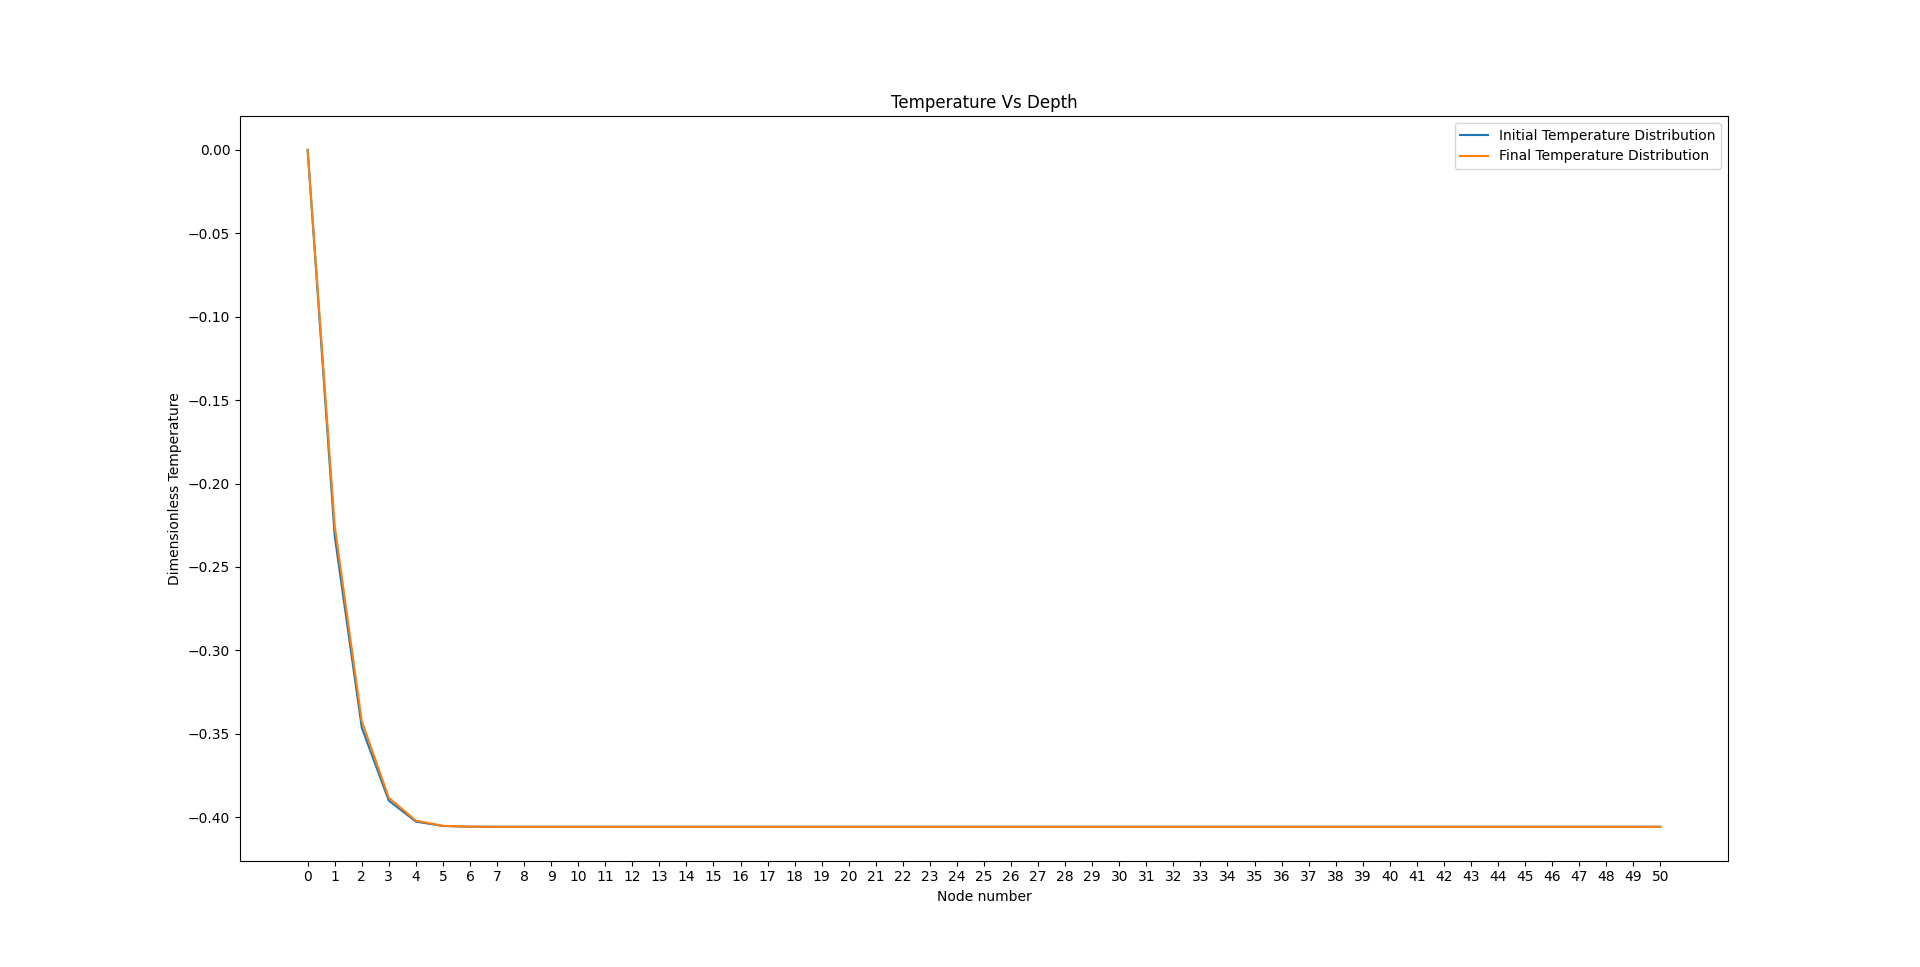
\includegraphics[width=14cm]{img/Stefan_Temperature2.png}
  \caption{Temperature distribution in the solid domain}
  \label{fig:Stefan melt front}
\end{figure}

\subsection{Enthalpy Problem 2D results}
Again we assumed a unit square. We supplied the top left corner node with the laser input. The bottom and the right edge were kept at constant ambient temperature. The results figure \ref{fig:settings for the 2D enthalpy problem} shows the simulation setup. 

\begin{figure}[h]
  \centering
  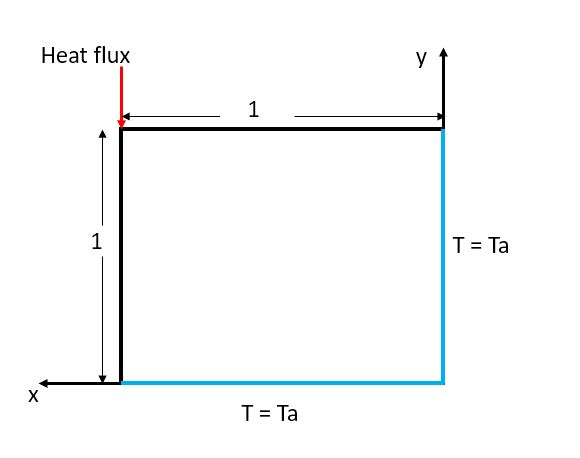
\includegraphics[width=7cm]{img/2Dsetup.png}
  \caption{Settings for the 2D Enthalpy problem}
  \label{fig:settings for the 2D enthalpy problem}
\end{figure}

\begin{figure}[h]
  \centering
  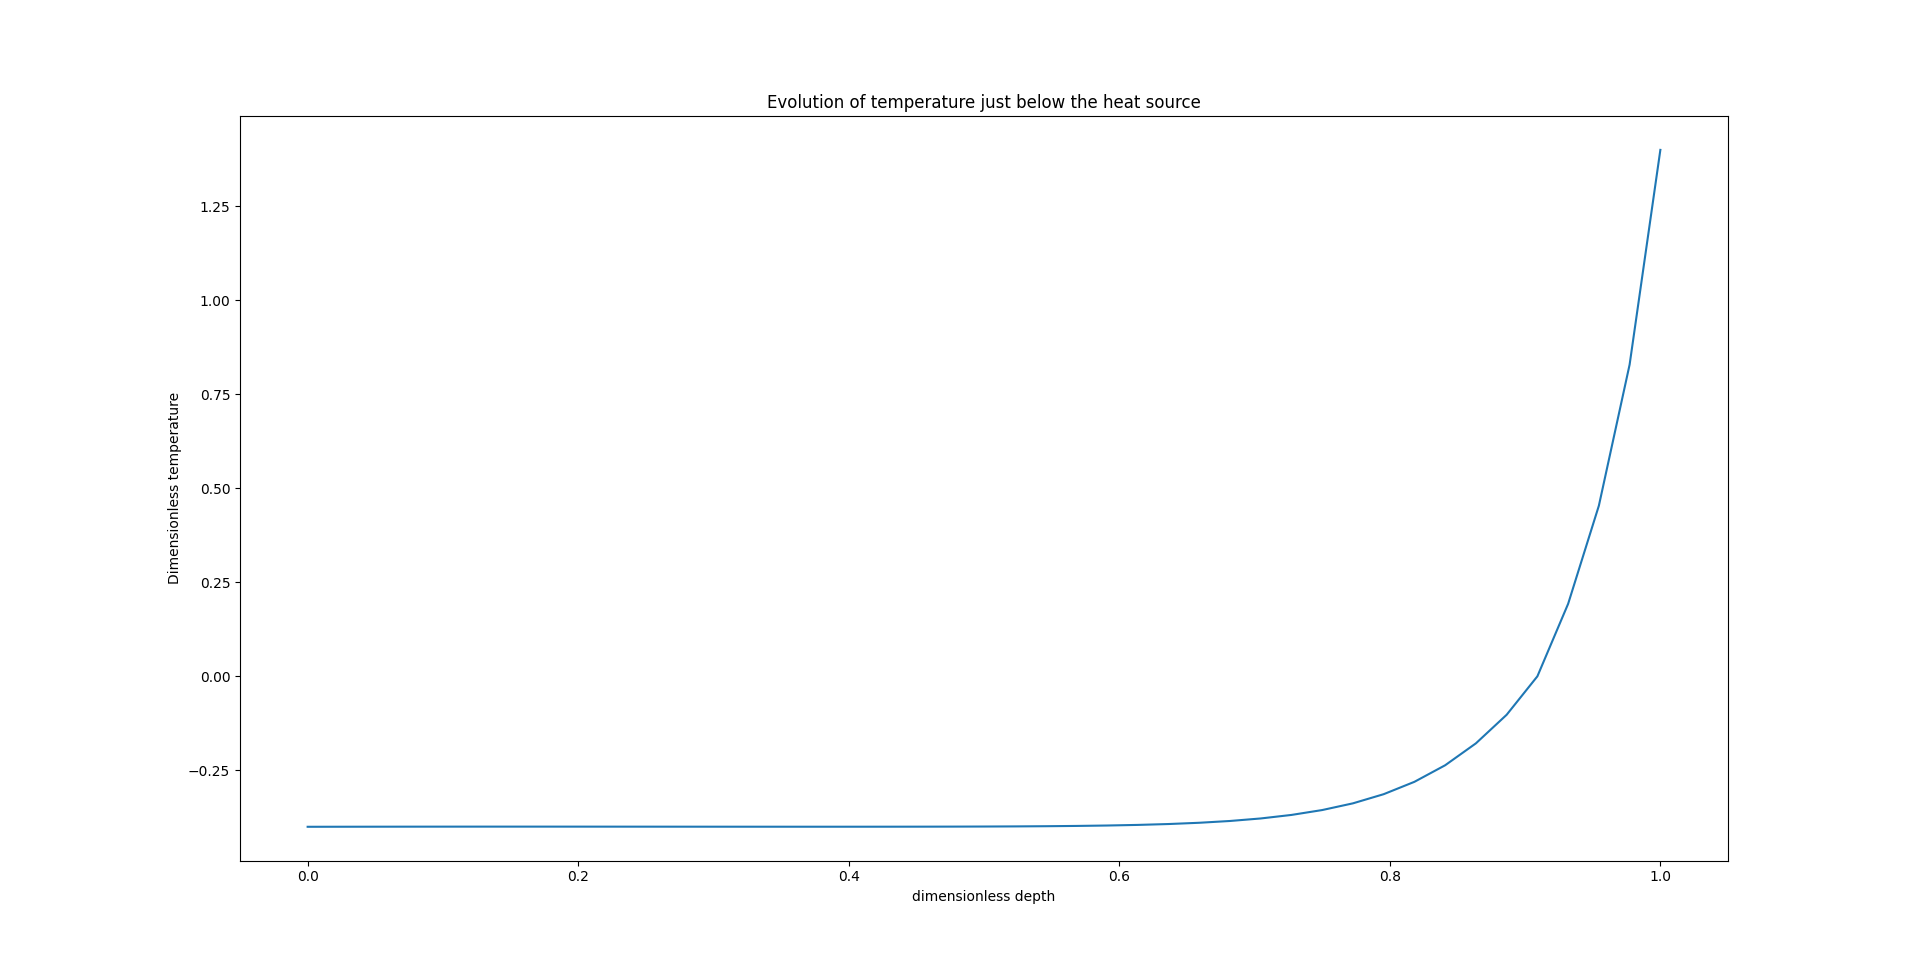
\includegraphics[width=14cm]{img/2D_Enthalpy_Temperature.png}
  \caption{Temperature evolution from the node just below the heat source}
  \label{fig:Temp just below node}
\end{figure}
The figure \ref{fig:Temp just below node} shows the evolution of the temperature over the entire simulation time.  
\begin{figure}[h]
  \centering
  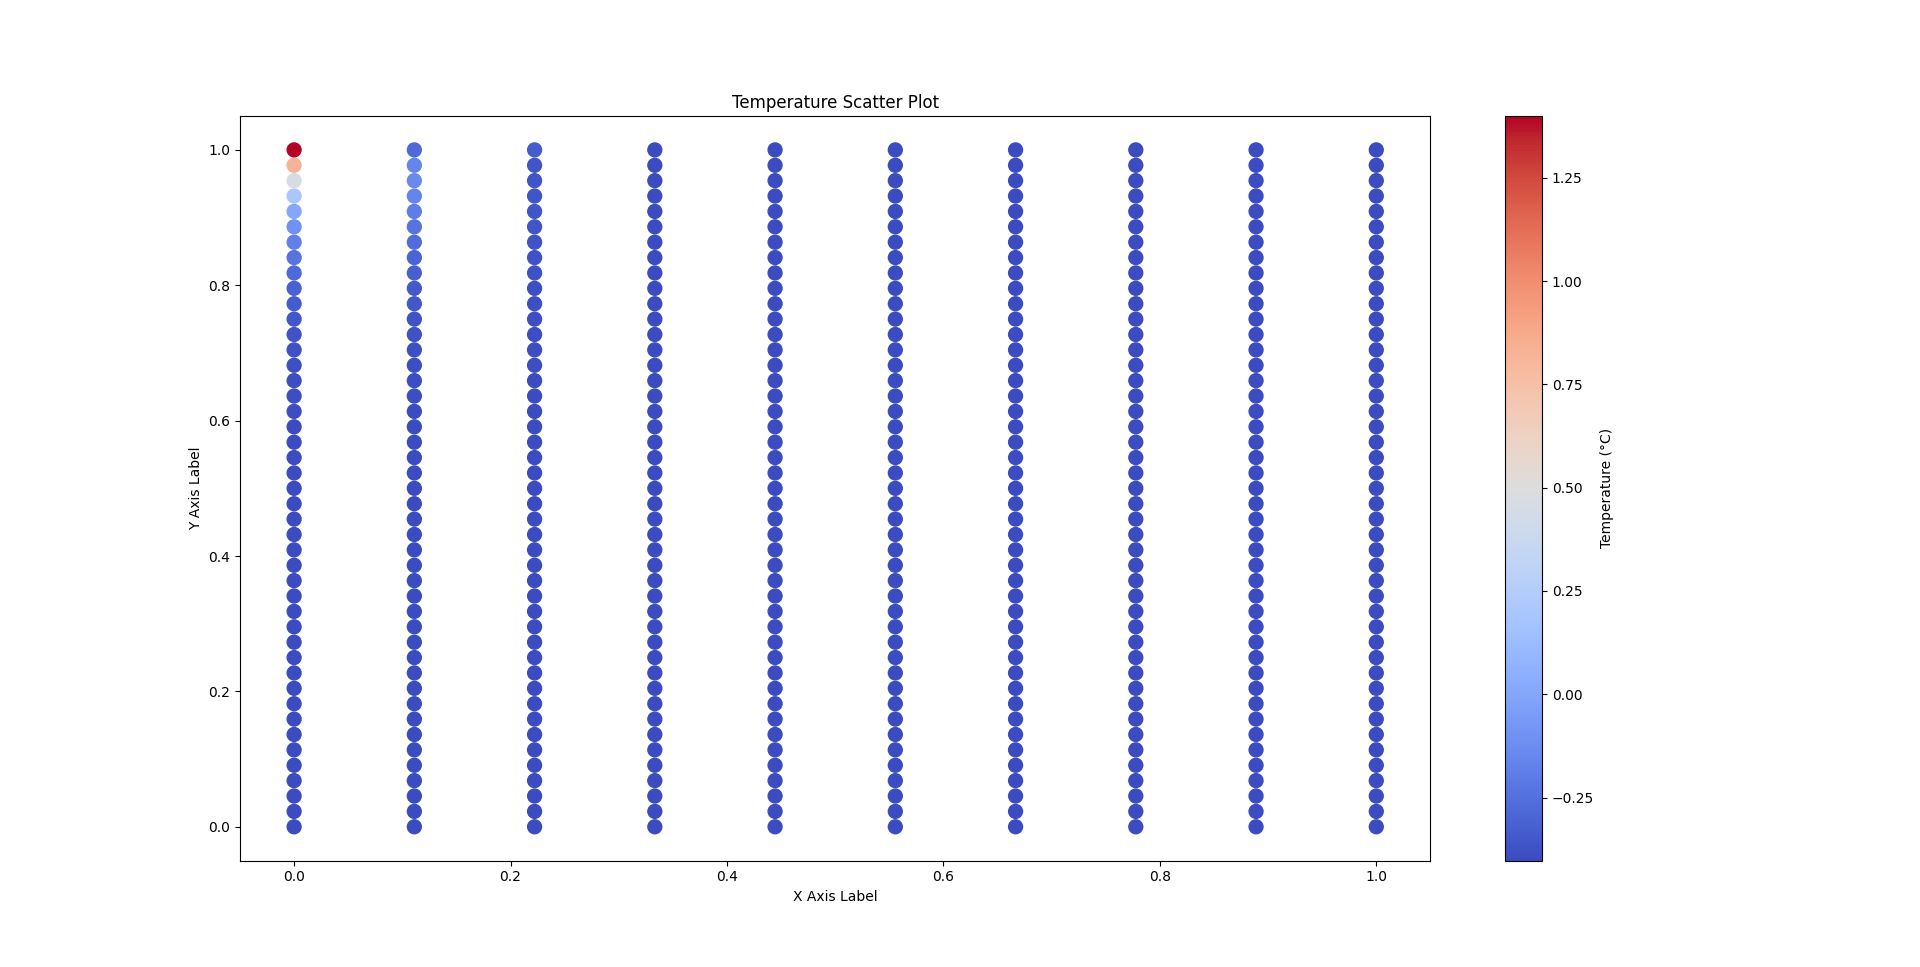
\includegraphics[width=14cm]{img/Temp_2D_Dist_Enthalpy.png}
  \caption{Temperature distribution in the matrix at end time}
  \label{fig:matrix temp end time}
\end{figure}
The figure \ref{fig:matrix temp end time} shows the temperature distribution over the entire domain at the end of simulation time. We can see that first few nodes are in the liquid regime. It is also important to note that the scheme shows convergence issues, when the temperature at node 0 goes beyond unity as it physically means that the material is evaporated. 
\newpage
\chapter{User Manual}{\label{cha:Manual}}

\section{List of files and folders}
\subsection{Enthalpy\_Approach\_1D}
\begin{enumerate}
    \item Amorphous\textunderscore inputs.py
    \item Crystalline\textunderscore inputs.py
    \item Elemental\textunderscore Subroutine.py
    \item FEA\textunderscore solve.py
    \item Initial\textunderscore Temperature\textunderscore Dist.py
    \item Material\textunderscore Subroutine.py
    \item Mesh.py
    \item postProcessor.py
    \item Processed\textunderscore inputs.py
    \item variableUpdater.py
\end{enumerate}
\subsection{Enthalpy\_Approach\_2D}
\begin{enumerate}
    \item Amorphous\textunderscore inputs.py
    \item Crystalline\textunderscore inputs.py
    \item Elemental\textunderscore Subroutine.py
    \item FEA\textunderscore solve.py
    \item Gridify.py
    \item Initial\textunderscore Temperature\textunderscore Dist.py
    \item Material\textunderscore Subroutine.py
    \item Processed\textunderscore inputs.py
    \item variableUpdater.py
\end{enumerate}
\subsection{Heat\textunderscore Transfer\textunderscore Verification}
Along with the above mentioned files the Heat\textunderscore Transfer\textunderscore Verification has one more additional file Heat\textunderscore Transfer\textunderscore Verification.py. The file Initial\textunderscore Temperature\textunderscore Dist.py is changed in this folder. Remaining all the files are same. 
\subsection{Testing}
\begin{enumerate}
    \item Amorphous\textunderscore inputs.py
    \item Crystalline\textunderscore inputs.py
    \item Gridify.py
    \item Mesh.py
    \item Mesh\textunderscore Test.py
    \item Processed\textunderscore inputs.py
    \item Processed\textunderscore inputsA.py
    \item slope\textunderscore matrix.py
    \item Slope\textunderscore MatrixA.py
    \item Test\textunderscore Amorphous.py
    \item Test\textunderscore Crystalline.py
    \item Test\textunderscore Mesh\textunderscore 2D.py
\end{enumerate}
The Gridify.py is the 2D mesh file, Slope\textunderscore MatrixA.py and slope\textunderscore matrix.py are part of Material\textunderscore Subroutine.py. All the other files such as Processed\textunderscore inputs.py and Processed\textunderscore inputsA.py are same just the material selected is different.  
\subsection{Stefan\_ Approach}
\begin{enumerate}
    \item Crystalline\textunderscore inputs.py
    \item Elemental\textunderscore Subroutine.py
    \item FEA\textunderscore solve.py
    \item Initial\textunderscore Conditions.py
    \item postProcessor.py
    \item Processed\textunderscore inputs.py
    \item variableUpdater.py
\end{enumerate}
\section{Libraries used}
The libraries we used in programming the simulation is shown in table \ref{tab:softwares used}. \\
\begin{table}[h]
    \centering
    \begin{tabular}{|c|c|} \hline 
         \textbf{Library / Software}& \textbf{Version}\\ \hline 
 Python &3.11.2\\ \hline 
         Numpy& 1.24.1\\ \hline 
         math& 3.5\\ \hline 
         matplotlib& 3.6.3\\ \hline
 Time&3.11.2 (inbuilt)\\\hline
    \end{tabular}
    \caption{Libraries used and their versions}
    \label{tab:softwares used}
\end{table}
\noindent The installation of the libraries mentioned in table \ref{tab:softwares used} can be done as follows:-\\
Installing the numpy.\\
\indent \indent \$ pip install numpy\\
Installing the math.\\
\indent \indent \$ pip install math\\
Installing the numpy.\\
\indent \indent \$ pip install matplotlib\\
\section{Running the program}
\begin{enumerate}
    \item To begin, please navigate to the folder that contains the files related to the simulation you desire to run.
    \item   The files 'Amorphous\textunderscore inputs.py' and 'Crystalline\textunderscore inputs.py' contains the inputs which can be edited for user defined inputs.
    \item Next, select the type of material in the 'Processed\textunderscore inputs.py' by setting the mat\textunderscore type = 1 for the crystalline material and 2 for the amorphous material for the enthalpy problem approach. Note for Stefan problem approach this variable is always = 1.
    \item    Afterward the simulation can be run using the command line with the command python .\textbackslash FEA\textunderscore solve.py for standard Windows operating system.
    \item Finally, the results will be displayed as graphs and on the command line as well.
\end{enumerate}
\newpage
\chapter{Computation time study}{\label{cha:Computational Study time}}
The 'time' module is built into the Python interpreter, and we have utilized this module in our program to measure the time required for the execution of each module. The modules and their respective execution times are presented in Table \ref{tab:computational time study}.\\
\begin{table}[h]
    \centering
    \begin{tabular}{|c|c|} \hline  
         \textbf{Library}& \textbf{Time} (in s)\\ \hline  
         Mesh& 0\\ \hline  
 Gridify&0.01\\ \hline 
         Initial\textunderscore Temperature\textunderscore Dist& 0\\ \hline  
         variableUpdater& 0\\ \hline  
         Elemental\textunderscore Subroutine& 0.491\\ \hline  
         FEA\textunderscore solve& 16.3031\\ \hline  
         postProcessor& 9.6406\\ \hline 
    \end{tabular}
    \caption{Computation time study}
    \label{tab:computational time study}
\end{table}
It can be observed that the solver requires the most time to execute. In the previous versions of the program, where the assembly was done using the assignment matrix, the time required was quite large. Introduction of mesh list removed the need of assignment matrix. Hence, an improvement in the computational time was observed. Further, the computational time can be reduced by utilizing the 'scipy' package in python which includes a sparse matrix solver. This solver is considerably more efficient than computing the inverse of the stiffness matrix, which is computationally expensive. Additionally, the assembly is now done in a separate function, which allows parallelization of the execution.
    \chapter{Conclusion\label{cha:chapter7}}
In conclusion, we have successfully developed a program to track the location of the solid liquid phase front using two approaches: the Enthalpy problem approach and the Stefan problem approach. The former method is referred to as a fixed domain method, while the latter is referred to as a front tracking method.\\
In the fixed domain method, the temperature-enthalpy relation is used to track the phase front.On the other hand, the front tracking method employs the Arbitrary  Euler-Lagrange Approach to track the position of the phase front. The fixed grid method is applicable to both amorphous and crystalline materials, while the variable space grid can only be employed for crystalline materials.\\
In the Enthalpy problem approach, for both amorphous and crystalline materials, we validated two cases for the heat transfer verification. The first case with both the ends at a fixed temperature, usually referred to as type I boundary condition, and the second case includes one end at a fixed temperature and other end insulated, commonly referred to as type II boundary condition. In both the cases, we observed a good agreement with the analytical solution. We also conducted a mesh convergence test and found an exponential decay in errors after 300 nodes.\\
For the type II boundary condition, we analyzed the effect of adding a term to the analytical solution. The location of the phase front was tracked successfully using this method and was compared with the analytical scheme.  A staircase-like behaviour in the solution of the phase front location for lower number of nodes from the Enthalpy problem approach was observed. Additionally, we encountered a convergence issue during the phase transition in the 2D fixed grid method due to the the temperature at the first node crossing the vaporisation temperature, making the problem unphysical. \\
We also compared the location of interface obtained from the variable space grid method. The solution exhibited a good trend with the analytical one, but exact overlap is not achieved due to the latent heat effects. Further, in 2D settings, we saw for the fixed grid method we employed the new numerical approach as suggested by Zhao-chun Wu \cite{Wu+2005+281+288}. However, his method has issues with the velocity update.\\
The entire program was built using Object-Oriented Programming, as methods can be passed to a function or another method along with the attributes by just passing an instance of a class, allowing simplicity in programming. \\

\section{Problems Encountered and Experiences\label{sec:problems}}

Earlier, for one dimensional Enthalpy problem approach, only type II boundary condition for the verification of the heat transfer was planned. The heat transfer results from the scheme showed an acceptable agreement with the analytical one with some stability issues.\\
Later, I decided to independently verify the results of heat transfer for a type I boundary condition to assess the stability condition. During this second verification, the results exhibited a bias toward the end where heat flux was applied. Upon performing manual calculations to investigate this bias, it was discovered that the input laser had not been correctly turned off. The scheme was so designed that laser power in the inputs script would be overridden by the material model. This was due to the Object-Oriented programming where the instance of the material model was not lost even after the function execution was completed. This led to inaccuracies throughout the scheme. 
\textbf{Lessons Learnt:} While Object-Oriented Programming can be advantageous for passing attributes and methods, it's important to be aware that, unlike functions where the scope of a variable is limited to within the function, and the variable is lost once the function is completed, the attributes of a class are not lost and retain the data from the previous calculation unless explicitly reset or reinitialized. This also highlights the importance of the testing and verification of the code for various cases.

\section{Acknowledgement\label{sec:Acknowledgement}}

I extend my sincere gratitude to Dr. Ing. Stefan Prüger for his invaluable assistance at every stage of this project, particularly in the verification of the type I and II boundary conditions. His guidance and insights were of great help in addressing challenges, understanding the physics and enhancing the overall quality of the work.\\

I would also like to acknowledge the contributions of authors of the paper 'Modelling laser induced melting'  Verhoeven J.C.J, Jansen, J. K. M., Mattheij, R. M. M., and Smith, W. R. whose mathematical formulation served as the foundation for implementing the Finite Element Method (FEM) scheme in our project.\\

Lastly, I am thankful to TU Berlin for providing the LaTeX template on Overleaf, enabling us to produce this work seamlessly and efficiently.
\newpage
\section{Milestones - status\label{sec:Milestone}}


\begin{table}[h]
    \centering
    \begin{tabular}{|c|c|} \hline 
         Milestone& Status\\ \hline 
         Programming of the 1D Enthalpy problem& Yes\\ \hline 
         Heat Transfer Verification with type I boundary condition& Yes\\ \hline 
         Heat Transfer Verification with type II boundary condition& Yes\\ \hline 
         Verification of the position of the phase front& Yes\\ \hline 
         Programming of the 1D Stefan problem& Yes\\ \hline 
         Verification of the position of the phase front & Yes\\ \hline 
         Programming of the 2D Enthalpy problem& Yes\\ \hline 
 Programming of the 2D Stefan problem &Yes\\ \hline
    \end{tabular}
    \caption{Milestone status of the project}
    \label{tab:Milestone status}
\end{table}


% ---------------------------------------------------------------
\backmatter % no page numbering from here
    \addchap{Nomenclature}
Tensors and vectors are represented in bold with an underline (\textbf{\underline{A}})
\subsection{Constants}
\begin{tabbing}
spacespacespace \= space \kill
$\rho$	 \> 	Density ($\frac{kg}{m^3}$)	 \\
c	\>	Specific Heat Capacity ($\frac{J}{kg K}$)\\
k	 \> 	Thermal Conductivity $\frac{W}{m K}$ \\
$I_ref$	\>	Reference laser energy $\frac{W}{m^2}$ \\
$\theta_v$	\>	Vapourisation Temperature K \\
$\theta_m$	\>	Melting Temperature K \\
$ T_v $	\>	Non dimensionalised vapourisation temperature \\
$ T_m$	\>	Non dimensionalised melting temperature \\
\end{tabbing}
\subsection{Variables}
\begin{tabbing}
spacespacespace \= space \kill
$\tau$	 \> 	Time (s)	 \\
$\theta$	\>	Temperature (K) \\
$\chi$	\>	Depth in z direction (m) \\
r	\>	Radius (m) \\
I	\>	Laser input energy $\frac{W}{m^2}$ \\
$w_0$	\>	Waist m\\
z	\>	Non dimensionalised depth \\
$\bar{r}$	\>	Non dimensionalised radius \\
t	\>	Non dimensionalised time\\
T	\>	Non dimensionalised temperature \\
$L_f$ \> Latent heat of fusion \\
$s$ \> Position of the solid liquid interface\\
\end{tabbing}
\subsection{Subscripts}
\begin{tabbing}
spacespacespace \= space \kill
0	 \> 	initial or starting value\\
s	\>	solid domain\\
l	\>	liquid domain \\
sol	\>	Solidus \\
liq	\>	Liquids  \\
$w_0$	\>	Waist m\\
z	\>	Non dimensionalised depth \\
$ \bar{r} $	\>	Non dimensionalised radius \\
t	\>	Non dimensionalised time\\
T	\>	Non dimensionalised temperature \\
\end{tabbing}
\endinput

		
		% if you want to provide a glossary with explanations of important terms put it in here

    \bibliographystyle{plain}
    \bibliography{./bib/manual}
    
    \newpage
\section{Git Log}
\lstset{
  basicstyle=\footnotesize\ttfamily,
  breaklines=true,
  frame=single,
}

\lstinputlisting{gitlog.txt}

\end{document}
